\section{Dark Matter and Weakly Interacting Particles}
\subsection{Introduction}
\subsection{Cosmological Preliminaries}
\subsection{Observational Evidence for Dark Matter Existance}
\subsection{Supersymmetry}
\subsection{Simplified Models}
\subsection{Effective Field Theories at the LHC}
\subsection{Introduction}

The existence of dark matter (DM) in the universe, originally proposed~\cite{Zwicky:1937zza} to
reconcile observations of the Coma galaxy cluster with
the prediction from the virial theorem, is 
commonly accepted as the explanation of many experimental
phenomena in astrophysics and cosmology, such as galaxy rotation
curves~\cite{vandeHulst,Rubin:1980zd}, large structure
formation~\cite{White:1987yr,Carlberg:1989yr,Springel:2005nw}, and the
observed
spectrum~\cite{Smoot:1992td,deBernardis:2000gy,Spergel:2006hy,Ade:2013zuv}
of the cosmic microwave background~\cite{Bardeen:1985tr}. A global fit to
cosmological data in the so-called $\Lambda$CDM model (also known as
the standard model of cosmology)~\cite{Cen:2000xv} suggests that
approximately $85\%$ of the mass of the universe is made of
DM~\cite{Ade:2013zuv}. To accommodate these observations and the
dynamics of colliding galaxy clusters, it has been
hypothesized~\cite{Clowe:2006eq} that DM is made mostly of weakly
interacting massive particles
(WIMPs), sufficiently massive to be in nonrelativistic motion
following their decoupling from the hot particle plasma in the early
stages of the expansion of the universe.

While the standard model (SM) of particle physics does not include a
viable DM candidate, several models of physics beyond the SM, e.g.
supersymmetry (SUSY)~\cite{Ramond,Golfand,Volkov,Wess,Fayet} with R-parity
conservation, can accommodate the existence of WIMPs. In these models,
pairs of DM particles can be produced in proton-proton (pp) collisions at
the CERN LHC. Dark matter particles would not leave a detectable signal in
a particle detector. When produced in association with high-energy
quarks or gluons, they could provide event topologies with
jets and a transverse momentum (\pt) imbalance ($\vec{p}_{\rm T}^{\rm miss}$). 
The magnitude of $\vec{p}_{\rm T}^{\rm miss}$ is referred to as missing transverse energy ($E_{\rm T}^{\rm{miss}}$).
%The online trigger system at hadron colliders records such events for
%use in analyses. 
%Similar searches have already been
%performed by the LHC collaborations on events
%with one large-\pt jet and an imbalance in $\vec{p}_{\rm T}^{\rm
% miss}$~\cite{Aad:2011xw,Chatrchyan:2012me}. 
The ATLAS and CMS collaborations have reported
~\cite{Aad:2011xw,Chatrchyan:2012me} searches for events with one
high-\pt jet and large $\vec{p}_{\rm T}^{\rm miss}$, which are sensitive to such topologies.
In this paper, we refer to these studies as monojet searches. Complementary studies of events with
high-\pt photons~\cite{Khachatryan:2014rwa,Aad:2014tda}; \PW,
\cPZ,~or
higgs~bosons~\cite{Aad:2013oja,Aad:2014vka,Aad:2015dva,Aad:2015yga};
b-jets~\cite{Aad:2014vea} and top quarks~\cite{Aad:2014vea,CMS:b2g12-022,CMS:semilepTop}; and leptons~\cite{ATLAS:2014wra,Khachatryan:2014tva}
have also been performed.

This paper describes a search for DM in events with at least two jets of comparable transverse momentum
and sizable $\vec{p}_{\rm T}^{\rm miss}$. The search is based 
on the razor variables $\mathrm{M}_{\rm R}$ and $\mathrm{R}^2$~\cite{rogan,razor2010}.  Given a
dijet event, these variables are computed from the two jet momenta
$\vec{p}^{{{\hspace{0.04cm}\rm j}_{1}}$ and
$\vec{p}^{{{\hspace{0.04cm}\rm j}_{2}}$, according to the following
definition:
\begin{eqnarray}
 \label{eq:MRstar}
 \mathrm{M_{\rm R}}  & \equiv & 
 \sqrt{
  (|\vec{p}^{{\hspace{0.04cm}\rm j}_{1}}|+|\vec{p}^{{\hspace{0.04cm}\rm j}_{2}}|)^2 -
  (p^{{\rm j}_1}_{\rm z}+p^{{\rm j}_2}_{\rm z})^2}\;,\nonumber
\\
 \mathrm{R}  & \equiv &  \frac{\mathrm{M^R_T}}{\mathrm{M_{\rm R}}}\; ,
\label{eq:razor}
\end{eqnarray}
with
\begin{eqnarray}
 \label{eq:MTR}
 \mathrm{M_T^R}  & \equiv &  \sqrt{ \frac{E_{\rm T}^{\rm{miss}}(\pt^{{\rm j}_1}+\pt^{{\rm j}_2}) -
   \vec{p}_{\rm T}^{\rm{miss}} {\mathbf \cdot}
   (\vec{p}_{\rm{T}}^{\,{\rm j}_1}+\vec{p}_{\rm{T}}^{\,{\rm j}_2})}{2}} \; .
\end{eqnarray}

In the context of SUSY, $\mathrm{M_{\rm R}}$ provides an estimate of the
underlying mass scale of the event. The quantity $\mathrm{M_T^R}$ is a transverse
observable that includes information about the
topology of the event. The variable $\mathrm{R}^2$ is designed to reduce QCD
multijet background; it is correlated with the angle
between the two jets, where co-linear jets have large $\mathrm{R}^2$ while back-to-back jets have small $\mathrm{R}^2$.
These variables have been used to study the production of invisible
particles in cascade decays of heavier partners, such as squarks and
gluinos in models of SUSY with $\math{R}$-parity
conservation~\cite{Chatrchyan:2014goa,Razor8TeV}. The sensitivity of
these variables to direct DM production was suggested in
Ref.~\cite{Fox:2012ee}, where it was pointed out that the dijet event
topology provides good discrimination against background processes
with a looser event selection than that applied in the monojet searches. %This fact compensates
%The signal to background discrimination and the inclusive selection for the reduction in signal cross section because of the requirement
%of additional jets in the final state.
The resulting sensitivity is comparable to that of monojet searches~\cite{Fox:2012ee,Papucci:2014iwa}. This
strategy also offers the possibility to search for DM particles that
couple preferentially to b quarks~\cite{Agrawal:2014una}, as proposed
to accommodate the observed excess of photons with energies between
1 and 4 GeV in the gamma ray spectrum of the galactic centre data collected by the Fermi-LAT gamma-ray space
telescope~\cite{Hooper:2010mq}. The results are interpreted using an
effective field theory approach and the Feynman diagrams for DM pair production are shown in Fig.~\ref{fig:DMdiamgrams}.

\begin{figure}[h!]
 \centering
 \begin{tabular}{cc}
    \hspace{-1cm}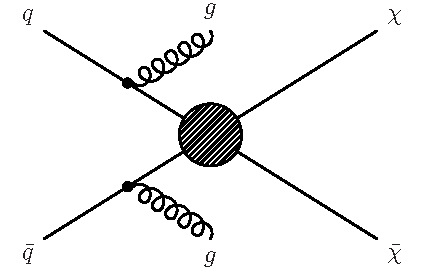
\includegraphics[width=0.35\textwidth]{DarkMatter8TeV/Diagrams/RazorDMdiagram.pdf}  & 
   \hspace{1cm}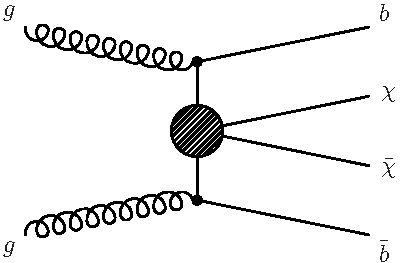
\includegraphics[width=0.3\textwidth]{DarkMatter8TeV/Diagrams/RazorDM_bTagV2.pdf}
  \end{tabular}
 \caption{Feynman diagrams for the pair production of DM particles
   corresponding to an effective field theory using (left) a vector or
   axial-vector operator, and (right) a scalar operator.\label{fig:DMdiamgrams}}
\end{figure}

% This analysis does not consider models of DM production in
%association with Z bosons or $\ttbar$ systems that would populate both
%signal and control regions. These kinds of models are covered by other
%searches~\cite{Aad:2013oja,Aad:2014vka,Aad:2014vea,CMS:b2g12-022,CMS:2014mxa,CMS:semilepTop}.

Unlike the SUSY razor searches~\cite{Razor8TeV,razor2010}, which focus on events with large
values of $\mathrm{M_{\rm R}}$, this study also considers events with small values
of $\mathrm{M_{\rm R}}$, using $\mathrm{R^2}$ to discriminate
between signal and background, in a kinematic region ($\mathrm{R^2} >
0.5$) excluded by the baseline selection of Refs.~\cite{Razor8TeV,razor2010}.

A data sample corresponding to an integrated luminosity of
$18.8$~\fbinv of pp collisions at a center-of-mass energy of
$\sqrt{s}=8$~TeV  was collected by the CMS experiment % at the CERN LHC
%Proton-proton collisions were collected at $\sqrt{s}=8$~TeV by the CMS
%experiment~\cite{Chatrchyan:2008zzk} at the CERN LHC, corresponding to
%an integrated luminosity of $18.8$~\fbinv
 with a trigger based on a
loose selection on $\mathrm{M_{\rm R}}$ and $\mathrm{R^2}$. This and other
special triggers were operated in 2012 to record events at a rate
higher than the CMS computing system could process during data
taking. The events from these triggers were stored on tape and their
reconstruction was delayed until 2013, to profit from the larger availability of processing resources during the LHC shutdown. 
%These data are referred to as {\it parked} data~\cite{CMS-DP-2012-022}. The parked data
%enabled the exploration of events with small $\mathrm{M_{\rm R}}$
%values, thereby enhancing the sensitivity to direct DM production.
%The result is studied in terms of several DM production models.
These data, referred to as ``parked data''~\cite{CMS-DP-2012-022},
enabled the exploration of events with small $\mathrm{M_{\rm R}}$
values, thereby enhancing the sensitivity to direct DM production.
 
This paper is organized as follows: the CMS detector is briefly described
in Section~\ref{cmsdetector}.  Section~\ref{sec:sample}
describes the data and simulated samples of events used in the
analysis. Sections~\ref{sec:selection} and~\ref{sec:sampleDef} discuss
respectively the event selections and categorization. The
estimation of the background is described in Section~\ref{sec:bkg}.
The systematic uncertainties are discussed in Section~\ref{sec:sys},
while Section~\ref{sec:interpretation} presents the results and the
implications for several models of DM production. A summary and
conclusions are given in Section~\ref{sec:conclusions}.

\section{The CMS detector}\label{cmsdetector}

The central feature of the CMS apparatus is a superconducting solenoid
of 6\unit{m} internal diameter, providing a magnetic field of
3.8\unit{T}. Within the solenoid volume are a silicon
pixel and strip tracker, a lead tungstate crystal electromagnetic
calorimeter (ECAL), and a brass and scintillator hadron calorimeter
(HCAL), each composed of a barrel and two endcap sections. 
%The HCAL, when combined
%with the ECAL, measures jets with a resolution $\Delta E/E \approx
%100\% / \sqrt{E\,[\GeVns]} \oplus 5\%$
When combining information from the entire detector, the jet energy resolution amounts typically to 15\% at 10\GeV, 8\% at 100\GeV, and 4\% at 1\TeV~\cite{Chatrchyan:2013dga}. Muons are
measured in gas-ionization detectors embedded in the steel flux-return
yoke outside the solenoid. Forward calorimeters extend the
pseudorapidity ($\eta$)~\cite{Chatrchyan:2008zzk} coverage provided by the
barrel and endcap detectors. The first level (L1) of the CMS trigger system, composed of custom
hardware processors, uses information from the calorimeters and muon
detectors to select the most interesting events in a fixed time
interval of less than 4\mus. The high-level trigger (HLT) processor
farm further decreases the event rate from around 100\unit{kHz} to
around 400\unit{Hz}, before data storage. A more
detailed description of the CMS detector, together with a definition
of the coordinate system used and the basic kinematic variables, can
be found in Ref.~\cite{Chatrchyan:2008zzk}.

\section{Data set and simulated samples}
\label{sec:sample}
The analysis is performed on events with two jets reconstructed at L1 
in the central part of the detector ($|\eta|< 3.0$). The L1 jet
triggers are based on the sums of %of ECAL and HCAL transverse energy in
%non-overlapping 4$\times$4 trigger towers, and are characterized by
%the transverse energy in 3$\times$3 calorimeter regions, 
%each of which is 0.35$\eta\times$0.35$\phi$ in
%size~\cite{Chatrchyan:2008zzk}. Events passing the L1 selection are
transverse energy in regions $\Delta\eta\times\Delta\phi$
approximately 1.05$\times$1.05 radians in
size~\cite{Chatrchyan:2008zzk} (where $\phi$ is the azimuthal angle, in the plane transverse to the LHC beams.). 
%Events passing the L1 selection are further processed by the HLT.
%, these jets are identified using a 3$\times$3 sliding window algorithm
%running over the region sums
%0.35$\eta\times$0.35$\phi$)~\cite{Chatrchyan:2008zzk}. Subsequently, these events are analize 
%by a dedicated HLT algorithm in the parked dataset.
%The analysis is performed on events collected by a dedicated HLT
%algorithm in the parked dataset. The trigger records events with two
%jets reconstructed at L1. 
At the HLT, energy deposits in ECAL and HCAL are clustered into jets and the
razor variables $\mathrm{R^2}$ and $\mathrm{M_{\rm R}}$ are computed. In the
HLT, jets are defined using the {\scshape FastJet}~\cite{fastjet}
implementation of the anti-k$_{\rm{T}}$~\cite{antikt} algorithm, with
a distance parameter equal to $0.5$. Events with at least two jets with \pt$>64$~\GeV are
considered. Events are selected with $\mathrm{R^2}> 0.09$ and
$\mathrm{R^2} \times \mathrm{M_{\rm R}} > 45$ \GeV. This selection rejects
the majority of the background at low $\mathrm{R^2}$ and low
$\mathrm{M_{\rm R}}$ values while keeping the events in the signal-sensitive
regions of the ($\mathrm{M_{\rm R}}$, $\mathrm{R}^2$) plane. 
%The sametrigger requirement is employed for events with and without
%muons.
The trigger efficiency, measured using a pre-scaled trigger with very loose thresholds, is
shown in Table~\ref{tab:Trigger}.  The requirements described above correspond to the least stringent event selection, given the constraints on the maximum acceptable rate.

\begin{table}[htb]
\begin{center}
  \caption{\label{tab:Trigger}Measured trigger efficiency for different
    $\mathrm{M_{\rm R}}$ regions. The selection $\mathrm{R^2} >$ 0.35 is applied.}
\begin{tabular}{|c|c|c|c|} 
  \hline
  $\mathrm{M_{\rm R}}$ region (GeV) & $200-300$ &  $300-400$ &  $400-3500$ \\
  \hline
  Trigger efficiency (\%) & $91.1\pm ^{1.5}_{1.7}$ & $90.7\pm ^{2.3}_{2.9}$ & $94.4 \pm ^{2.4}_{3.6}$ \\
  \hline
\end{tabular}
\end{center}
\end{table}

Monte Carlo (MC) simulated signal and background samples are generated with the
leading order matrix element generator {\sc MadGraph
  v5.1.3}~\cite{Alwall:2011uj,Alwall:2014hca}. Parton shower and
hadronization effects are included by matching the generated events to
{\sc Pythia} 6.4.26~\cite{Sjostrand:2006za}, using the MLM matching
algorithm~\cite{Hoche:2006ph}. The most recent PYTHIA Z2* tune is derived from the Z1
tune~\cite{Field:2010bc}, which uses the CTEQ5L parton distribution
set, whereas Z2* adopts CTEQ6L~\cite{Pumplin:2002vw}. The events are processed with a
\GEANTfour~\cite{G4} description of the CMS apparatus to include
detector effects. The simulation samples for SM
background processes are scaled to the
integrated luminosity of the data sample (18.8~fb$^{-1}$), using
calculations of the inclusive production cross sections at the next-to-next-to-leading
order (NNLO) in the perturbative QCD
expansion~\cite{WatNNLO,ZatNNLO,TTbaratNNLO}.% The generation process is configured to
%use the tune Z2*~\cite{Field:2010bc} for parton showering and
%hadronization. 
% The generation process is configured to
%use the tune Z2*~\cite{Field:2010bc} for parton showering and
%hadronization, and the CTEQ~6L1~\cite{bib:SYST_CTEQ6M} parton
%distribution functions (PDF).
 The signal processes corresponding to pair production of DM particles
 are simulated with up to two additional partons with $\pt>80$ \GeV. 
% A comparison between relevant kinematic distributions in data and
% simulated events is discussed in Appendix~\ref{appendix:DATAMC}.
 

%UNCOMMENT WHEN T2cc added
%%%%%%%%%%%%%%%%%%%%%%%%
% or SUSY particles 
%UNCOMMENT WHEN T2cc added
%%%%%%%%%%%%%%%%%%%%%%%%
% or $\pt>30$ \GeV, respectively.  For SUSY samples, SUSY particles
% are decayed with {\sc Pythia 6.4.26}, assuming a phase-space model.

\section{Event selection}\label{sec:selection}

Events are selected with at least one reconstructed
interaction vertex within $|z|<24$ \cm. If more than one vertex is
found, the one with the highest sum of the associated track momenta squared is used as the
interaction point for event reconstruction. Events containing
calorimeter noise, or large missing transverse momentum
% ($p_{\rmT}^{\rm miss}$)%
due to instrumental effects (such as beam halo or jets near non-functioning
channels in the ECAL) are removed from the analysis~\cite{MET_8TeV}.
% Beam- and detector-related
%cleaning algorithms are applied to remove spurious events, which would
%fake event topologies with high energy and large transverse momentum
%imbalance~\cite{MET_8TeV}.

A particle-flow (PF) algorithm~\cite{PF1,CMS-PAS-PFT-10-001} is used to reconstruct
and identify individual particles with an optimized combination of
information from the various elements of the CMS detector. The energy
of photons is directly obtained from the ECAL measurement, corrected
for zero-suppression effects. The energy of electrons is determined
from a combination of the electron momentum at the primary interaction
vertex as measured by the tracker, the energy of the corresponding
ECAL cluster, and the energy sum of all bremsstrahlung photons (or emissions)
spatially compatible with originating from the electron track. The
energy of muons is obtained from the curvature of the associated
track. The energy of charged hadrons is determined from a combination
of their momentum measured in the tracker and the matching ECAL and
HCAL energy deposits, corrected for zero-suppression effects and for
the response function of the calorimeters to hadronic
showers. Finally, the energy of neutral hadrons is obtained from the
corresponding corrected ECAL and HCAL energies. Contamination of the
energy determinations from other pp collisions is mitigated by
discarding the charged PF candidates incompatible with originating from the interaction point.  Additional
energy from neutral particles is subtracted on average when computing
lepton (muon or electron) isolation and jet energy. This contribution is estimated as the
per-event energy deposit per unit area, in the cone $\Delta R = \sqrt{(\Delta
  \eta)^2+(\Delta\phi)^2}=0.3$, times the considered jet size or
isolation cone area.

Muons (electrons) are required to have $\pt>15$ GeV and  $|\eta|<2.4$
($2.5$). In order to reduce the
background from hadrons misidentified as leptons, additional
requirements based on the
quality of track reconstruction and isolation are applied. Lepton isolation is
defined as the scalar \pt sum of all PF candidates other than the
lepton itself, within a cone of size $\Delta R = 0.3$, and normalized to the lepton \pt. A
candidate is identified as a lepton if the isolation variable is found to be smaller than 15\%.
For electrons~\cite{ElectronsCMS}, the shower shape of the energy deposit in the ECAL ---
the shower width in the $\eta$ direction --- is used to
further reduce the contamination from hadrons.

%--Removed after bob's comment
%The vector $\vec{p}_{\rm T}^{\rm miss}$ is defined
%as the projection on the plane perpendicular to the beams of the
%negative vector sum of the momenta of all reconstructed particles in
%an event.

Jets are formed by clustering the PF candidates, using the anti-k$_{\rm{T}}$ algorithm with distance
parameter 0.5. Jet momentum is determined as the vectorial sum of all
particle momenta in the jet, and is found from simulation to be within
5\% to 10\% of the generated hadron level jet momentum over the whole \pt spectrum and 
detector acceptance. %An offset correction is applied to jet energies
%to take into account the contribution from additional pp 
%interactions within the same bunch crossing.
 Jet energy corrections
are derived from simulation, and are confirmed with in situ
measurements of the energy balance in dijet and photon+jet events. 
Additional selection criteria are applied to each event to remove
spurious jet-like features originating from isolated noise patterns in certain HCAL regions.
%An event-by-event jet area based correction~\cite{jetarea_fastjet,jetarea_fastjet_pu,1748-0221-6-11-P11002}
%is applied to remove the energy from additional collisions in the same
%bunch crossing (pileup). The jet momenta are further corrected using
%calibration constants derived from simulations, test beam results, and
%pp collision data~\cite{1748-0221-6-11-P11002}.
We select events containing at least two jets with $\pt>80$ GeV and $|\eta|<2.4$, for
which the corresponding L1 and HLT requirements are maximally
efficient. The combined secondary vertex (CSV) b-tagging
algorithm~\cite{btag8TeV,btag7TeV} is used to identify jets originating from b
quarks; the loose and tight working points of the CSV algorithm, with
85\% and 50\% identification efficiency respectively, are
used to assign the selected events to categories based on the number
of b-tagged jets, as described below.%,respectively, to veto or to select such jets.

In order to compute the razor variables inclusively, the event is forced into a two-jet topology, by forming two {\it
  megajets}~\cite{Chatrchyan:2014goa} out of all the reconstructed
jets with $\pt>40$ GeV and $|\eta|<2.4$. All possible assignments of
jets to the megajets are considered, with the requirement that a
megajet consist of at least one jet. The sum of the four-momenta of
the jets assigned to a megajet defines the megajet
four-momentum. When more than two jets are reconstructed, more than
one megajet assignment is possible. We select the assignment that
minimizes the sum of the invariant masses of the two megajets.
%The four-momentum of each megajet is defined as the sum of the four-momenta of the assigned jets.
In order to reduce the contamination from multijet production, events are
rejected if the angle between the two selected megajets in the
transverse plane $\left| \Delta\phi (j_{1}, j_{2}) \right|$ is larger
than 2.5 radians. The momenta of the two megajets are used to compute
the razor variables, according to Eq. (\ref{eq:razor},~\ref{eq:MTR}).  Events are
required to have $\mathrm{M_{\rm R}}>200$~GeV and $\mathrm{R^2}>0.5$.

\section{Event categories}\label{sec:sampleDef}

The selected events are classified according to the muon and
b-tagged jet multiplicities.  Eight samples are defined, as summarized
in Table~\ref{tab:boxes}.

The events with no b-tagged jets are divided into three samples: 0$\mu$,
1$\mu$, and 2$\mu$. The 2$\mu$ sample includes events with two or more
muons with at least one muon pair that has an invariant
mass $80 < \mathrm{M}_{\mu\mu} <100~\GeV$. The $1\mu$ sample is
composed of the events with exactly one muon. The $0\mu$ sample
(events with no muons) is used
to search for candidate signal events; the 1$\mu$, 2$\mu$ samples are used to predict
the background in the 0$\mu$ sample.

Similarly, five samples of selected events with b-tagged jets are
defined: 0$\mu$bb, 0$\mu$b, 1$\mu$b, 2$\mu$b, and
$\cPZ(\mu\mu)$b. The 2$\mu$b sample contains events with $10<
\mathrm{M}_{\mu\mu} <75$~\GeV or $105< \mathrm{M}_{\mu\mu} <200~\GeV$,
while the $\cPZ(\mu\mu)$b sample includes events with $80<
\mathrm{M}_{\mu\mu} \leq 100$~\GeV. The signal is searched for in the
0$\mu$bb and 0$\mu$b samples.

Events in the 0$\mu$, 1$\mu$, and 2$\mu$ samples are further
classified according to their $\mathrm{M_{\rm R}}$ value: (i) {\it
  very low} $\mathrm{M_{\rm R}}$ (VL), defined by $200<\mathrm{M_{\rm R}}
\leq 300$ GeV; (ii) {\it low} $\mathrm{M_{\rm R}}$ (L), with $300
<\mathrm{M_{\rm R}} \leq 400$ GeV; (iii) {\it high} $\mathrm{M_{\rm R}}$ (H),
with $400 <\mathrm{M_{\rm R}}\leq 600$ GeV; and (iv) {\it very high}
$\mathrm{M_{\rm R}}$ (VH), including events with $\mathrm{M_{\rm
    R}}>600$ GeV. Owing to limited statistics, no
$\mathrm{M_{\rm R}}$ classification is performed for the samples with b-tagged
jets. %On data,
%$\sim 3\%$ and $\sim 35\%$ of the selected events in, respectively,
%the H and HV categories are also selected by the monojet search. The
%fraction of overlapping events increase to $\sim 10\%$ and $\sim
%50\%$, respectively, for simulated samples of DM production. A
%negligible overlap is observed in the L and VL categories.
In the H and VH categories, 3\% and 35\% respectively of the selected
events were also selected in the monojet search~\cite{monojet8TeV}, which used data from the same running period. 
%In the $18.8$~\fbinv data set, 3\% and 35\% of the selected events
%respectively in the H
%and VH categories are also selected by the monojet search~\cite{monojet8TeV}.
The overlap 
in the L and VL categories is negligible. Consequently, the results
obtained from the analysis of these data and from the monojet analysis are largely statistically independent.
\begin{table}[h!]
  \caption{\label{tab:boxes} Definition of the event categories 
    based on the muon multiplicity, the output of the CSV b-tagging
    algorithm, and the value of $\mathrm{M_{\rm R}}$. For all the samples,
    $\mathrm{R^2}>0.5$ is required.}
  \centering
 \begin{tabular}{|c|c|c|c|}
  \hline
  Sample  &  b-tagging selection  &  $\mathrm{M_{\rm R}}$ selection \\
  \hline
  \multirow{4}{*}{0$\mu$, 1$\mu$, and 2$\mu$}  &  \multirow{4}{*}{no CSV loose jet}  &  $200<\mathrm{M_{\rm R}} \leq 300$ GeV (VL) \\
   &   &  $300<\mathrm{M_{\rm R}} \leq 400$ GeV (L) \\
   &   &  $400<\mathrm{M_{\rm R}} \leq 600$ GeV (H) \\
   &   &  $\mathrm{M_{\rm R}} > 600$ GeV (VH) \\
\hline
 0$\mu$bb  &  $\geq 2$ CSV tight jets  &  \multirow{5}{*}{$\mathrm{M_{\rm R}} > 200$ GeV} \\
\cline{1-2}
 0$\mu$b  &  $=$ 1 CSV tight jet    &  \\
\cline{1-2}
 1$\mu$b  &  \multirow{2}{*}{$\geq 1$ CSV tight jets}  &  \\
\cline{1-1}
 2$\mu$b  &   &  \\
\cline{1-2}
$\cPZ(\mu\mu)$b  &  $\geq 1$ CSV loose jets  &  \\
\hline
\end{tabular}
\end{table}

\section{Background estimation}\label{sec:bkg}

Multijet production is the most abundant source of events with jets
and unbalanced \pt. Because of measurement uncertainties and the loss
of jets falling outside the $\eta$ acceptance, the reconstruction
of multijet events may result in large \MET despite the absence of
invisible particles in the final state. This background is reduced to
a negligible level by the event requirements based on the razor variables and $\left| \Delta\phi (j_{1}, j_{2}) \right|$ (see
Section~\ref{sec:selection}). This is observed in simulation and
confirmed in data control regions with looser cuts on the razor variables.

The largest background contribution to the 0$\mu$ sample comes from events in which a W or Z boson is
produced, in association with jets, and decays to a final state with one or more neutrinos. These
background processes are referred to as $\mathrm{\PW}(\ell\nu)$+jets
and $\mathrm{\cPZ}(\nu\bar{\nu})$+jets events. Additional backgrounds arise from events involving the production of top quark pairs, and from
events in which a $\rm{Z}$ boson decays to a pair of charged
leptons. These processes are referred to as $\ttbar$ and
$\mathrm{\cPZ}(\ell \ell)$+jets, respectively. Using
simulated samples, the contribution from other SM processes, such as
diboson production, is found to be negligible.

The main background in the 0$\mu$b and 0$\mu$bb samples comes from
$\ttbar$ events. The use of the tight working point of the CSV
algorithm reduces the presence of $\cPZ(\nu\bar{\nu})$+jets
and $\PW(\ell\nu)$+jets events to $22\%$ and $10\%$, respectively.

The rest of this section describes the estimation of background in the signal samples using control samples in data and the comparison to the
observed yields.

\subsection{Background estimation for the 0$\mu$ sample}

For events without b-tagged jets, the data yields observed in the
1$\mu$ sample are used to predict the background from $\PW(\ell\nu)$+jets and
$\cPZ(\nu\bar{\nu})$+jets in the 0$\mu$ sample.  Similarly, the
observed yield in the 2$\mu$ samples allows the estimation of
the contamination from $\mathrm{\cPZ}(\ell \ell)$+jets in the 0$\mu$ sample. Each
$\mathrm{M_{\rm R}}$ category is binned in $\mathrm{R^2}$. Using the simulated background samples, scaled to the
integrated luminosity of the data, the binning in each category is
chosen so that there are no bins with zero entries. 

%The V+jets (V=$\PW$, $\cPZ$) background expected in each
%$\mathrm{R^2}$ bin in each $\mathrm{M_{\rm R}}$ category of the 0$\mu$
%sample is computed as:
The background expected from $\PW$ and $\cPZ$ boson production, in
each $\mathrm{R^2}$ bin and in each $\mathrm{M_{\rm R}}$ category of the 0$\mu$
sample, is computed as
\begin{equation}
  n_{i}^{0\mu} =  (n_{i}^{1\mu} - N_{i}^{\ttbar,1\mu} - N_{i}^{Z(\ell
    \ell)+\mathrm{jets},1\mu}) \frac{N_{i}^{W(\ell\nu)+\mathrm{jets},0\mu}+N_{i}^{Z(\nu \bar \nu)+\mathrm{jets},0\mu}}{N_{i}^{W(\ell\nu)+\mathrm{jets},1\mu}} + 
(n_{i}^{2\mu} - N_{i}^{\ttbar,2\mu}) \frac{N_{i}^{Z(\ell \ell)+\mathrm{jets},0\mu}}{N_{i}^{Z(\ell \ell)+\mathrm{jets},2\mu}},
\end{equation}
where $n_{i}^{k\mu}$ labels the data yield in bin $i$ for the sample
with $k$ muons, and $N_{i}^{X,k\mu}$ indicates the corresponding yield
for process $X$, derived from simulations.

This background estimation method relies on the assumption that
the kinematic properties of events in which $\PW$ and $\cPZ$ bosons are
produced are similar.
%The probability of reconstructing or missing a muon in the final state is 
%measured with an inclusive sample of $\cPZ(\mu \mu)$ events.
 
%The accuracy of the estimation is quantified with a closure
%test on data: the observed yield in the 2$\mu$ sample is used to
%predict the 1$\mu$ yield, applying a bin dependent scale factor
%derived from the ratio of the corresponding yields in simulated
%samples. In the closure test, the small contribution from $\ttbar$
%events is predicted using simulated events and
%subtracted. 
As a cross-check of the method, the observed yield in the 2$\mu$ sample is used to
predict the 1$\mu$ yield. Simulated event samples are used to estimate
the ratio of 1$\mu$ to 2$\mu$ events in each bin, and the small
contribution from $\ttbar$ events.
In Table~\ref{tab:bkg1mu}, the observed yields in the 1$\mu$ sample
are compared to the estimate derived from data. The contribution of each process is also given,
as predicted directly by simulated samples and therefore not used in
the final result. For completeness, the corresponding
information for the 2$\mu$ sample is given in Table~\ref{tab:bkg2mu}.

% \begin{table}[htb]
%   \caption{\label{tab:bkg1mu} Comparison between the observed yield for 
%     1$\mu$ events in each $\mathrm{M_{\rm R}}$ category and the
%     corresponding estimate from background simulation and from
%     the data-driven method, using the 2$\mu$ sample. The uncertainty on
%     the data driven estimates take into account both the statistical 
%     and systematic uncertainty. The quoted uncertainty on the
%     estimation from simulation reflects the size of the simulated sample.}
% \small
%  \begin{tabular}{|c|c|c|c|c|c|c|c|} 
%    \hline
%    $\mathrm{M_{\rm R}}$ &  $\cPZ(\nu \bar \nu)$+jets  &  $\PW(\ell \nu)$+jets  &  $\cPZ(\ell \ell)$+jets  &  $\ttbar$  &  Predicted  &
%    Predicted  &  Observed \\
% category & & & & & (simulation) & (data driven) & \\
%    \hline
%    VL  &  0.7 $\pm$ 0.3 & 4558  $\pm$ 32 & 133 $\pm$ 3 & 799 $\pm$ 9 & 5491 $\pm$ 33 & 5288 $\pm$  511 & 5926 \\
%    L  &  0.5 $\pm$ 0.3 & 1805 $\pm$ 17 & 44 $\pm$ 2 & 213 $\pm$ 4 & 2062 $\pm$ 18 & 1840  $\pm$  233 & 2110 \\
%    H  &  0.1 $\pm$ 0.1 & 915 $\pm$ 11 & 16 $\pm$ 1 & 66 $\pm$ 2 & 997 $\pm$ 11 & 629  $\pm$  240 & 923 \\
%    VH  &   -  & 183 $\pm$ 5 & 2.6 $\pm$ 0.2 & 8.5 $\pm$ 0.8 & 194 $\pm$ 5 & 166  $\pm$  93 & 143\\
%    \hline
%  \end{tabular}
% \end{table}

\begin{table}[htb]
  \caption{\label{tab:bkg1mu} Comparison of the observed yield for 
    1$\mu$ events in each $\mathrm{M_{\rm R}}$ category and the
    corresponding background estimates, using the 2$\mu$ sample. The uncertainty in
    the estimates takes into account both the statistical 
    and systematic components. The contribution of each individual background process is also shown, as 
estimated from simulated samples, as well as the total MC predicted yield.}
\small
\centering
 \begin{tabular}{|c|c|c|c|c|c|c|c|} 
   \hline
   $\mathrm{M_{\rm R}}$ &  $\cPZ(\nu \bar \nu)$+jets  &  $\PW(\ell \nu)$+jets  &  $\cPZ(\ell \ell)$+jets  &  $\ttbar$  &
   MC predicted &Estimated  &  Observed \\
category & & & & & & & \\
   \hline
   VL  &  0.7 $\pm$ 0.3 & 4558  $\pm$ 32 & 133 $\pm$ 3 & 799 $\pm$ 9
   & 5491 $\pm$ 33 & 5288 $\pm$  511 & 5926 \\
   L  &  0.5 $\pm$ 0.3 & 1805 $\pm$ 17 & 44 $\pm$ 2 & 213 $\pm$ 4 &
   2063 $\pm$ 18 & 1840  $\pm$  233 & 2110 \\
   H  &  0.1 $\pm$ 0.1 & 915 $\pm$ 11 & 16 $\pm$ 1 & 66 $\pm$ 2 & 997
   $\pm$ 11 & 629  $\pm$  240 & 923 \\
   VH  &   $<0.1$  & 183 $\pm$ 5 & 2.6 $\pm$ 0.2 & 8.5 $\pm$ 0.8 & 194
   $\pm$ 5 & 166  $\pm$  93 & 143\\
   \hline
 \end{tabular}
\end{table}

\begin{table}[htb]
  \caption{\label{tab:bkg2mu} Comparison of the observed yield for 
    2$\mu$ events in each $\mathrm{M_{\rm R}}$ category and the
    corresponding prediction from background simulation. The quoted uncertainty  
    in the prediction reflects the size of the
    simulated sample. The contribution of each individual background process is also shown, as 
estimated from simulated samples.}
  \small
  \centering
 \begin{tabular}{|c|c|c|c|c|c|c|}
   \hline
   $\mathrm{M_{\rm R}}$  &  $\cPZ(\nu \bar \nu)$+jets  &  $\PW(\ell
   \nu)$+jets  &  $\cPZ(\ell \ell)$+jets  &  $\ttbar$  &  MC predicted   &  Observed \\
category & & & & &  & \\
   \hline
   VL  &   $<0.1$  &  $<0.1$  & 214 $\pm$  4 & 1.9 $\pm$ 0.3 & 215 $\pm$ 4 & 207 \\
   L  &    $<0.1$ & 0.4 $\pm$ 0.3 & 88 $\pm$ 2 & 0.5 $\pm$ 0.2 & 89 $\pm$ 2 & 78 \\
   H  &   $<0.1$  & 0.1 $\pm$ 0.1 & 48 $\pm$ 1 & 0.1 $\pm$ 0.1 & 48 $\pm$ 1 & 30 \\ 
   VH  &   $<0.1$  &  $<0.1$  & 10 $\pm$  1 & 0.1 $\pm$ 0.1 & 10  $\pm$  1 & 7\\
   \hline
\end{tabular}
\end{table}

Figure~\ref{fig:1muCLOSURE} shows the comparison for the
$\mathrm{R^2}$ distributions between the observed yield and the
estimated background in the 1$\mu$ sample. The observed bin-by-bin difference is taken as a
systematic uncertainty, associated with the background estimation method. 
%Despite the small size of the 2$\mu$ samples, the estimate
%is found to be correct within an uncertainty of $\approx 20\%$.  
%{\bf REALLY? I see that sometimes you are off by a factor
 %two... Should we remove this sentence?}

\begin{figure}[h!]
 \centering
 \begin{tabular}{cc}
   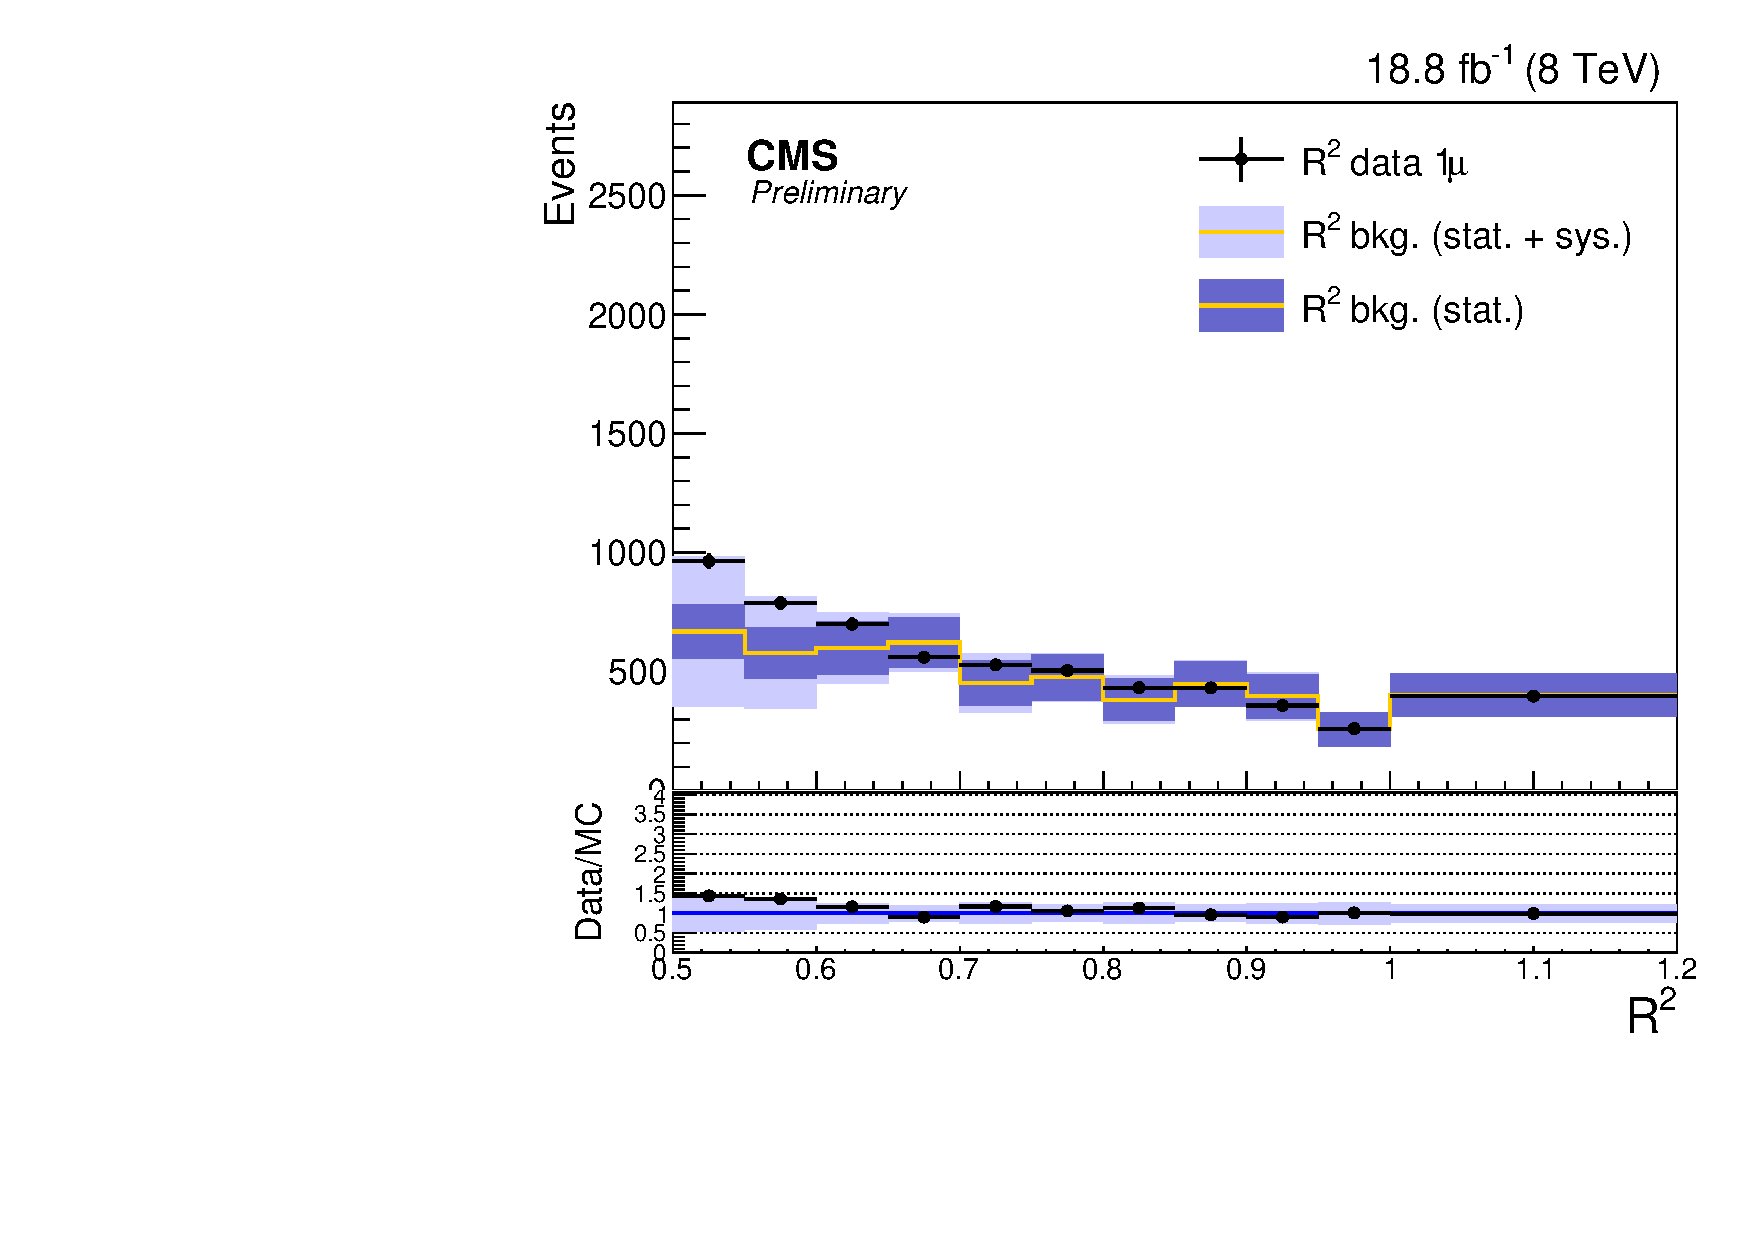
\includegraphics[width=0.45\textwidth]{DarkMatter8TeV/PredPlotsAN_1MU_LE/OneMu_sys_cat_1.pdf}  & 
   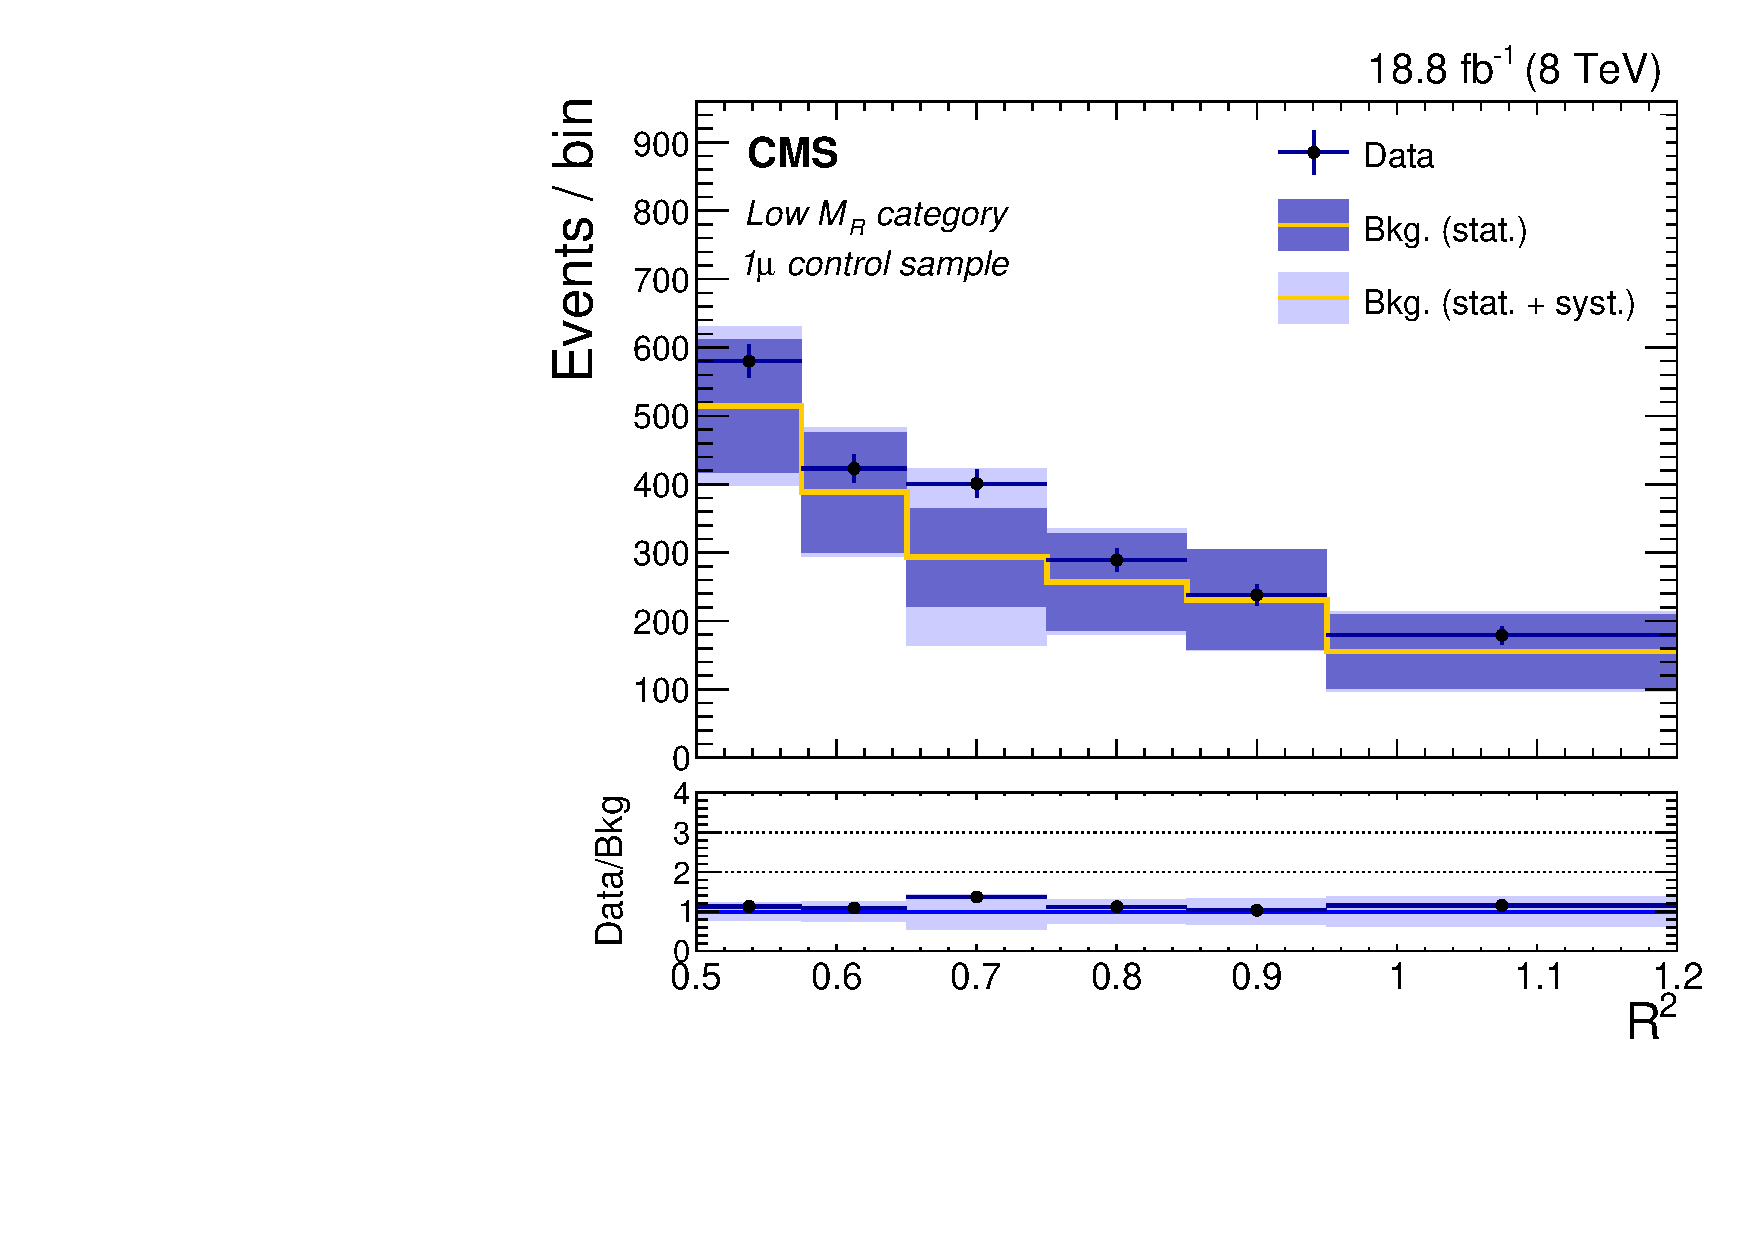
\includegraphics[width=0.45\textwidth]{DarkMatter8TeV/PredPlotsAN_1MU_LE/OneMu_sys_cat_2.pdf}
   \\
   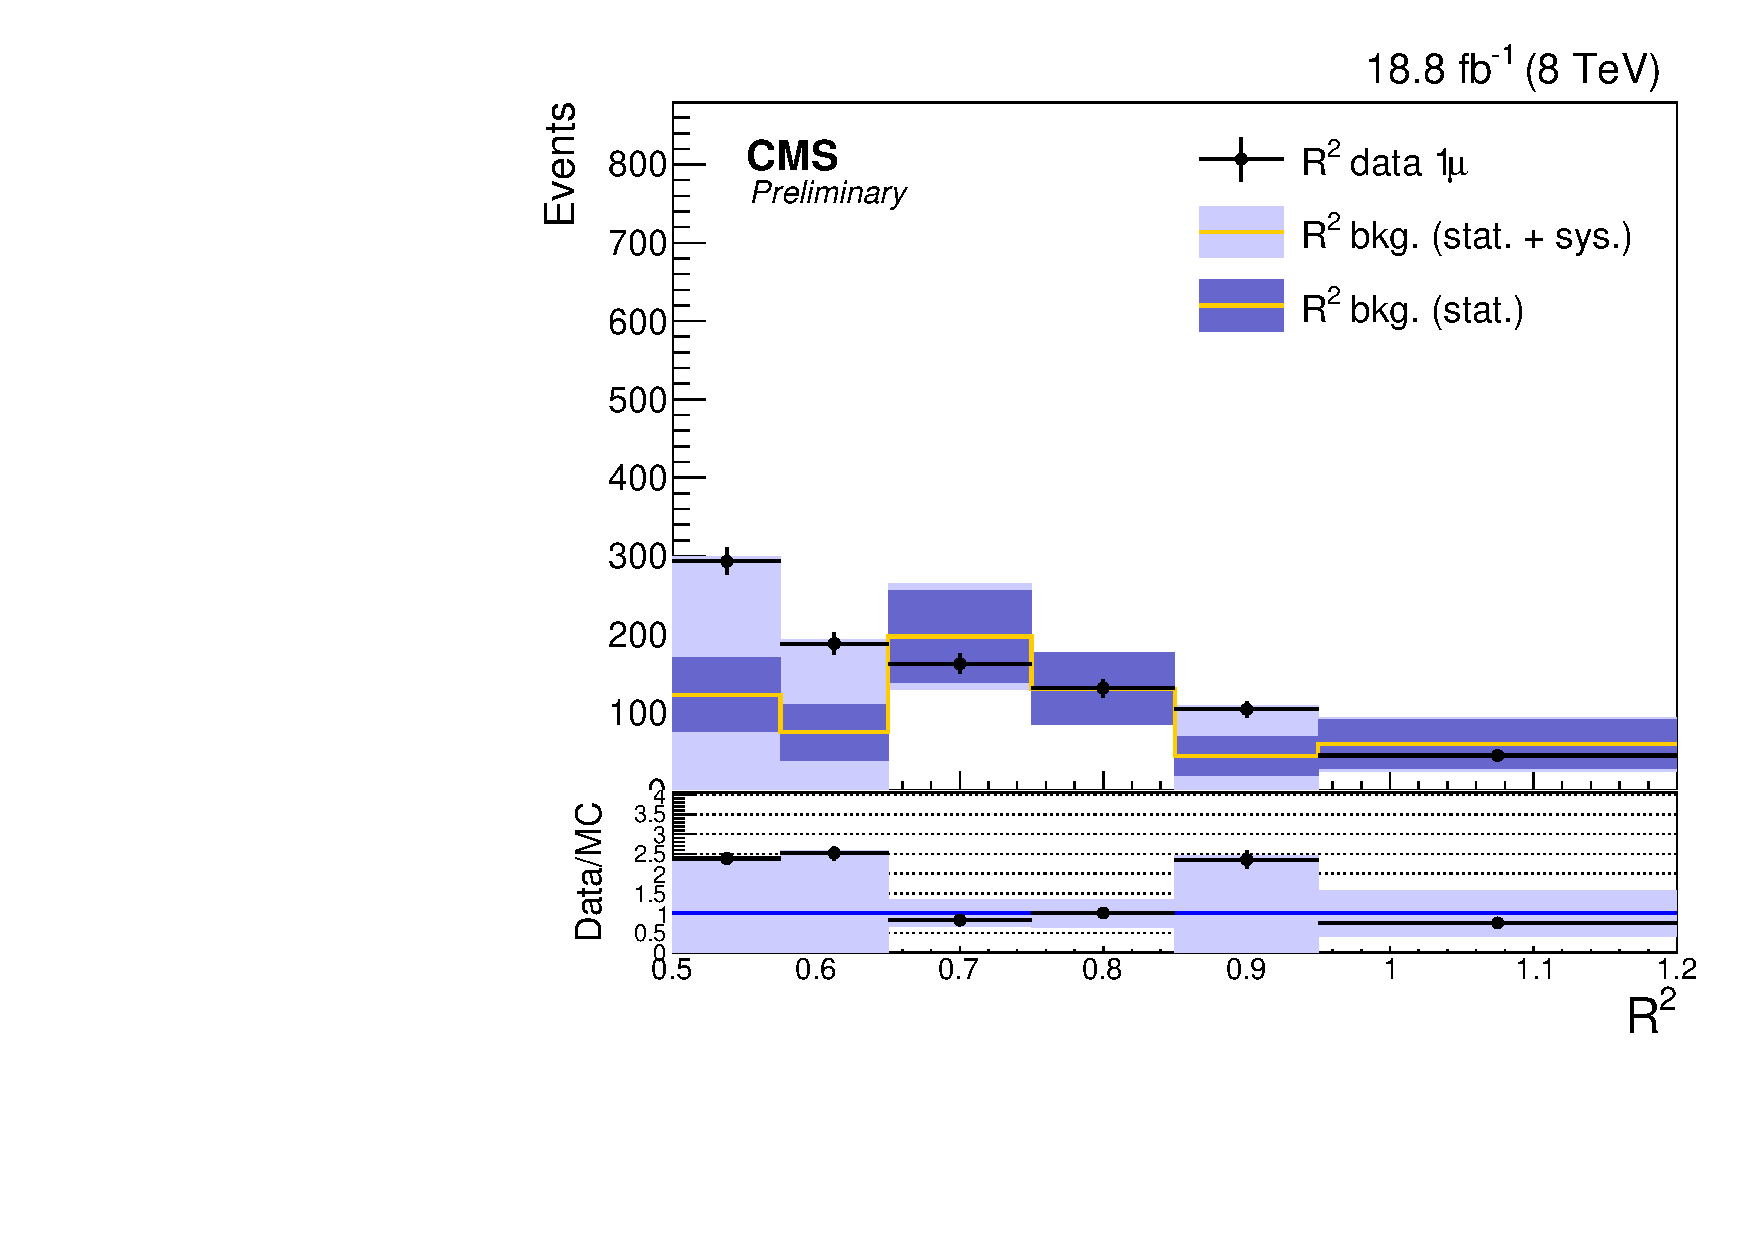
\includegraphics[width=0.45\textwidth]{DarkMatter8TeV/PredPlotsAN_1MU_LE/OneMu_sys_cat_3.pdf}  & 
   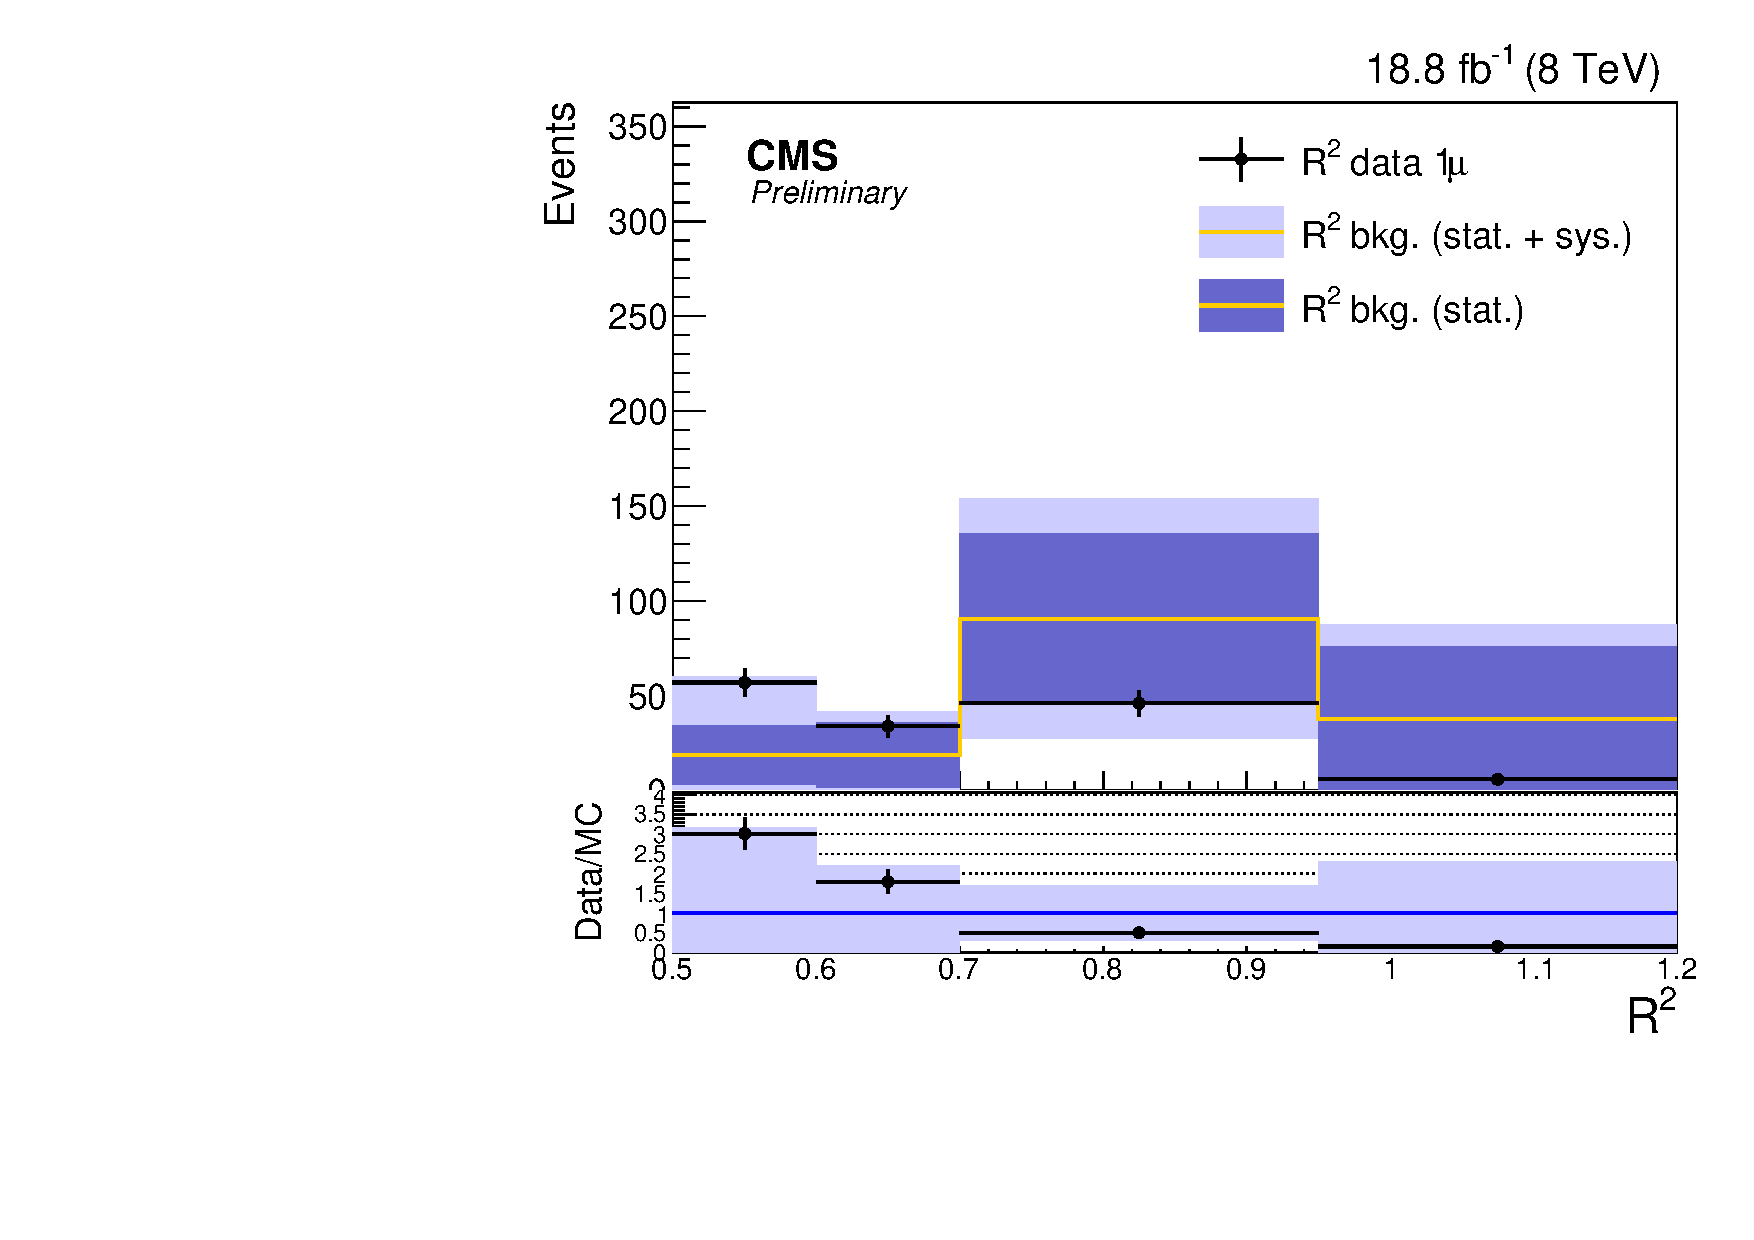
\includegraphics[width=0.45\textwidth]{DarkMatter8TeV/PredPlotsAN_1MU_LE/OneMu_sys_cat_4.pdf} \\
 \end{tabular}
 \caption{Comparison of observed yields in the 1$\mu$ sample and the
   background estimates from the 2$\mu$ sample in the four $\mathrm{M_{\rm R}}$ categories:
   VL (top left), L (top right), H (bottom left), and VH (bottom right). The bottom panel in each plot shows the
   ratio between the two distributions. The observed bin-by-bin
   deviation from unity is taken as a measurement of the uncertainty
   associated to the background estimation for the 0$\mu$ sample. The
   dark and light bands represent the statistical and the total
   uncertainties in the estimates, respectively. The horizontal bars indicate 
the variable bin widths.\label{fig:1muCLOSURE}}
\end{figure}

The $\ttbar$ background is determined with simulated
events, scaled to the NNLO cross section~\cite{WatNNLO,ZatNNLO,TTbaratNNLO} and further corrected for an
observed deviation from unity in the ratio 
of yields obtained from data and from simulation, measured in each $\mathrm{R^2}$ bin
of the 2$\mu$b control sample. The contribution of each  process to
the 2$\mu$b sample, predicted from simulated samples, is given in
Table~\ref{tab:2mub}. The fraction of \ttbar events in the 2$\mu$b
control sample is $\approx 95\%$. The observed yield is also
quoted. 
\begin{table}[h!]
  \caption{\label{tab:2mub} Observed yield and predicted
    background from simulated
    samples in the 2$\mu$b control sample. The quoted uncertainty in
    the prediction reflects the size of the simulated sample. The
    contribution of each individual background process is also shown,
    as estimated from simulated samples.}
\small
\centering
\begin{tabular}{|c|c|c|c|c|c|c|} 
  \hline
  Sample  &  $\cPZ(\nu \bar \nu)$+jets  &  $\PW(\ell \nu)$+jets  &
  $\cPZ(\ell \ell)$+jets  &  $\ttbar$  & MC predicted &  Observed \\
  \hline
  2$\mu$b  &   $<0.1$  & 0.1 $\pm$ 0.1 & 2.2 $\pm$ 0.3 & 58 $\pm$ 2 & 60 $\pm$ 2 & 60\\
  \hline
\end{tabular}
\end{table}
Figure~\ref{fig:2mub} shows the comparison of the observed
yield and the prediction from simulation, as a function of
$\mathrm{R^2}$. The uncertainty derived from the data-to-simulation ratio is
propagated to the systematic uncertainty in the $\ttbar$ prediction in
the 0$\mu$ search region. This $\mathrm{R^2}$-dependent factor and its
uncertainty account for possible systematic errors in the overall normalization, 
as might arise for instance from a systematic error in the theoretical cross section or in the estimate of the selection acceptance.

\begin{figure}[h!]
  \centering
   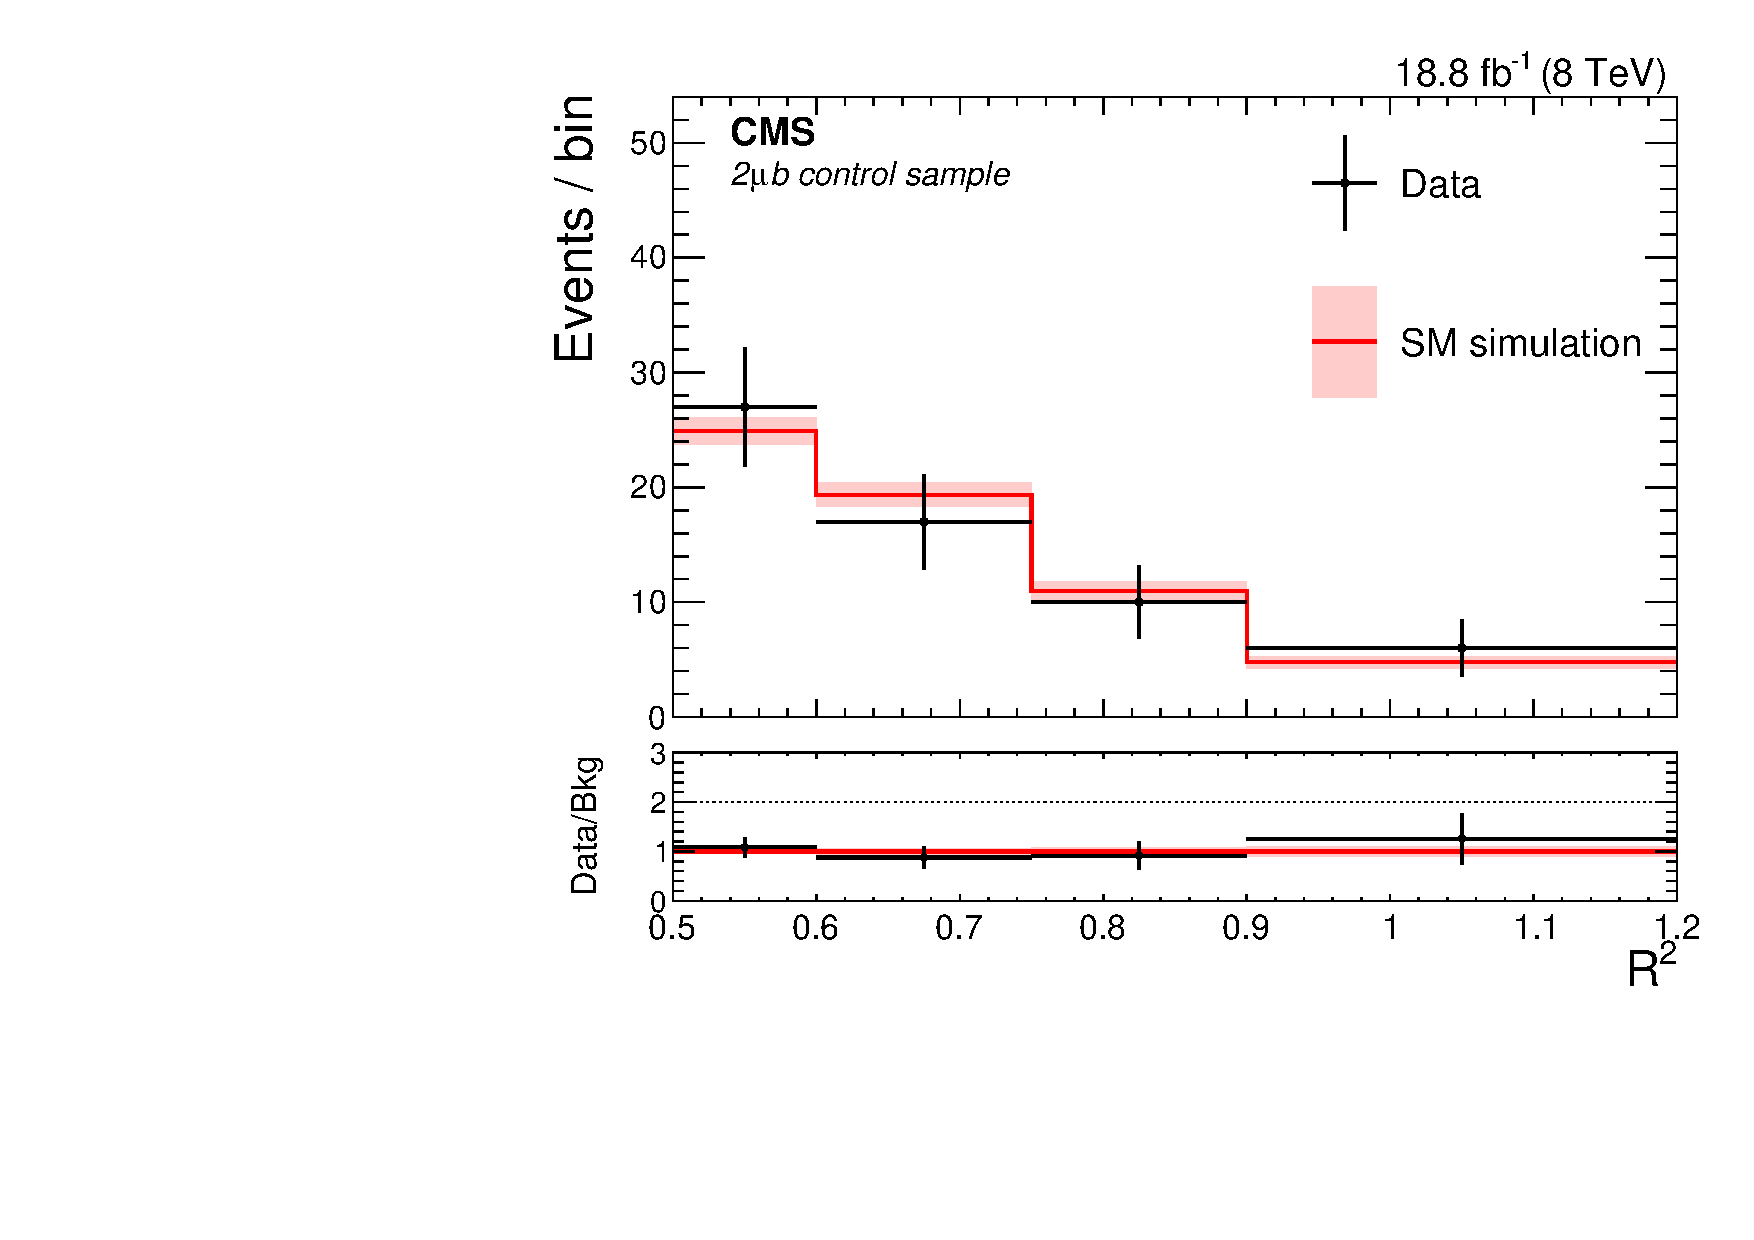
\includegraphics[width=0.5\textwidth]{DarkMatter8TeV/BtagPlots/MC_CP_2Mu1TbTT_Sep.pdf}
   \caption{Comparison of the observed yield and the prediction from
     simulation as a function of $\mathrm{R^2}$ in the 2$\mu$b control
     sample. The uncertainties in the data and the simulated
     sample are represented by the vertical bars and the shaded band,
     respectively. The horizontal bars indicate 
the variable bin widths.\label{fig:2mub}}
\end{figure}
The result of the background estimation is given in
Table~\ref{tab:bkg0mu}, where it is compared to the observed yields in
data. The uncertainty in the background estimates takes into account
both the statistical and systematic components. The contribution of each process is also given,
as predicted directly by simulated samples and therefore not used in
the final result.
%In the table, the yield expected from simulation is also quoted, computed using the NNLO
%production cross sections. The quoted uncertainty reflects the size of
%the simulated samples.

% \begin{table}
%  \centering
%  \caption{\label{tab:bkg0mu}  Comparison between the observed yield for 
%    0$\mu$ events in each $\mathrm{M_{\rm R}}$ category and the
%    corresponding estimation from background simulation and from
%    the data-driven method, using the 1$\mu$ sample. The uncertainty on
%    the data driven estimations take into account both the statistical 
%    and systematic uncertainty. The quoted uncertainty  in the
%    estimation from simulation reflects the size of the simulated sample.}
% \small
%  \begin{tabular}{|c|c|c|c|c|c|c|c|}
%   \hline
%   $\mathrm{M_{\rm R}}$  &  $\cPZ(\nu \bar \nu)$+jets  &  $\PW(
%   \ell \nu)$+jets  &  $\cPZ(\ell \ell)$+jets  &  $\ttbar$  &  Predicted  &  Predicted  &  Observed \\
% category &&&&& (simulation) & (data driven) & \\
%   \hline
%   VL  &  6231  $\pm$ 37  & 4820  $\pm$  33 & 49  $\pm$  2 & 555  $\pm$ 7 & 11655  $\pm$ 50 & 12773  $\pm$  899 & 11623 \\
%   L  &  2416 $\pm$ 19 & 1513 $\pm$ 16 & 11  $\pm$  1 & 104  $\pm$ 3  & 4044  $\pm$ 25  & 4165   $\pm$  265 & 3785 \\
%   H  &  1127 $\pm$  7 & 625 $\pm$  9 & 2.9  $\pm$ 0.3 & 24 $\pm$ 1 & 1778 $\pm$ 11 & 1654  $\pm$  686 & 1559 \\ 
%   VH  &  229  $\pm$ 2 & 103 $\pm$  3 & 0.2 $\pm$ 0.1 & 3.1 $\pm$ 0.5 & 335  $\pm$  4 & 243  $\pm$  156 & 261\\
%   \hline
% \end{tabular}
% \end{table}
\begin{table}[h!]
 \caption{\label{tab:bkg0mu}  Comparison of the observed yield for 
   0$\mu$ events in each $\mathrm{M_{\rm R}}$ category and the
   corresponding background estimates, using the 1$\mu$ sample. The uncertainty in
    the estimates takes into account both the statistical 
    and systematic components. The contribution of each individual background process is also shown, as 
estimated from simulated samples, as well as the total MC predicted yield.}
\small
\centering
 \begin{tabular}{|c|c|c|c|c|c|c|c|}
  \hline
  $\mathrm{M_{\rm R}}$  &  $\cPZ(\nu \bar \nu)$+jets  &  $\PW(
  \ell \nu)$+jets  &  $\cPZ(\ell \ell)$+jets  &  $\ttbar$  & MC predicted&  Estimated  &  Observed \\
category &&&&&& & \\
  \hline
  VL  &  6231  $\pm$ 37  & 4820  $\pm$  33 & 49  $\pm$  2 & 555  $\pm$
  7 & 11655 $\pm$ 50 &12770  $\pm$  900 & 11623 \\
  L  &  2416 $\pm$ 19 & 1513 $\pm$ 16 & 11  $\pm$  1 & 104  $\pm$ 3 & 4044 $\pm$ 25 & 4170   $\pm$  270 & 3785 \\
  H  &  1127 $\pm$  7 & 625 $\pm$  9 & 2.9  $\pm$ 0.3 & 24 $\pm$ 1  &  1779 $\pm$ 12 & 1650  $\pm$  690 & 1559 \\ 
  VH  &  229  $\pm$ 2 & 103 $\pm$  3 & 0.2 $\pm$ 0.1 & 3.1 $\pm$ 0.5 &
   335 $\pm$ 3 & 240  $\pm$  160 & 261\\
  \hline
\end{tabular}
\end{table}

The comparison of the data estimates and the observations for
each $\mathrm{M_{\rm R}}$ category is shown in
Fig.~\ref{fig:0muSignalBkg1GeV}, as a function of $\mathrm{R^2}$. For
completeness, the expected event distribution is shown for two signal
benchmark models, corresponding to the pair production of DM particles
of mass 1~GeV in the effective field theory (EFT) approach with vector coupling to u or d quarks. Details on the signal benchmark models are
given in Section~\ref{sec:EFT0mu}.

%\begin{figure}[ht!]
% \centering
% \begin{tabular}{cc}
%  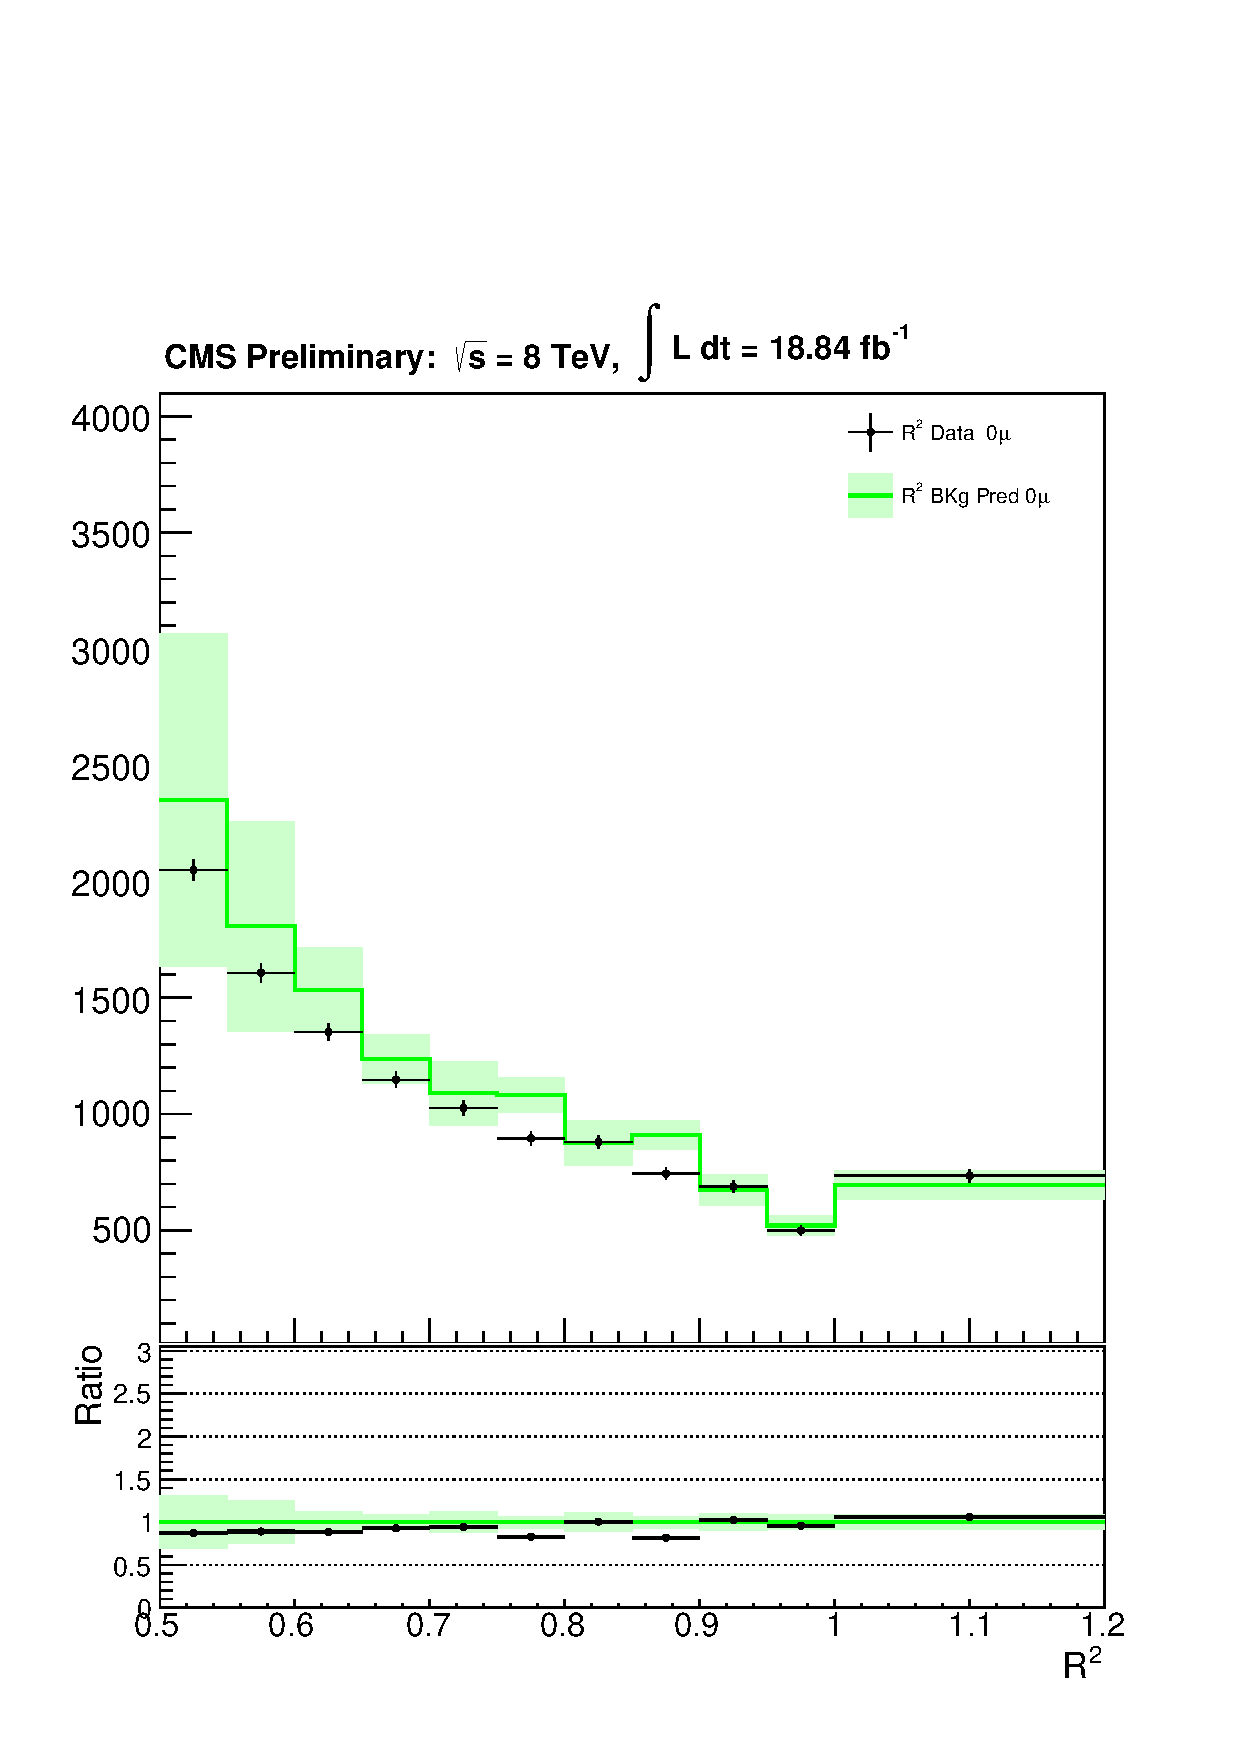
\includegraphics[width=0.35\textwidth]{PredPlotsAN/Bkg_R2_0mu_0b_Pred_SYS_cat1_NEW_kF.pdf}  & 
%   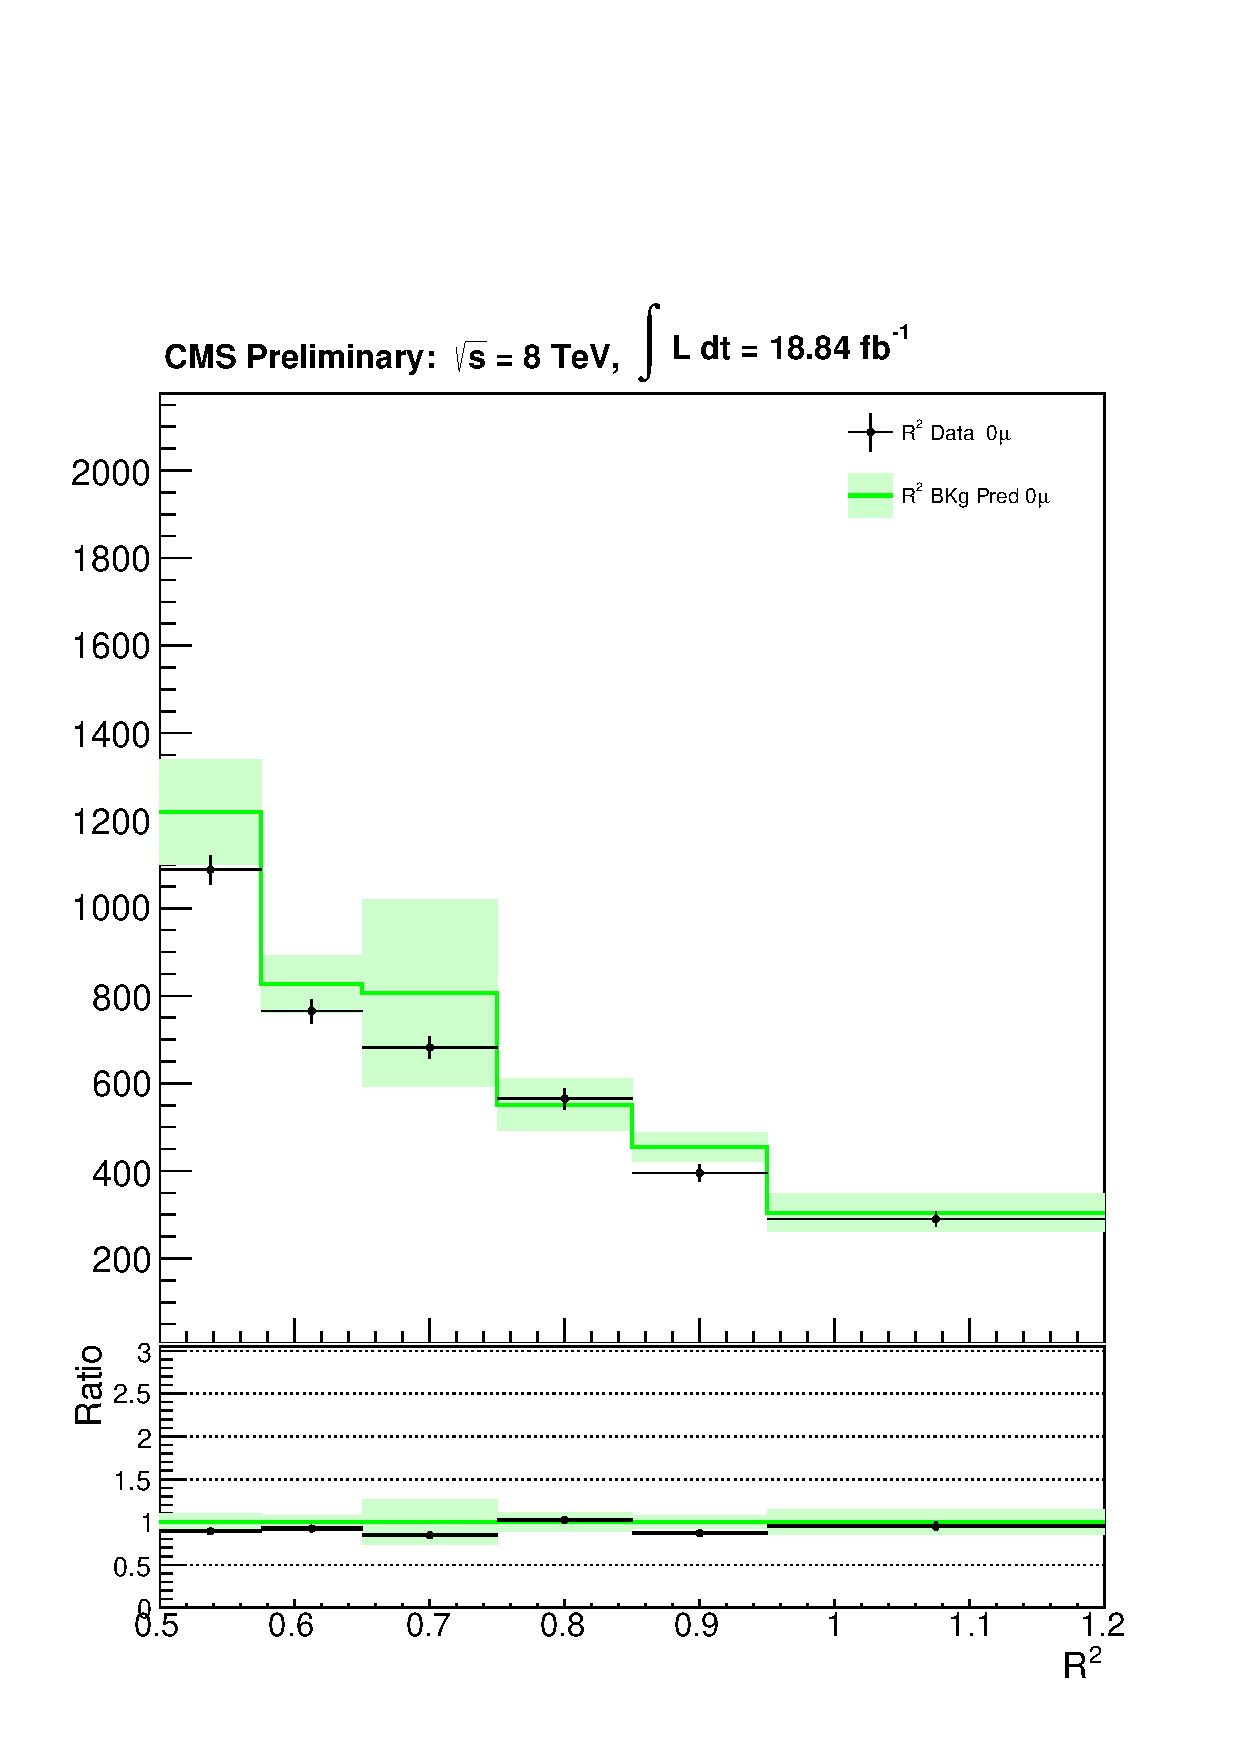
\includegraphics[width=0.35\textwidth]{PredPlotsAN/Bkg_R2_0mu_0b_Pred_SYS_cat2_NEW_kF.pdf} \\
%   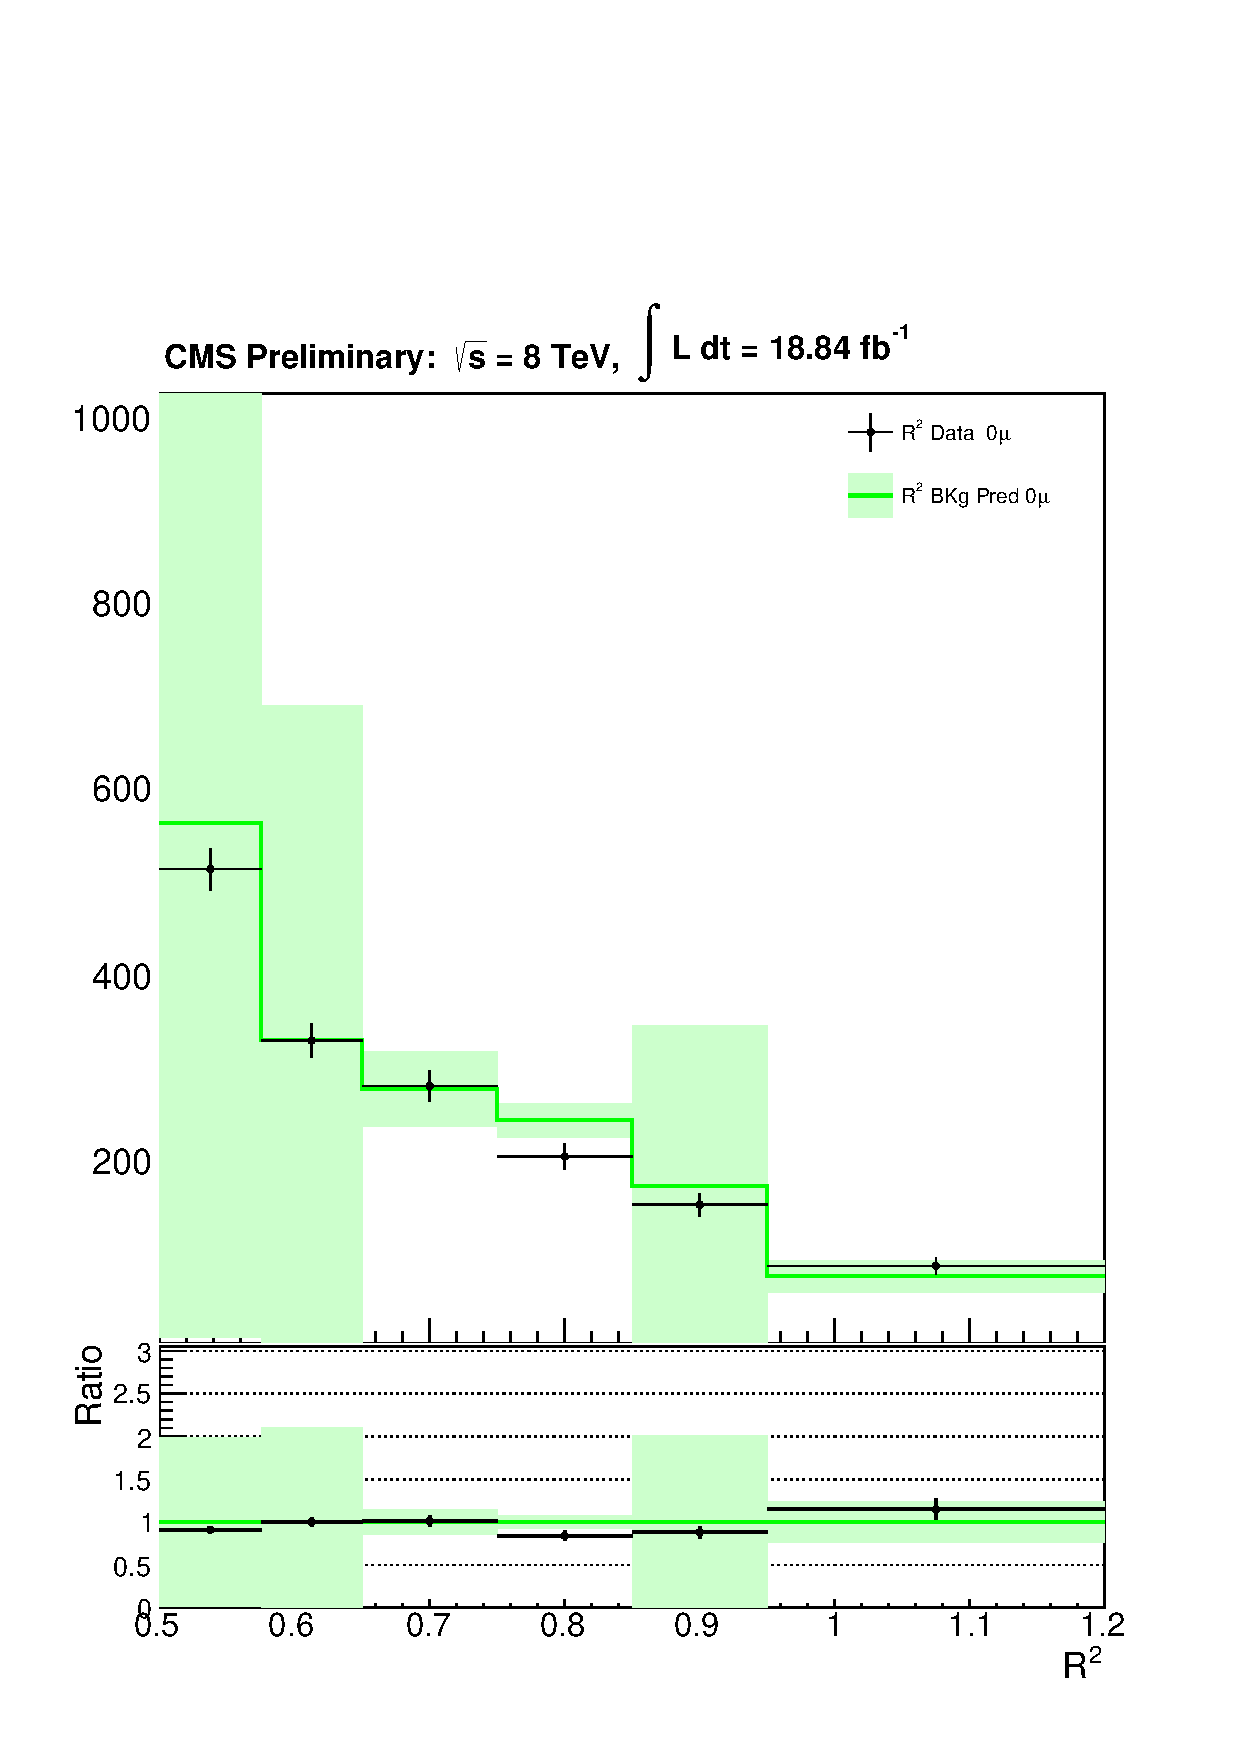
\includegraphics[width=0.35\textwidth]{PredPlotsAN/Bkg_R2_0mu_0b_Pred_SYS_cat3_NEW_kF.pdf}  & 
%   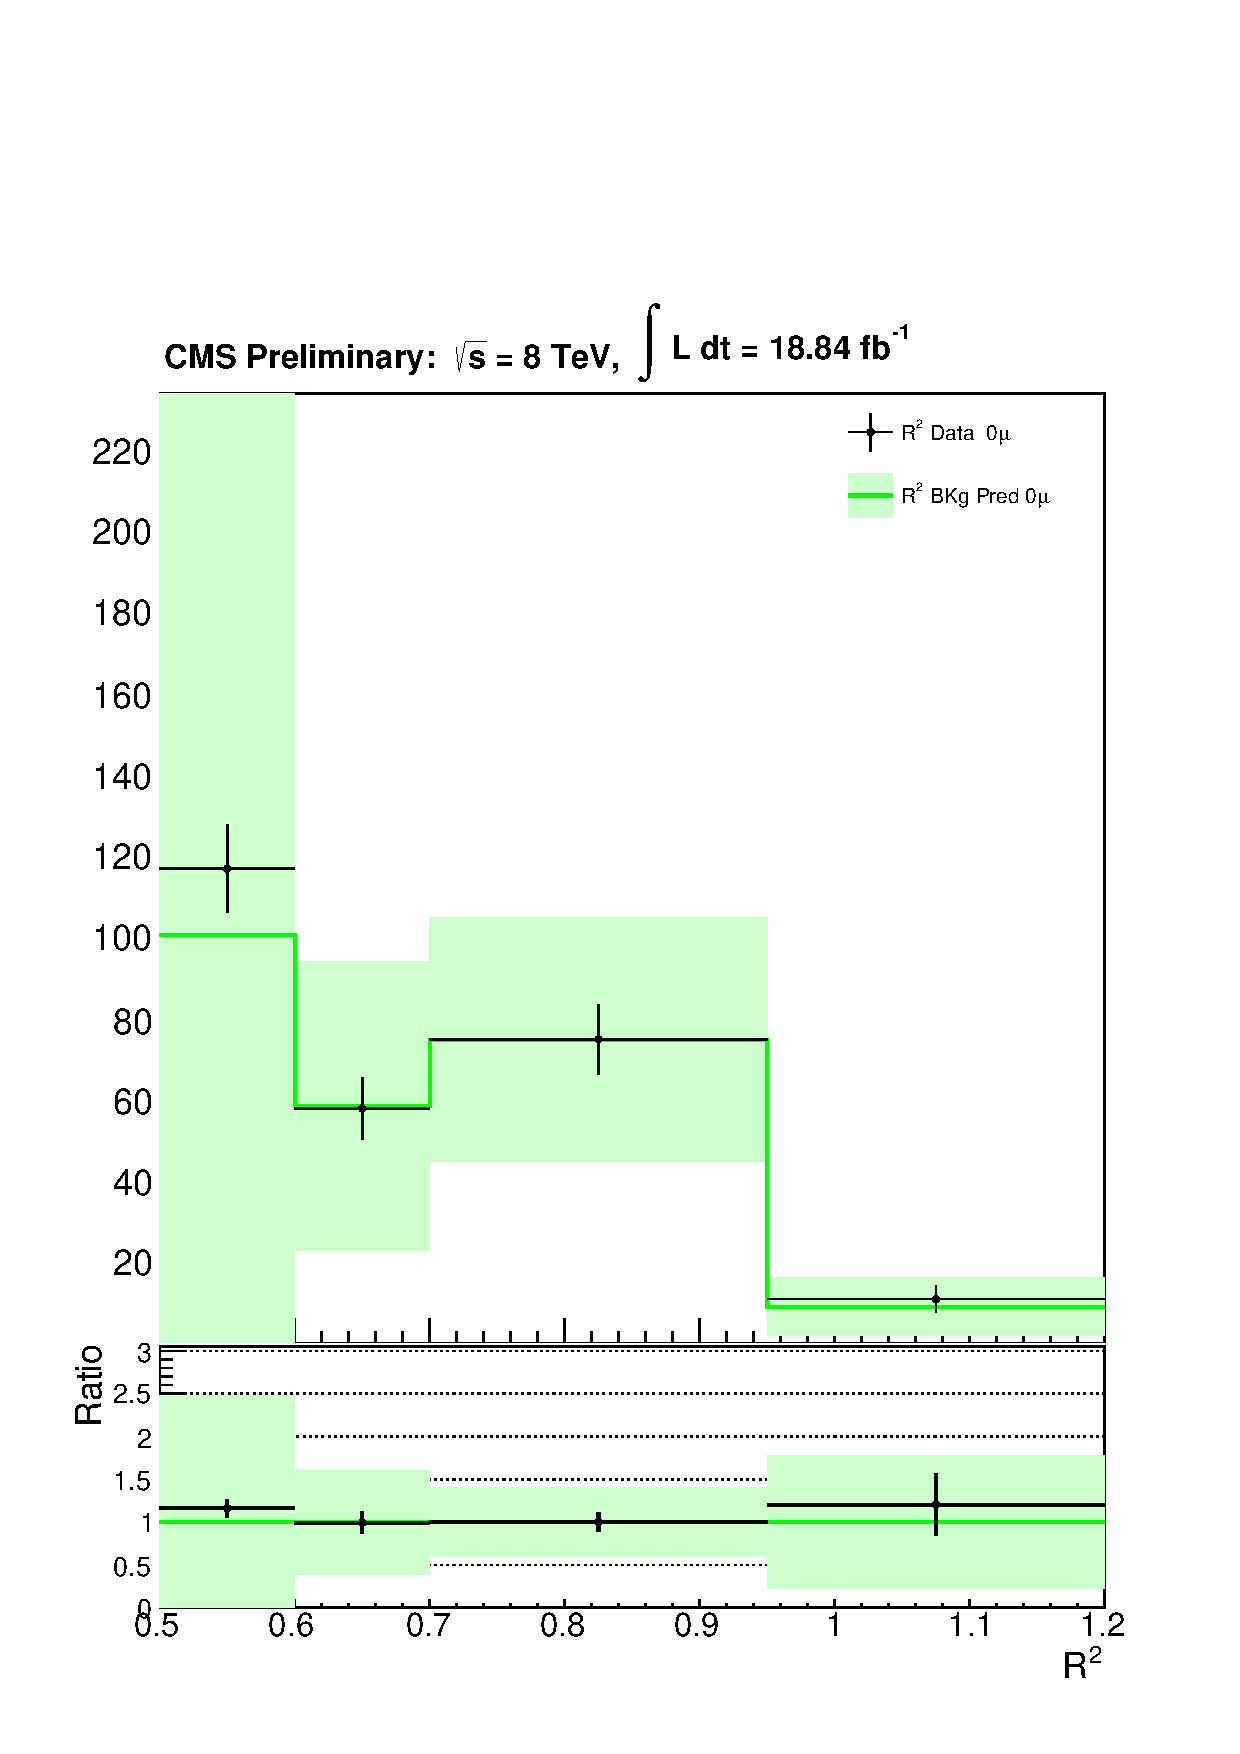
\includegraphics[width=0.35\textwidth]{PredPlotsAN/Bkg_R2_0mu_0b_Pred_SYS_cat4_NEW_kF.pdf} 
% \end{tabular}
% \caption{Comparison of observed yield in the 0-$\mu$ sample and the
%   data-driven estimation from the 1-$\mu$ and 2-$\mu$ sample.  The
%   bottom panels show the ratio between the two
%   distributions.\label{fig:0muSignalRegion}}
%\end{figure}

\begin{figure}[h!]
 \centering
 \begin{tabular}{cccc}
   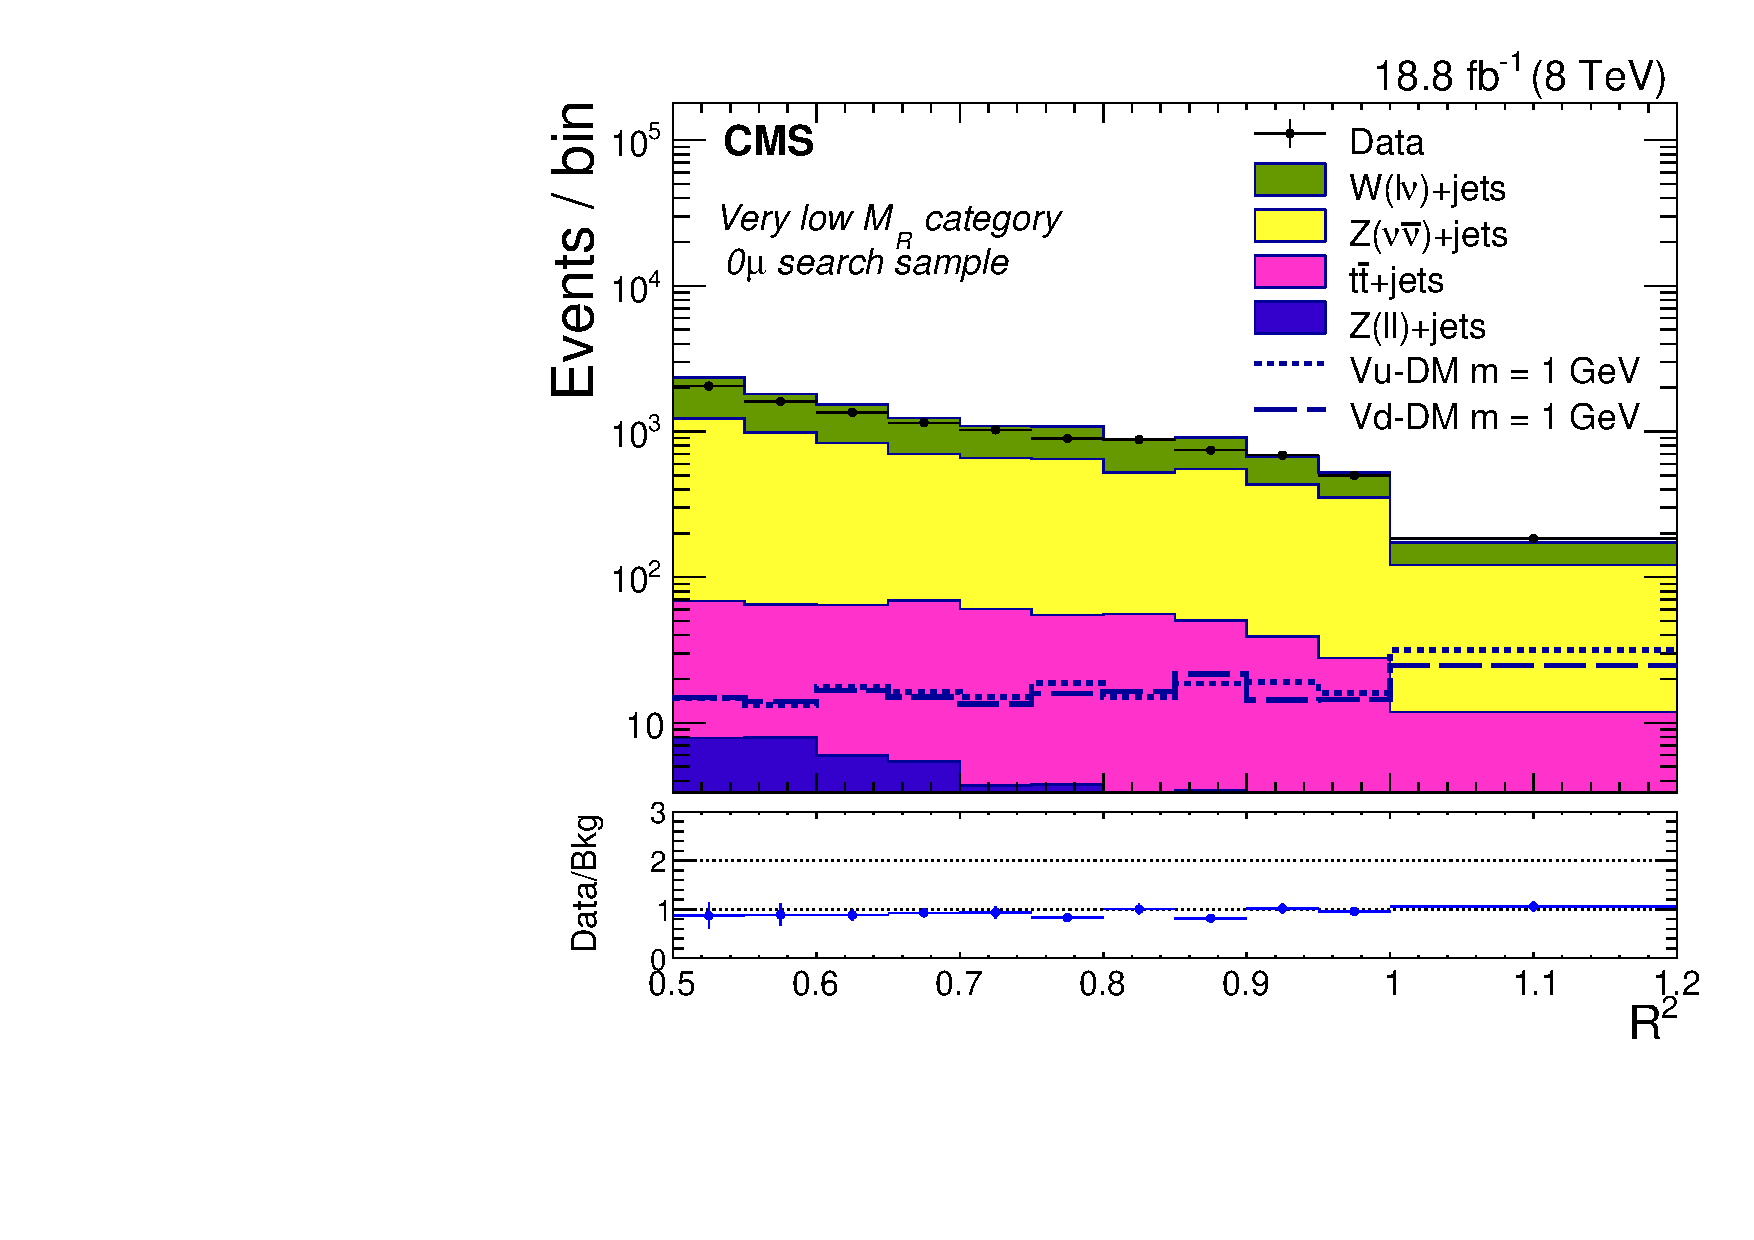
\includegraphics[width=0.5\textwidth]{DarkMatter8TeV/SignalBkgPlots/Data_MC_cat1_1_DoubleSignal_V.pdf}  & 
   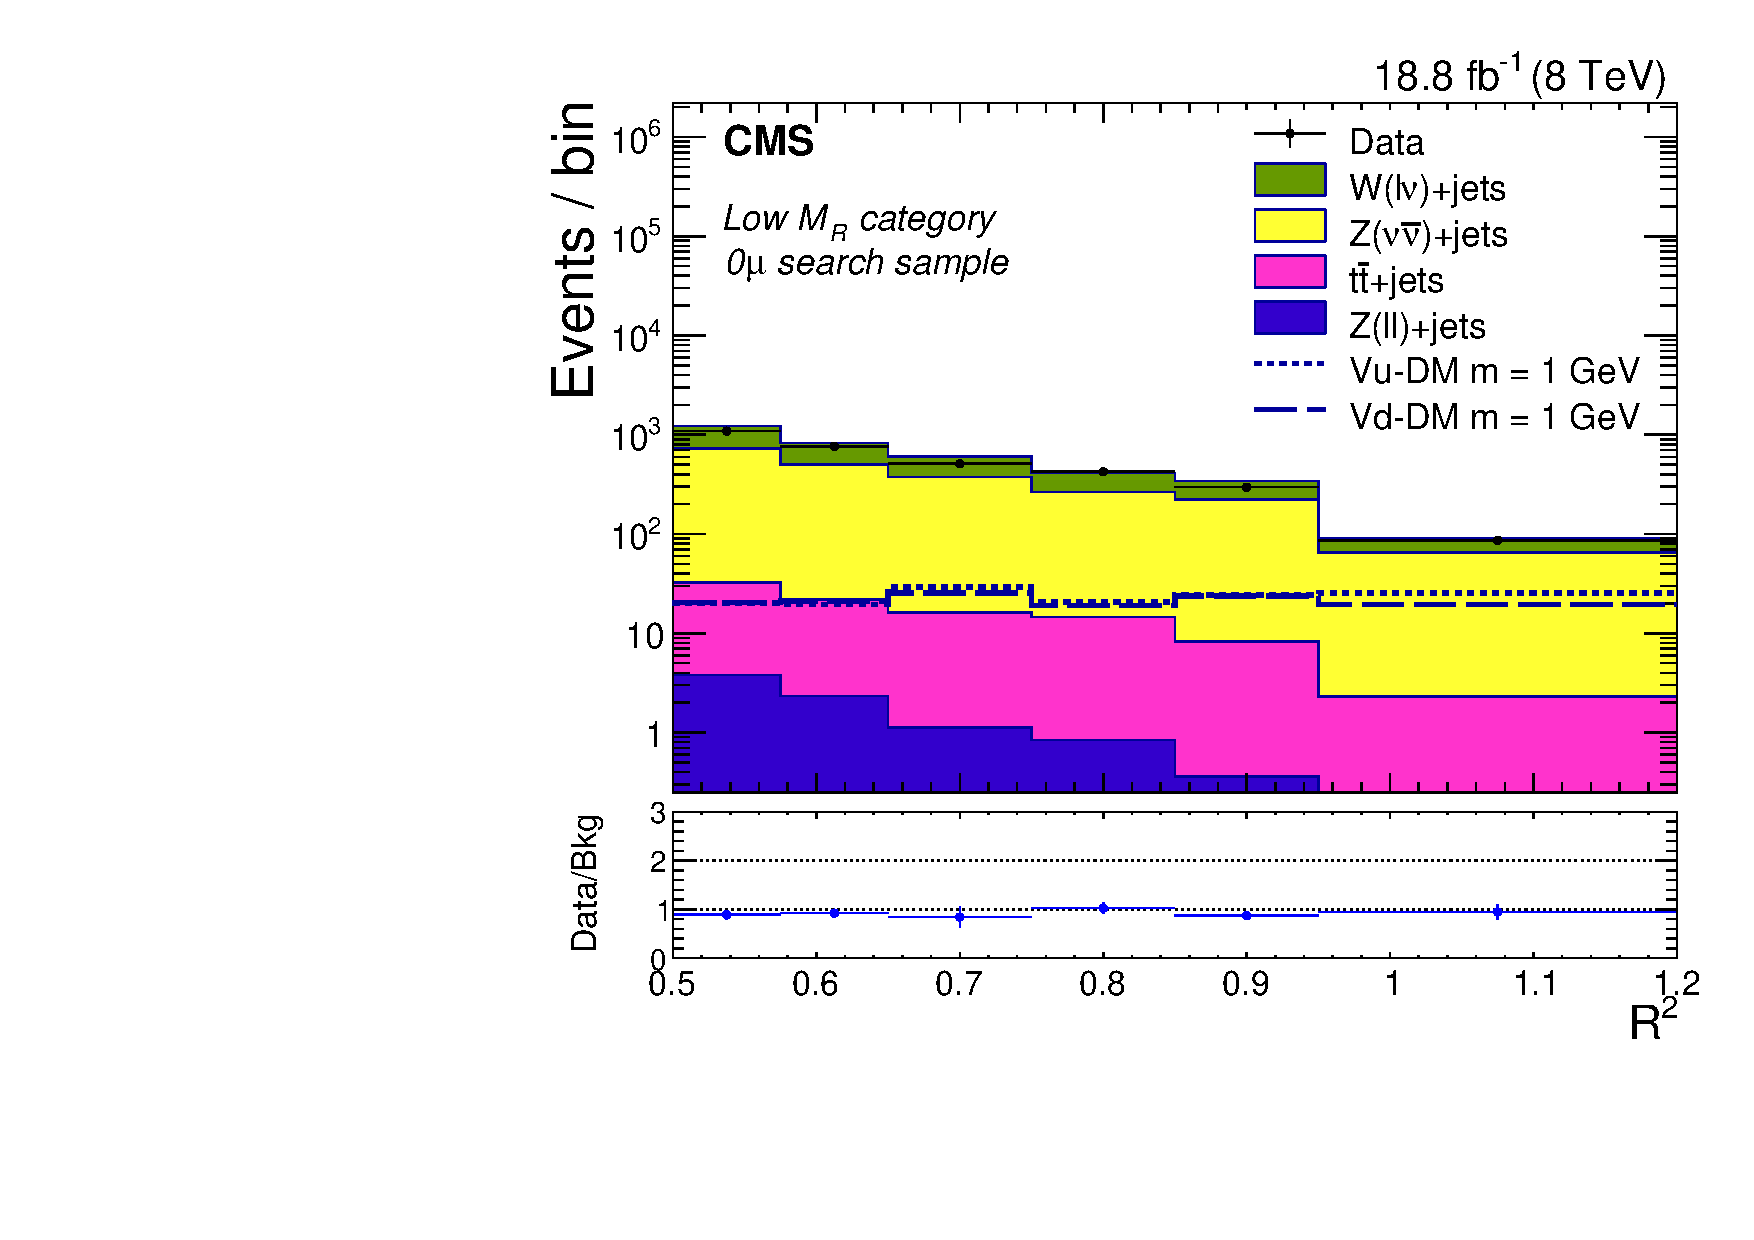
\includegraphics[width=0.5\textwidth]{DarkMatter8TeV/SignalBkgPlots/Data_MC_cat2_1_DoubleSignal_V.pdf} \\ 
   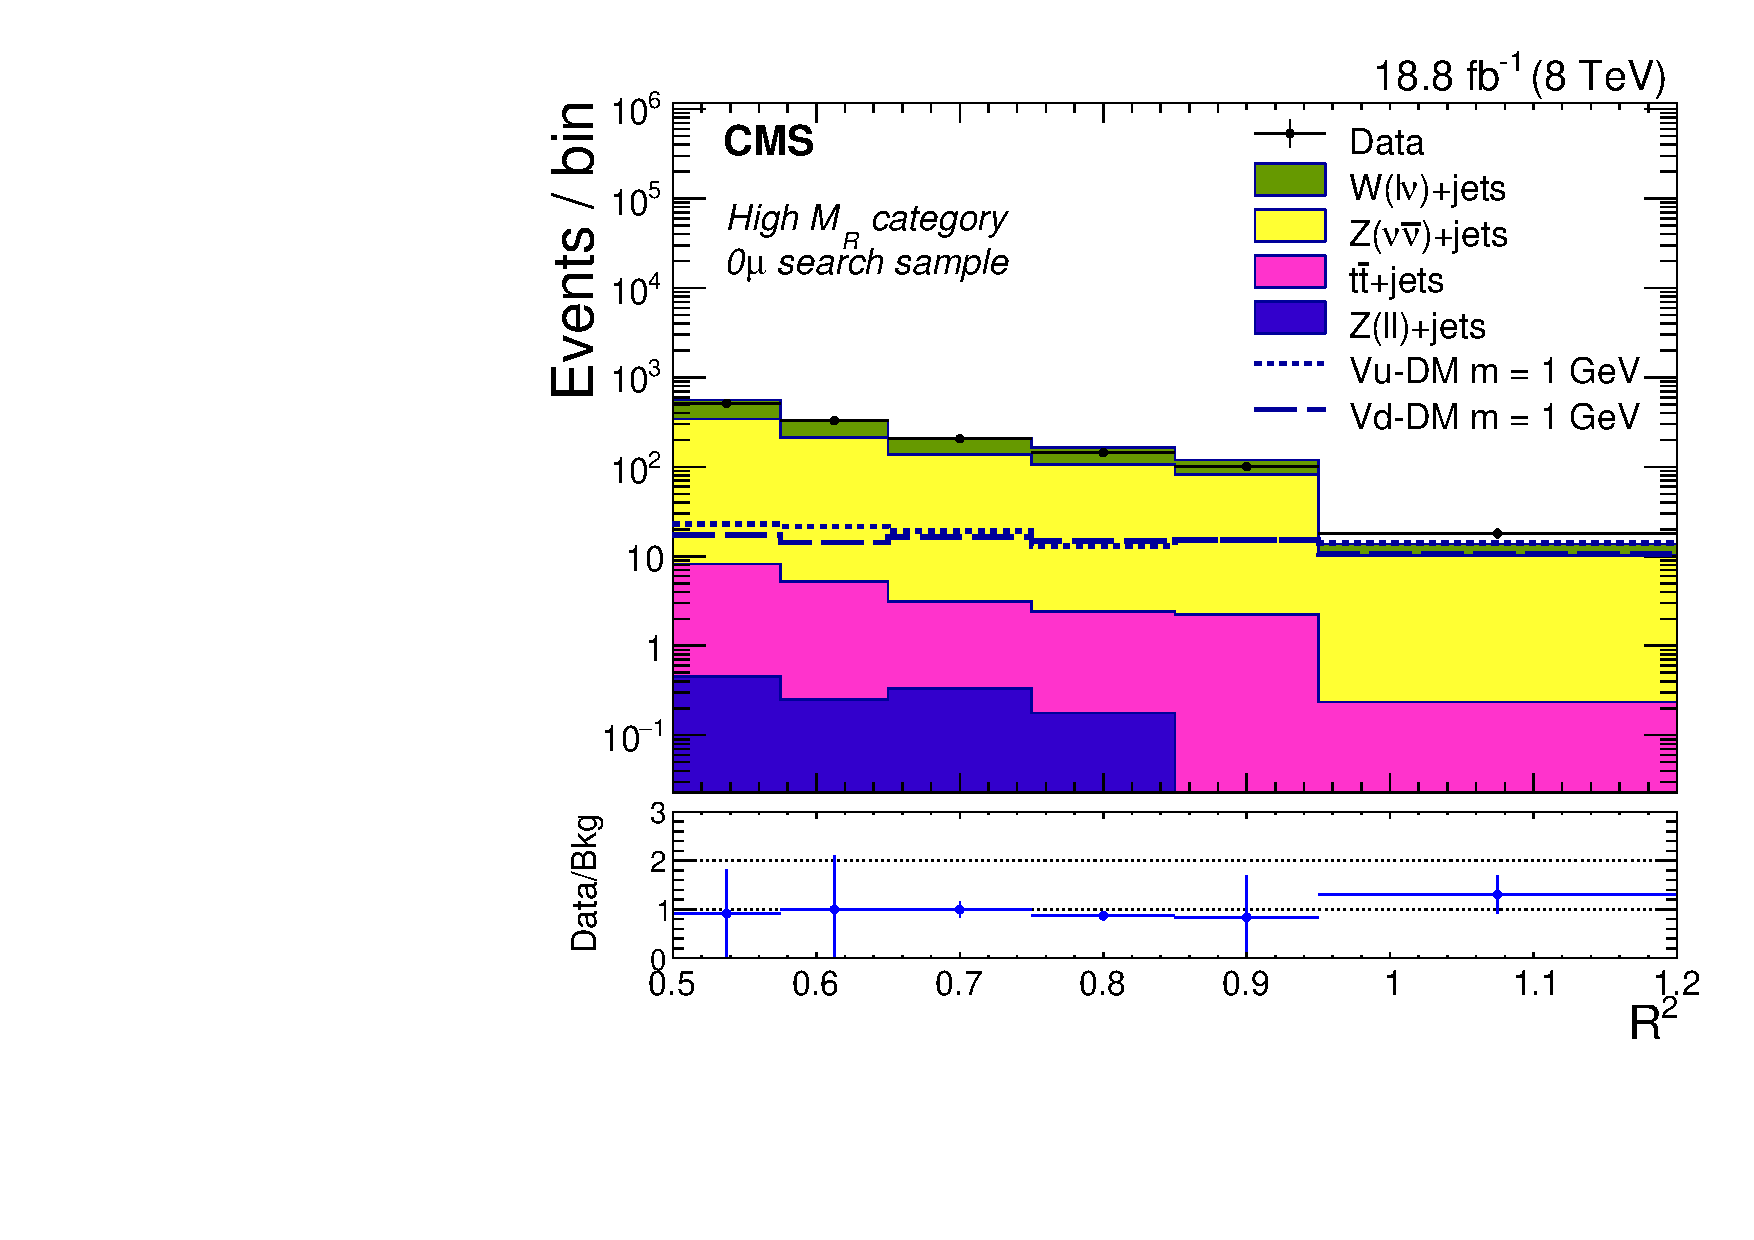
\includegraphics[width=0.5\textwidth]{DarkMatter8TeV/SignalBkgPlots/Data_MC_cat3_1_DoubleSignal_V.pdf}  & 
   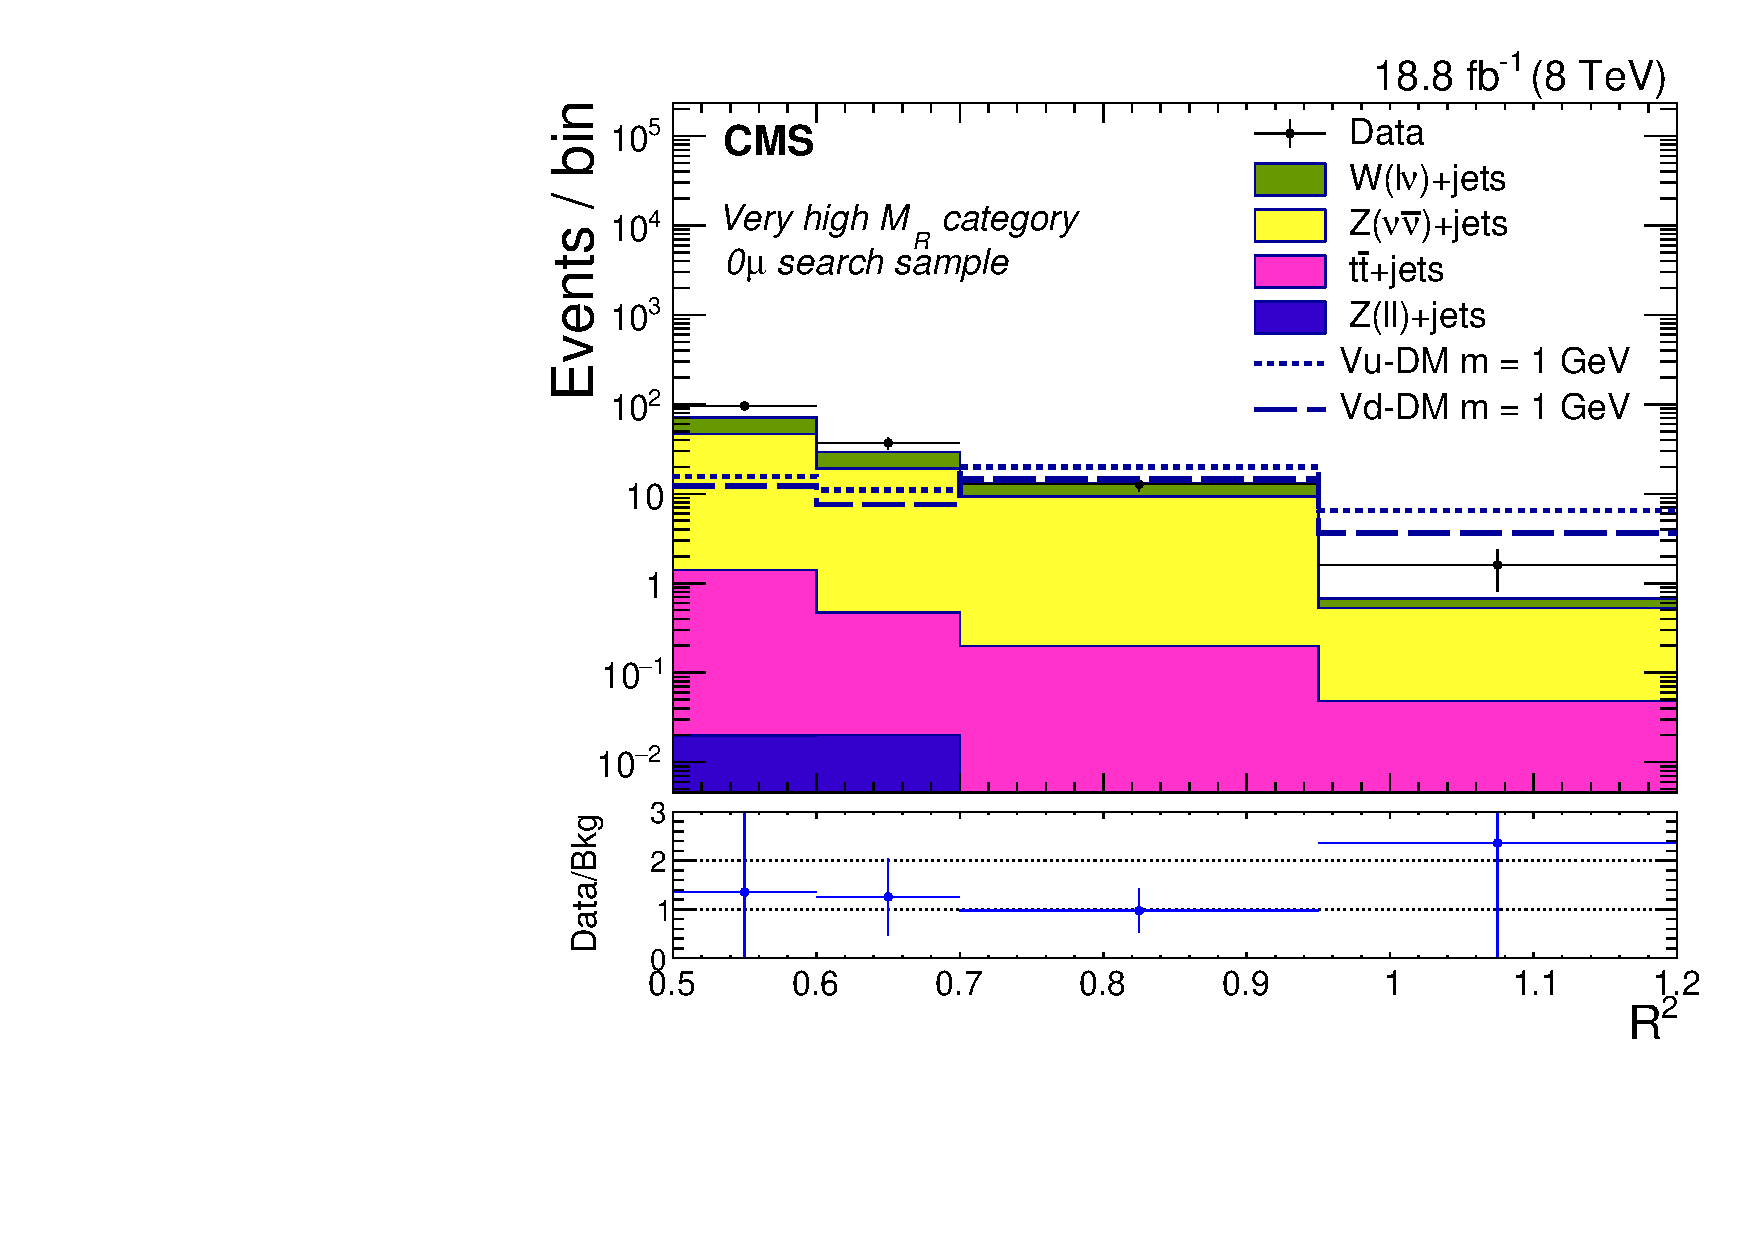
\includegraphics[width=0.5\textwidth]{DarkMatter8TeV/SignalBkgPlots/Data_MC_cat4_1_DoubleSignal_V.pdf}\\
 \end{tabular}
 \caption{Comparison of the observed yield in the $0\mu$ sample and the
   background estimates in the four $\mathrm{M_{\rm R}}$ categories:
   VL (top left), L (top right), H (bottom left), and VH (bottom right). The
   contribution of individual background processes is shown by the
   filled histograms. The bottom panels show the ratio
   between the observed yields and the total background estimate. For reference, the distributions from two
   benchmark signal models are also shown, corresponding to the pair
   production of DM particles of mass 1 \GeV in the EFT approach with
   vector coupling to u or d quarks. The horizontal bars indicate 
the variable bin widths.\label{fig:0muSignalBkg1GeV} }
\end{figure}

\subsection{Background estimation for the 0$\mu$b and 0$\mu$bb samples}
A technique similar to that described in Section 6.1 is used to determine the
expected background for the 0$\mu$b and the 0$\mu$bb samples.

The background from $\ttbar$ events for each $\mathrm{R^2}$ bin in the
0$\mu$b sample, $n(\ttbar)_{i}^{0\mu\mathrm{b}}$, is computed as:
% \begin{equation}
%   n(\ttbar)_{i}^{0\mu\mathrm{b}} =  n(\ttbar)_{i}^{2\mu\mathrm{b}}
%   \frac{N(\ttbar)_{i}^{0\mu\mathrm{b}}}{N(\ttbar)_{i}^{2\mu\mathrm{b}}}\label{eq:bBkgPred}
% \end{equation}

\begin{equation}
  n(\ttbar)_{i}^{0\mu\mathrm{b}} =  (n(\ttbar)_{i}^{2\mu\mathrm{b}} - N_{i}^{Z(\ell
    \ell)+\mathrm{jets},2\mu\mathrm{b}} - N_{i}^{W(\ell\nu)+\mathrm{jets},2\mu\mathrm{b}})
\frac{N(\ttbar)_{i}^{0\mu\mathrm{b}}}{N(\ttbar)_{i}^{2\mu\mathrm{b}}}\label{eq:bBkgPred}
\end{equation}

where $n(\ttbar)_{i}^{2\mu\mathrm{b}}$ is the observed yield in the $\math{i}$th $\mathrm{R^2}$
bin for the 2$\mu$b sample, while $N(\ttbar)_{i}^{0\mu\mathrm{b}}$ and
$N(\ttbar)_{i}^{2\mu\mathrm{b}}$ are, respectively, the corresponding $\ttbar$ yields in the $\math{i}$th $\mathrm{R^2}$
bin for the 0$\mu$b and 2$\mu$b samples derived from
the simulated \ttbar sample. Similarly, the \ttbar background in the
0$\mu$bb sample is derived from Eq. (\ref{eq:bBkgPred}), replacing
$N(\ttbar)_{i}^{0\mu\mathrm{b}}$ with $N(\ttbar)_{i}^{0\mu\mathrm{bb}}$, the \ttbar
background yield in the $\math{i}$th bin of the 0$\mu$bb sample, predicted
from the simulated \ttbar events. The data yield in the 2$\mu$b sample is
corrected to account for the small contamination from $\cPZ$+jets and
 $\PW$+jets, predicted with the simulated yields $N_{i}^{Z(\ell
    \ell)+\mathrm{jets},2\mu\mathrm{b}$ and
    $N_{i}^{W(\ell\nu)+\mathrm{jets},2\mu\mathrm{b}}$, respectively.


The background contribution from $\PW(\ell \nu)$+jets and $\cPZ(\nu
\bar \nu)$+jets events is predicted using the $\cPZ(\mu\mu)$b sample,
having a $\cPZ$+jets purity $\approx 89\%$ (see
Table~\ref{tab:WITHB}). The observed yield in the $\cPZ(\mu\mu)$b
sample is shown in the left plot of Fig.~\ref{fig:Zmumub}, as a
function of $\mathrm{R^2}$. This contribution, scaled by the ratio of the predicted V+jets background in the signal region to that in the control sample, obtained from simulation; provides an
estimate for each $\mathrm{R^2}$ bin. In Table~\ref{tab:WITHB}  and
in the left plot of Fig.~\ref{fig:Zmumub}, discrepancies between the observation and the prediction could be
larger than the quoted uncertainty, since the latter accounts only for the
statistical uncertainty of the simulated sample.

% \begin{table}[htb]
%   \caption{\label{tab:WITHB} Expected background estimations
%     from simulation and observed yields for control samples
%     with b-tagged jets. When available, a data-driven background
%     estimation is also provided, derived as described in the text.}
% \small
% \begin{tabular}{|c|c|c|c|c|c|c|c|} 
%   \hline
%   Sample  &  $\cPZ(\nu \bar \nu)$+jets  &  $\PW(\ell \nu)$+jets  &
%   $\cPZ(\ell \ell)$+jets  &  $\ttbar$  &  Predicted   &  Predicted  &
%   Observed \\
% category &&&&& (simulation) & (data driven) & \\
%   \hline
%    $\cPZ(\mu\mu)$b  &  -  &  -  & 134 $\pm$ 3 & 17 $\pm$ 1 & 151 $\pm$  3 &  -  &  175 \\
%   \hline
%    $1\mu$b &  0.2 $\pm$ 0.1 & 279 $\pm$ 7 & 11 $\pm$  1 & 3038 $\pm$ 17 & 3328  $\pm$ 18 & 3405 $\pm$ 544 & 2920\\
%   \hline
% \end{tabular}
% \end{table}

\begin{table}[h!]
  \caption{\label{tab:WITHB} 
    %Comparison between (top row) the observed yield for
    %$\cPZ(\mu\mu)$b events and the corresponding
    %prediction from background simulation and (bottom row) the observed yield for
    %$1\mu$b events and the corresponding
    %background estimate. The quoted uncertainty in the
    %$\cPZ(\mu\mu)$b prediction reflects the size of the simulated sample, while the uncertainty on
    %the $1\mu$b estimate takes into account both the statistical and
    %systematic components.
    Comparison of the observed yields in the $\cPZ(\mu\mu)$b and
    $1\mu$b samples, the corresponding predictions from background
    simulation, and (for $1\mu$b only) the cross-check background
    estimate. The contribution of each individual background process is also shown, as 
estimated from simulated samples.
}
\small
\centering
\begin{tabular}{|c|c|c|c|c|c|c|c|} 
  \hline
  Sample  &  $\cPZ(\nu \bar \nu)$+jets  &  $\PW(\ell \nu)$+jets  &
  $\cPZ(\ell \ell)$+jets  &  $\ttbar$   &  MC predicted  & Estimated & 
  Observed \\
category &&&&& && \\
  \hline
   $\cPZ(\mu\mu)$b  &  $<0.1$  &  $<0.1$  & 134 $\pm$ 3 & 17 $\pm$ 1 &
   151 $\pm$ 3 & N/A  &  175 \\
  \hline
   $1\mu$b &  0.2 $\pm$ 0.1 & 279 $\pm$ 7 & 11 $\pm$  1 & 3038 $\pm$
   17 & 3328 $\pm$ 18 & 3410 $\pm$ 540 & 2920\\
  \hline
\end{tabular}
\end{table}

\begin{figure}[h!]
  \centering
  \begin{tabular}{cc}
   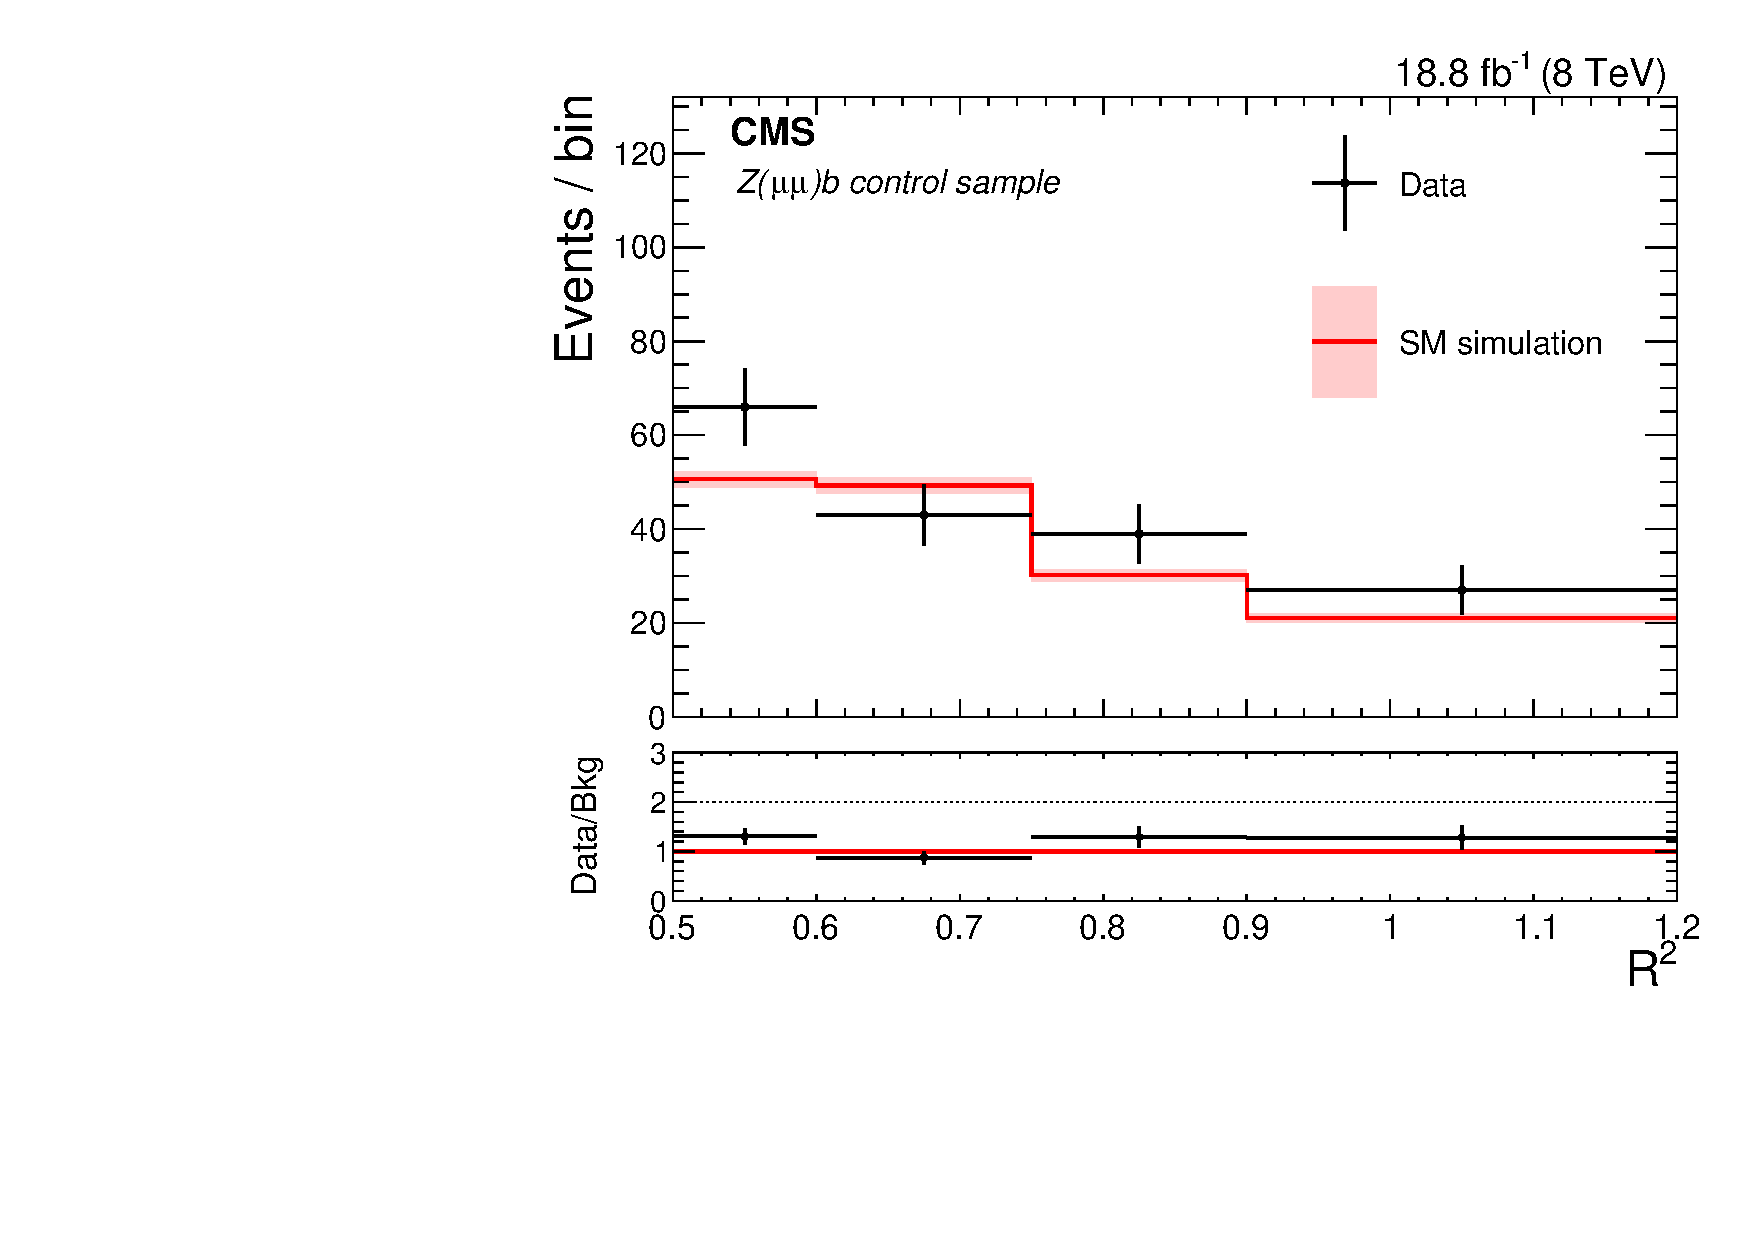
\includegraphics[width=0.5\textwidth]{DarkMatter8TeV/BtagPlots/MC_CP_2Mu1LbZ_Sep.pdf}  & 
   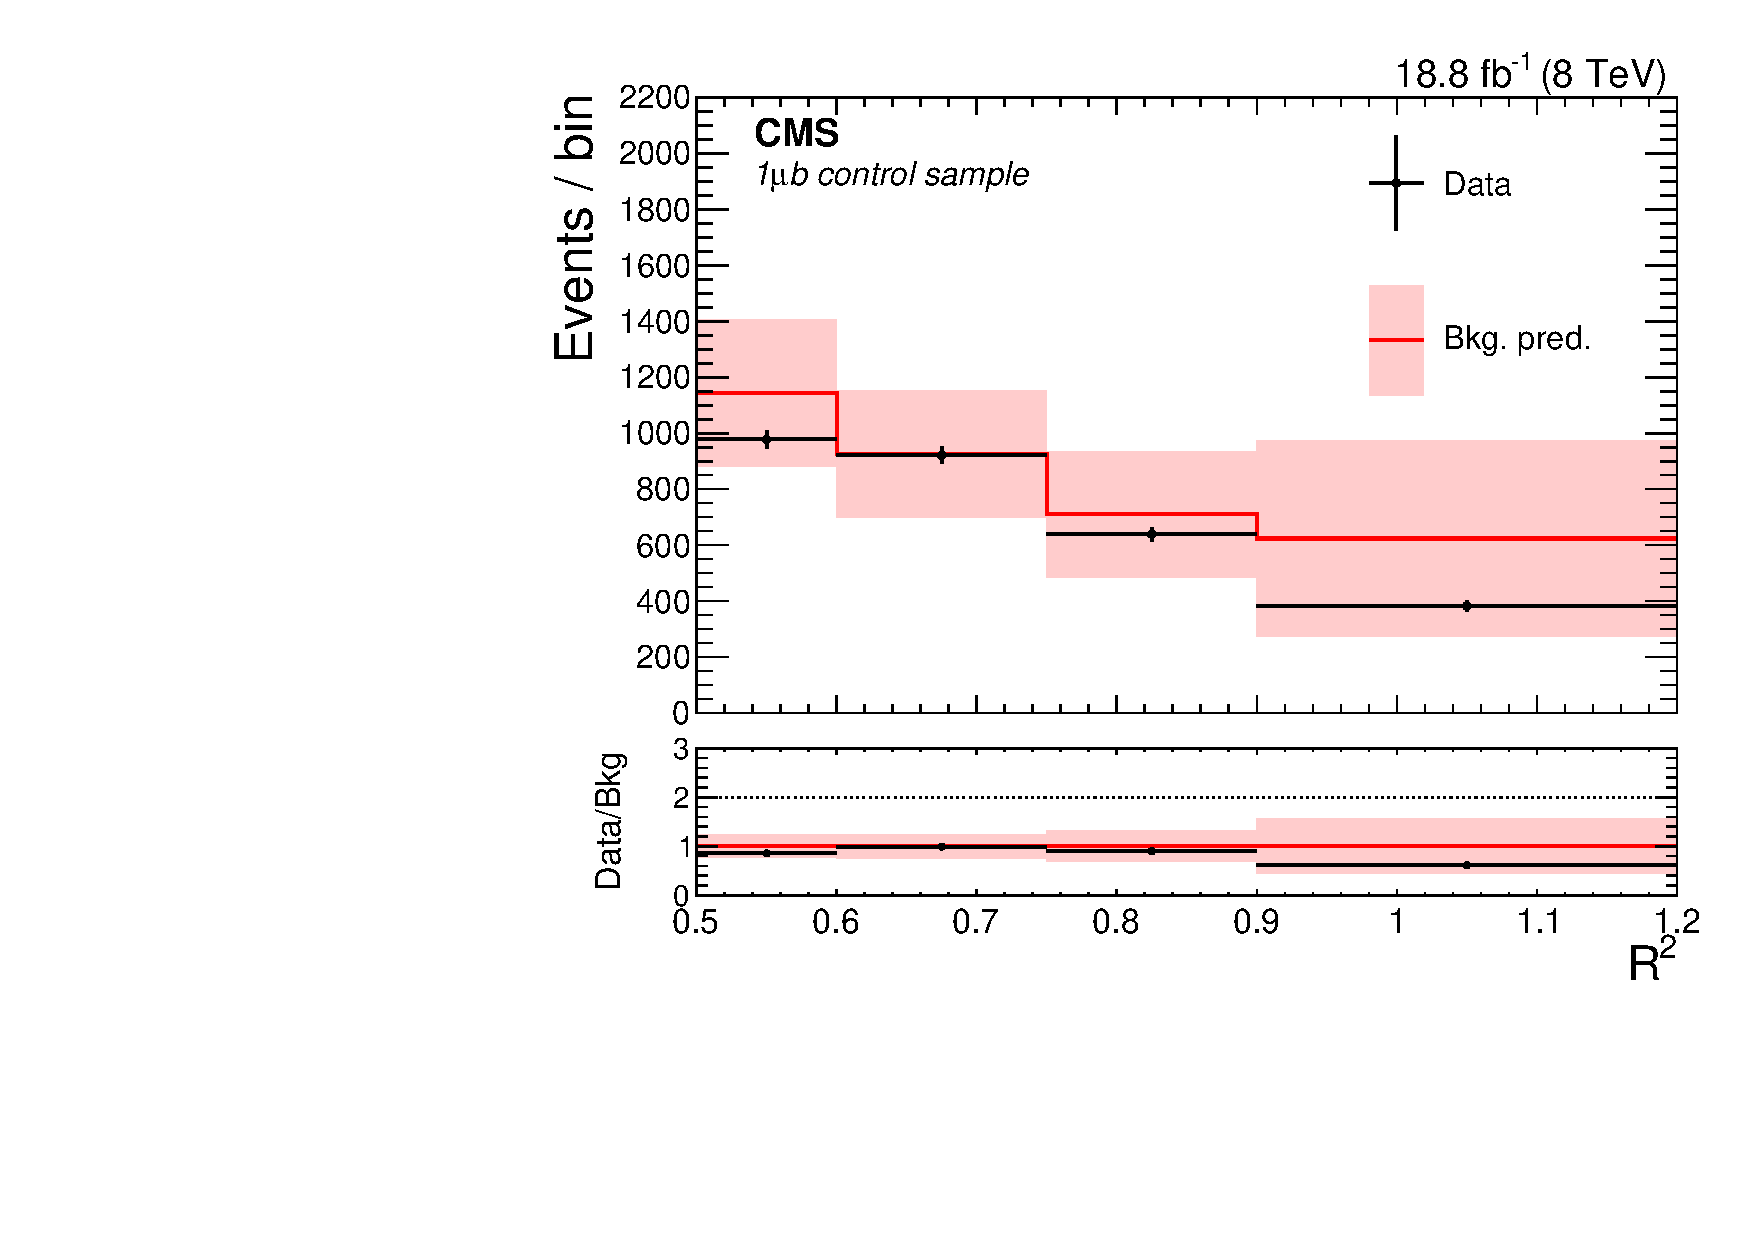
\includegraphics[width=0.5\textwidth]{DarkMatter8TeV/BtagPlots/Closure_CP_1mu1Tb_SYS_Sep.pdf} \\
 \end{tabular}
 \caption{Comparison (left ) of the observed yield and the
   prediction from simulation in the $\cPZ(\mu\mu)$b control sample
   and (right) of the observed yield in the $1\mu$b control sample and
   the background estimates from the 2$\mu$b and $\cPZ(\mu\mu)$b
   control samples, shown as a function of $\mathrm{R^2}$. The bottom
   panel of each figure shows the ratio between the data and the
   estimates. The colored band represents the statistical uncertainty
   in the left plot, and the total uncertainty in the right plot. The horizontal bars indicate 
the variable bin widths.\label{fig:Zmumub}}
\end{figure}

As a cross-check of the method, the same
procedure is applied to derive the expected yield in the 1$\mu$b
control sample (see the right plot of Fig.~\ref{fig:Zmumub}), using as input the same 2$\mu$b and $\cPZ(\mu\mu)$b
control samples. 
%The difference between this estimation and the
%observation, given in Table~\ref{tab:WITHB} and shown in
%Fig.~\ref{fig:Zmumub} (right) as a function of $\mathrm{R^2}$, is taken as
%a systematic uncertainty in the data-driven estimation in the $0\mu$b
%and $0\mu$bb samples.

The estimated background in the 0$\mu$b and 0$\mu$bb
samples is given in Table~\ref{tab:bkg0muWITHB} and shown in Fig.~\ref{fig:0muttbar}, where it is compared to
the observed yields in data. The uncertainty in the 
estimates takes into account both the statistical and systematic
components.% In the table, the yield expected from simulation is
%also quoted, computed using the NNLO production cross section. 
%The quoted uncertainty reflects the size of the simulated 
%sample.

\begin{figure}[h!]
 \centering
 \begin{tabular}{cc}
   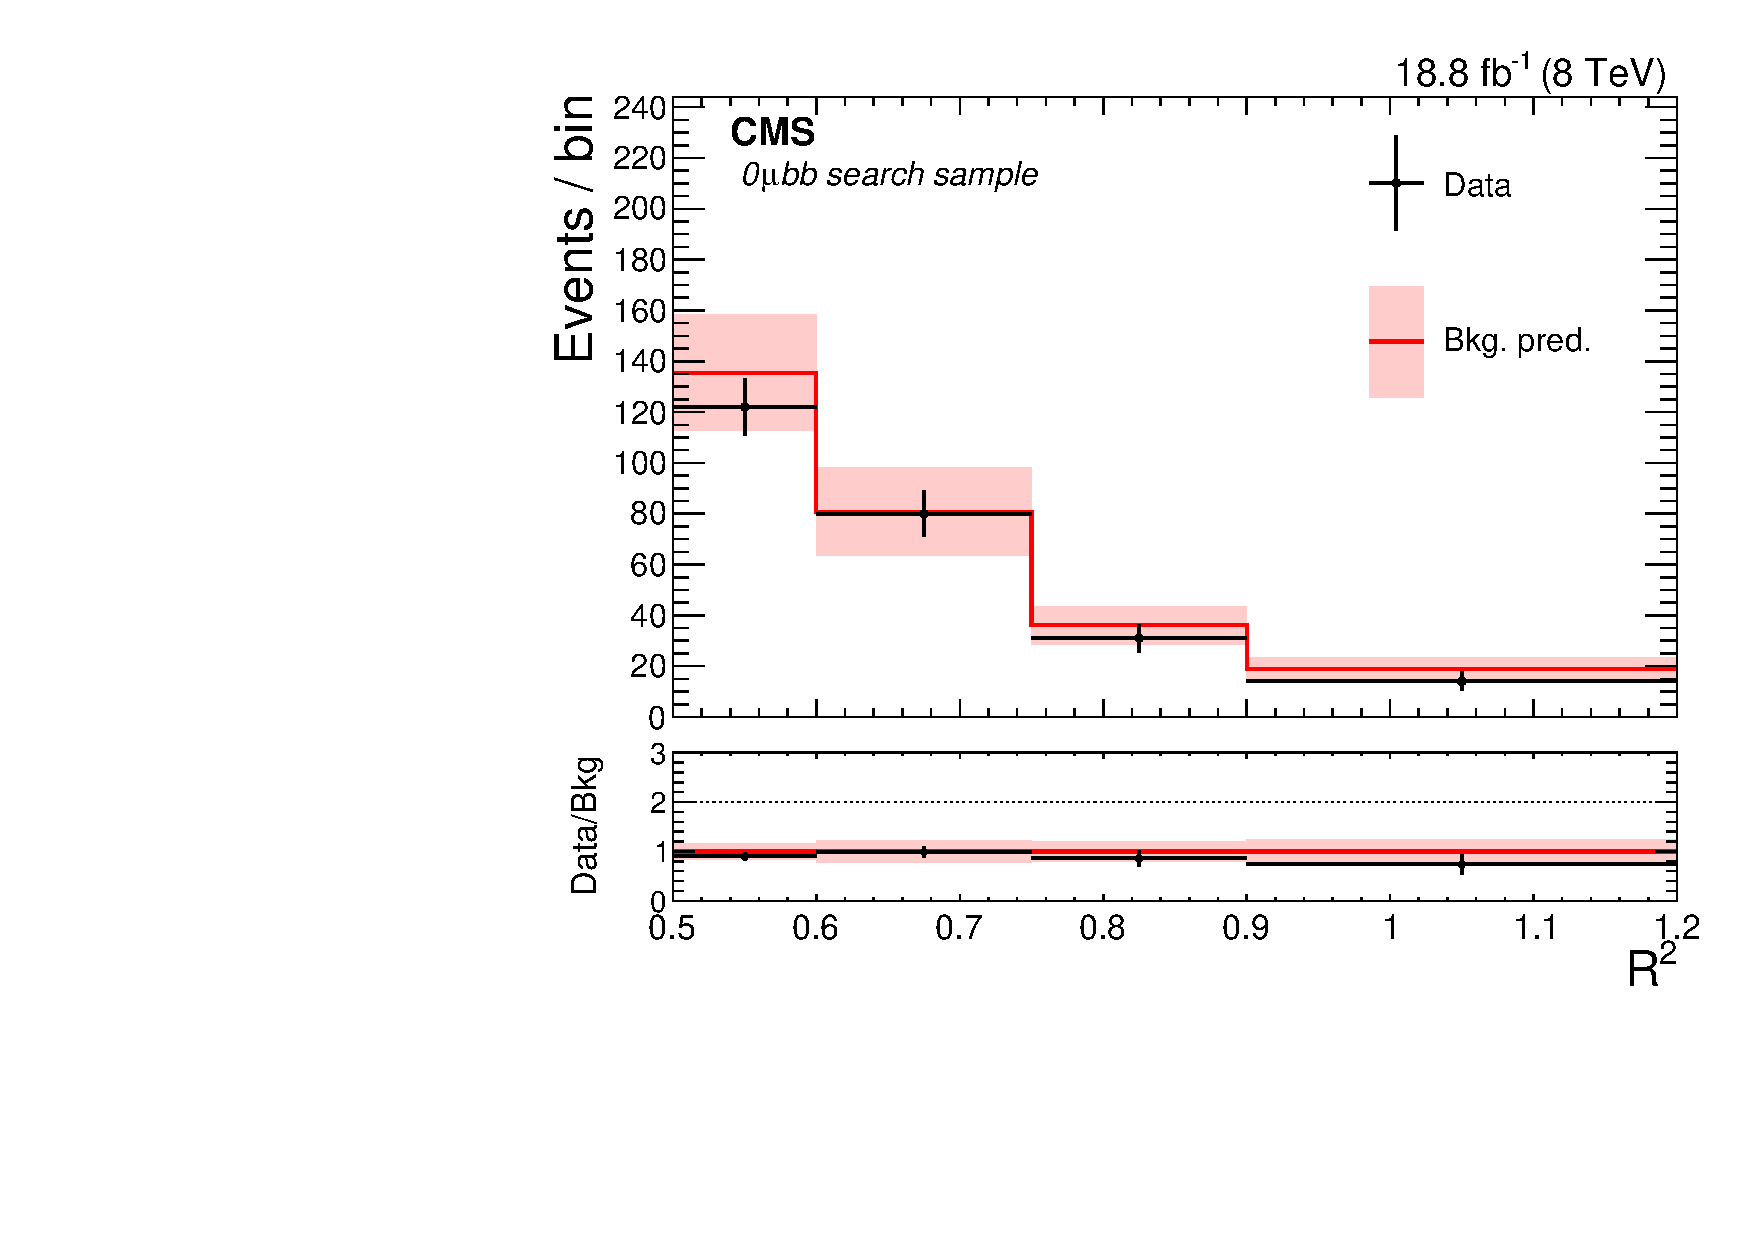
\includegraphics[width=0.5\textwidth]{DarkMatter8TeV/BtagPlots/Bkg_0mu2TbEXC_CP.pdf} & 
   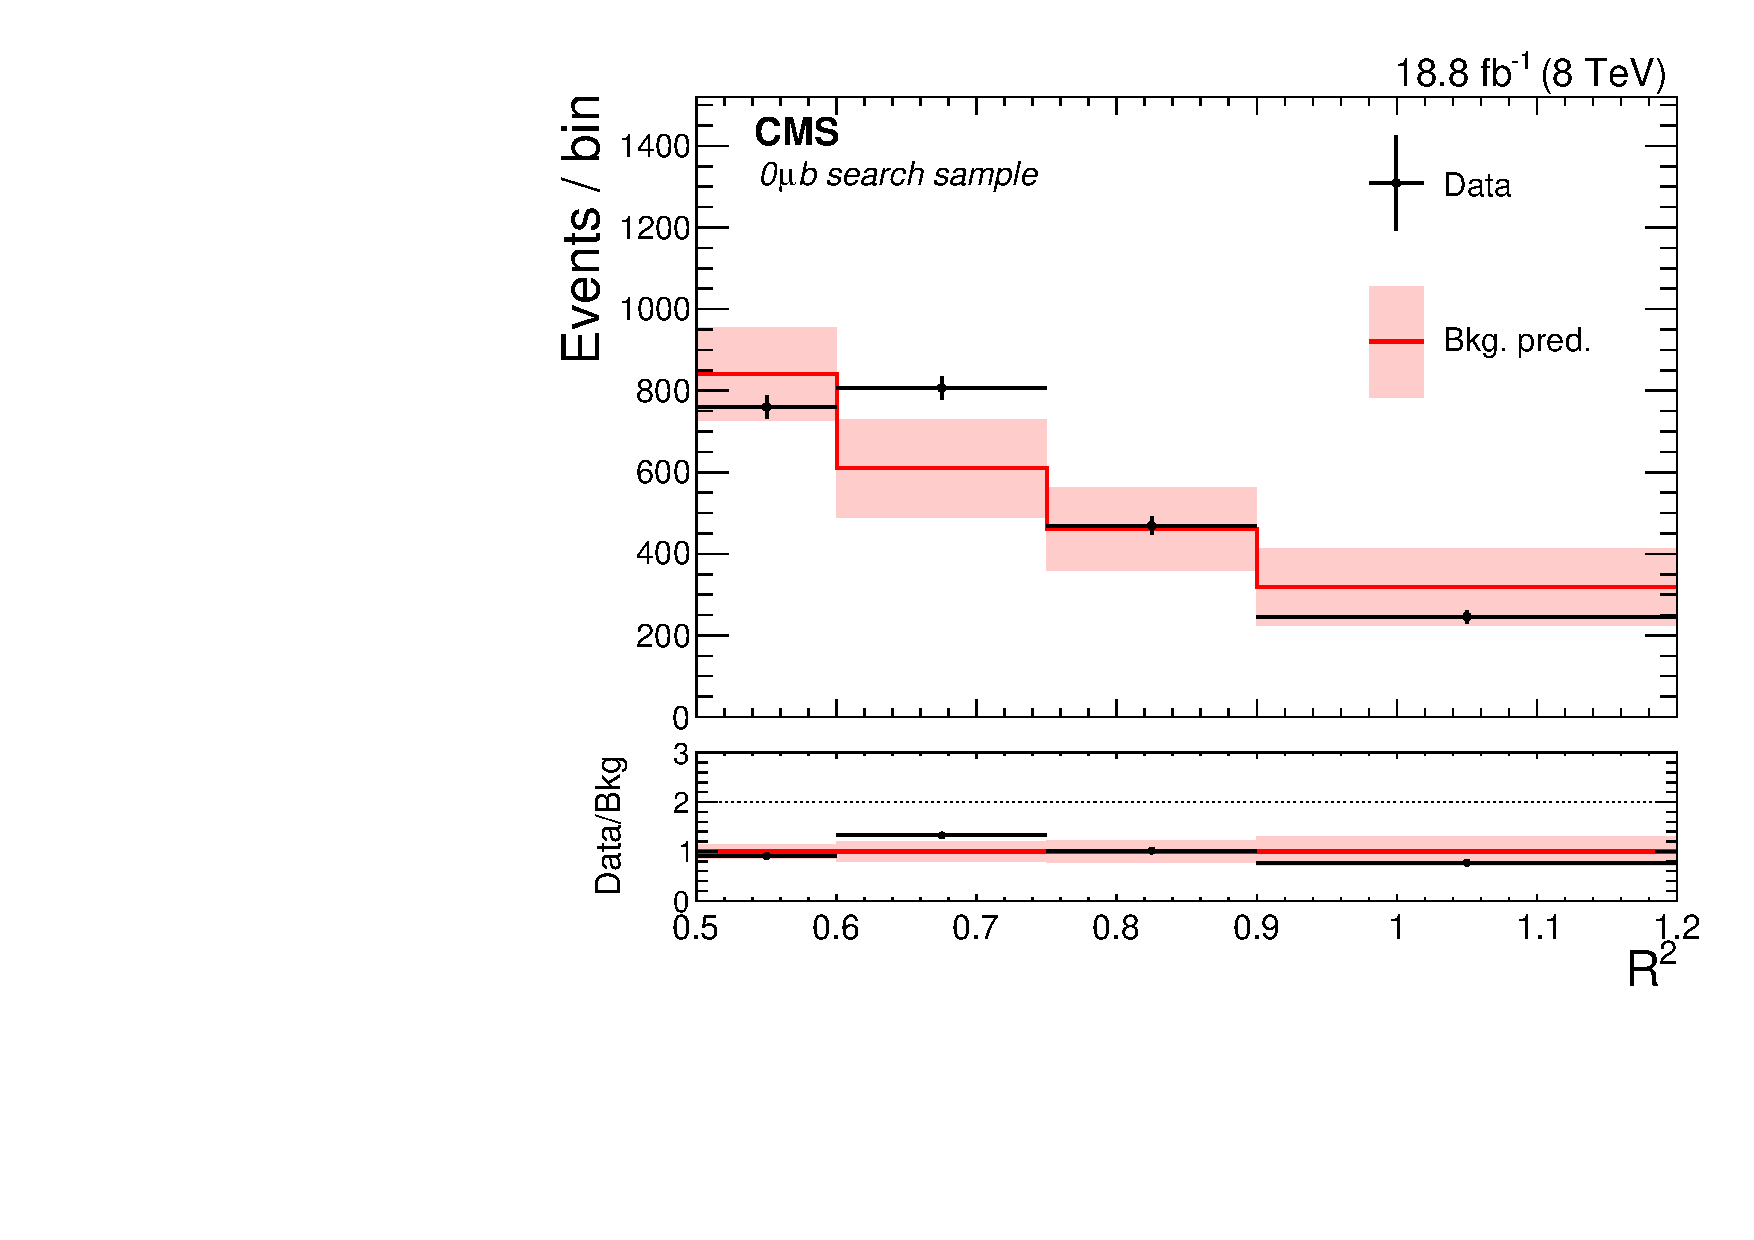
\includegraphics[width=0.5\textwidth]{DarkMatter8TeV/BtagPlots/Bkg_0mu1TbEXC_CP.pdf}\\
 \end{tabular}
 \caption{Comparison of observed event yields and background
   estimates as a function of $\mathrm{R^2}$, for the
   $0\mu$bb (left) and $0\mu$b (right) samples. The colored band
   represents the total uncertainty in the estimate. The horizontal bars indicate 
the variable bin widths.\label{fig:0muttbar}}
\end{figure}

% \begin{table}[htb]
%   \caption{ Expected background estimations
%     from simulation and observed yields for search samples
%     with b-tagged jets. A data-driven background
%     estimation is also provided, derived as described in the text.\label{tab:bkg0muWITHB}}
% \small
% \begin{tabular}{|c|c|c|c|c|c|c|c|} 
%   \hline
%   Sample  &  $\cPZ(\nu \bar \nu)$+jets  &  $\PW(\ell \nu)$+jets  &  $\cPZ(\ell \ell)$+jets  &  $\ttbar$  &  Predicted   & Predicted &  Observed \\
% &&&&& (simulation) & (data driven) & \\
% \hline
%   $0\mu$bb  &  44 $\pm$ 3  &  14 $\pm$ 2  &  0.2 $\pm$ 0.1  &  204 $\pm$ 4  &  262 $\pm$ 5  &  271 $\pm$ 37  &  247 \\ 
% \hline
%   $0\mu$b  &  417 $\pm$ 8  &  216 $\pm$ 7  &  2.4 $\pm$ 0.4  &  1480 $\pm$ 12  &  2116 $\pm$ 16  &  2231 $\pm$ 281  &  2282\\
% \hline
% \end{tabular}
% \end{table}

\begin{table}[h!]
  \caption{ Comparison of the observed yield for
    events in the search samples
    with b-tagged jets and the corresponding background
    estimates. The uncertainty in the estimates takes into account
    both the statistical and systematic components. The contribution of each individual background process is also shown, as 
estimated from simulated samples, as well as the total MC predicted yield.
\label{tab:bkg0muWITHB}}
\small
\centering
\begin{tabular}{|c|c|c|c|c|c|c|c|} 
  \hline
  Sample  &  $\cPZ(\nu \bar \nu)$+jets  &  $\PW(\ell \nu)$+jets  &
  $\cPZ(\ell \ell)$+jets  &  $\ttbar$  & MC predicted& Estimated &  Observed \\
&&&&& && \\
\hline
  $0\mu$bb  &  44 $\pm$ 3  &  14 $\pm$ 2  &  0.2 $\pm$ 0.1  &  204
  $\pm$ 4  & 262 $\pm$ 5 &  271 $\pm$ 37  &  247 \\ 
\hline
  $0\mu$b  &  417 $\pm$ 8  &  216 $\pm$ 7  &  2.4 $\pm$ 0.4  &  1480 $\pm$ 12  & 2115 $\pm$ 16 &  2230 $\pm$ 280  &  2282\\
\hline
\end{tabular}
\end{table}

\section{Systematic uncertainties}\label{sec:sys}

For each $\mathrm{R^2}$ bin in each $\mathrm{M_{\rm R}}$ category, the
difference between the observed and estimated yields in the
crosscheck analysis (see Section 6) is taken as the estimate of the uncertainty associated with the
method. The uncertainty is found to
be $\approx$ 20-40$\%$, depending on the considered bin in the
($\mathrm{M_{\rm R}}$, $\mathrm{R}^2$) plane. 

For the 0$\mu$ analysis, differences between the kinematic properties of $\PW$+jets and
$\cPZ$+jets events are additional sources of systematic uncertainty. These
differences arise from the choice of the PDF set, jet energy scale corrections, b-tagging efficiency
corrections, and trigger efficiency. These effects largely cancel
out when taking the ratio of the two processes and the resulting %resultant%
uncertainty is found to be smaller than one fifth
of the total uncertainty.  The quoted uncertainty is an upper %a conservative%
estimate of the total systematic uncertainty.
%, driven by the statistical uncertainty in the 2$\mu$ sample.

For the 0$\mu$b and 0$\mu$bb samples, both the signal and control samples are dominated by \ttbar events. The cancellation of the
systematic uncertainties is even stronger in
this case, since it does not involve different processes and different
PDFs. This systematic uncertainty is a consequence of the small size of the control sample.

Systematic uncertainties in the signal simulation
originate from the choice of the PDF set,
% the b-tagging efficiency for jets,
the jet energy scale correction, the modeling of the initial-state radiation in the event
generator, and the uncertainty in the integrated luminosity. The
luminosity uncertainty changes the signal normalization while the other
uncertainties also modify the signal shape. %This is taken into account
%through the dependence of the uncertainty size on the 
These effects are taken into account by propagating these
uncertainties into the $\mathrm{M_{\rm R}}$ category and the $\mathrm{R^2}$ bin. These uncertainties are
considered to be fully correlated across $\mathrm{M_{\rm R}}$ categories and
$\mathrm{R^2}$ bins. Typical values for the individual contributions
are given in Table~\ref{tab:sygSys}. The total uncertainty in the
signal yield is obtained by propagating the individual effects into
the $\mathrm{M_{\rm R}}$ and $\mathrm{R^2}$ variables and comparing the bin-by-bin variations with respect to the central value of the prediction
based on simulation. In the particular case of the uncertainties due
to the choice of the PDF set we have followed the PDF4LHC~\cite{Bourilkov:2006cj,Alekhin:2011sk,Botje:2011sn} prescription, using the CTEQ-6.6\cite{Nadolsky:2008zw} and MRST-2006-NNLO~\cite{Martin:2007bv} PDF sets.

\begin{table}[h!]
 \caption{\label{tab:sygSys} Systematic uncertainties associated with
  the description of the DM signal. The values indicated represent
  the typical size. The dependence of these systematic uncertainties on
  the $\mathrm{R^2}$ and $\mathrm{M_{\rm R}}$ values is taken into
  account in the determination of the results.}
 \centering
 \begin{tabular}{|c|c|} 
  \hline
  Effect  &  Uncertainty\\
  \hline
  Jet energy scale  &  3-6\%\\
  Luminosity  &  2.6\%\\
  Parton distribution functions  &  3-6\%\\
  Initial-state radiation  &  8-15\%\\
  \hline
\end{tabular}
\end{table}

\section{Results and interpretation}\label{sec:interpretation}

In Figs.~\ref{fig:0muSignalBkg1GeV}~and~\ref{fig:0muttbar} the
estimated backgrounds are compared to the observed yield in each
$\mathrm{M_{\rm R}}$ region, for events without and with
b-tagged jets, respectively. The background estimates agree with the observed
yields, within the uncertainties. This result is interpreted in terms of exclusion limits 
for several models of DM production.

%The uncertainty band associated to the estimation is
%obtained from the closure test.
%summing in quadrature the closure test uncertainty to the
%uncertainty due to the muon reconstruction efficiency. 
%The uncertainties in the parton density functions, jet energy scale
%corrections, b-tagging efficiency, and trigger efficiency are already
%accounted for by the uncertainty derived from the closure test and are
%found to be much smaller, as discussed in Section~\ref{sec:sys}. 


\subsection{Limits on dark matter production from the 0$\mu$ sample}\label{0muResults}
\label{sec:EFT0mu}
The result is interpreted in the context of a low-energy effective
field theory, in which
the production of DM particles is mediated by six and seven dimension 
operators~\cite{maverickDM,TevatronDMFrontier}. This choice allows the sensitivity of this analysis to be 
compared with the sensitivity of previous analyses~\cite{Aad:2011xw,Chatrchyan:2012me} obtaining similar 
results.

Operators of dimension six and seven are generated assuming the
existence of a heavy particle, mediating the interaction between the
DM and SM fields. To describe DM production as a local interaction, 
the propagator of the heavy mediator is expanded through an operator
product expansion. The nature of the mediator
determines the nature of the effective interaction. Two benchmark
scenarios are considered in this study, axial-vector (AV), and vector
(V) interactions~\cite{PhysRevD.85.056011}, described by the
following operators:
\begin{equation}
\label{eq:OvOva}
\hat{\mathcal{O}}_{\rm{AV}}
=
\frac{1}{\Lambda^{2}}\left(\bar{\chi}\gamma^{\mu}\gamma_{5}\chi\right)
\left(\bar{q}\gamma_{\mu}\gamma_{5}q\right) \hspace{0.05in};\hspace{0.15in}
\hat{\mathcal{O}}_{\rm{V}} =
\frac{1}{\Lambda^{2}}\left(\bar{\chi}\gamma^{\mu}\chi\right)
\left(\bar{q}\gamma_{\mu}q\right).
\end{equation}
Here  $\gamma_{\mu}$ and $\gamma_{5}$ are the Dirac matrices, $\chi$
is the DM field, and $q$ is an SM quark field. The DM particle is assumed to be a Dirac
fermion where both operators will be valid in the low-energy theory, while in the case of a Majorana DM particle the vector coupling
$\hat{\mathcal{O}}_{V}$ will vanish in the low-energy theory.
%low-energy theory
%since the vector coupling $\hat{\mathcal{O}}_{V}$ cannot appear in the
%low-energy theory for a Majorana DM particle. 
Below the cutoff energy
scale $\Lambda$, DM production is described as a contact interaction
between two quarks and two DM particles. In the case of $\math{s}$-channel
production through a heavy mediator, the energy scale $\Lambda$ is
identified with $M/\math{g_{\rm eff}}$, where $M$ is the mediator mass and 
$\math{g_{\rm eff}} = \sqrt{\math{g_{\it{q}} g_{\chi}}}$ is an effective
coupling, determined by the coupling of the mediator to quark and DM
fields, $\math{g_{\it{q}}}$ and $\math{g}_\chi$, respectively. 

%Given that the observed data yield is consistent with the standard
%model background estimation Now, we proceed to set lower limits on
%the contact interaction cutoff scale $\Lambda$. We note that the
%production cross section for this process is proportional to
%$1/\Lambda^{4}$. First we set an upper limit in the production cross 
% section and then we find lower limit for $\Lambda$ using

The results in Tables~\ref{tab:LOOKUP_VL}-\ref{tab:LOOKUP_VH} in the
Appendix are used to obtain an upper limit at 90\% confidence level
(CL) on the DM production cross section, $\sigma^{i}_{\rm{UL}}$ (where
the superscript denotes the coupling to an up or down quark). The
limits are obtained using the
LHC CLs procedure~\cite{LHC_CLS,CMS-NOTE-2011-005} and a global likelihood determined
by combining the likelihoods of the different search categories. Each
 systematic uncertainty (see Section~\ref{sec:sys}) is incorporated in the likelihood with a dedicated nuisance parameter, whose value is not known a priori but rather must be estimated from the data.

Subsequently, the cross section ($\sigma^{i}_{\rm{UL}}$) limit is translated into a lower limit $\Lambda_{\rm{LL}}$ on
the cutoff scale, through the relation:
\begin{equation}
\Lambda_{\rm LL} = \Lambda_{\rm GEN} \left(\frac{\sigma_{\rm GEN}}{\sigma_{\rm UL}}\right)^\frac{1}{4}.
\end{equation}
%where $\Lambda_{GEN} = 40$ \TeV is the cutoff scale used for the event
%generation and $\sigma_{GEN}$ is the corresponding nominal production
%cross section. 
%The fourth powers of the corresponding $\Lambda_{LL}$ values are
%summed to derive an average value for $\Lambda_{LL}$:
%%\begin{equation}
%\Lambda_{LL}^{4hroni} = (\Lambda^{u}_{LL})^4+(\Lambda^{d}_{LL})^4.
%\end{equation}
Here $\Lambda_{\rm GEN}$ and $\sigma_{\rm GEN}$ are the cutoff
energy scale and cross section of the simulated sample, respectively. 
The derived values of $\Lambda_{\rm LL}$ as a function of the DM mass,
shown in Fig.~\ref{fig:LambdaLimit}, are comparable to those derived
for the CMS monojet search~\cite{monojet8TeV}.  The analysis has been
repeated removing the events also selected by the monojet search.  The
reduction in background yields due to this additional requirement
compensates for the reduction in signal efficiency, resulting in a
negligible difference in the exclusion limit on $\Lambda$. 
%The two analysis techniques are therefore complementary.
\begin{figure}[h!]
\centering
 \begin{tabular}{cc}
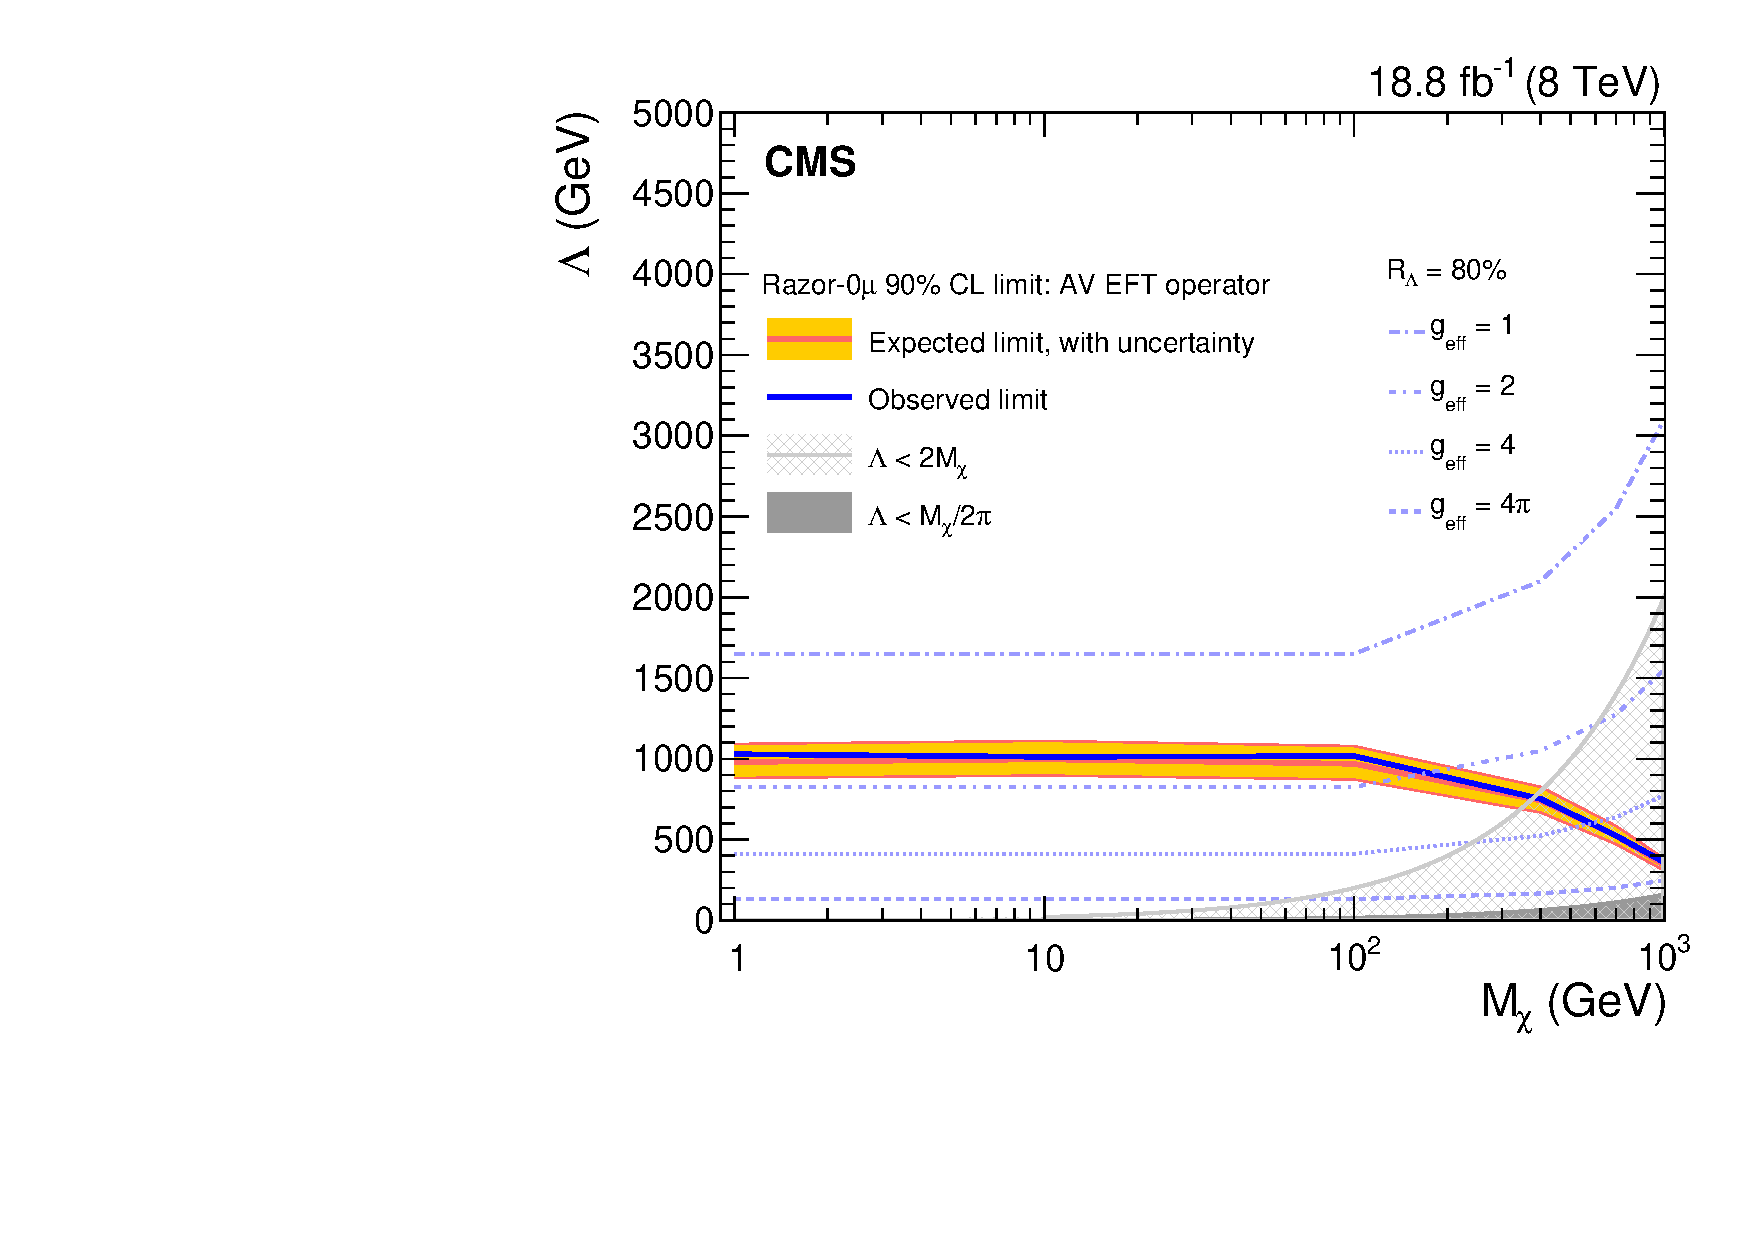
\includegraphics[width=0.5\textwidth, angle=0.]{DarkMatter8TeV/Limits/Final_av_Lambda_VarCoupling_80Percent_vNov9_2015_CWR.pdf}  & 
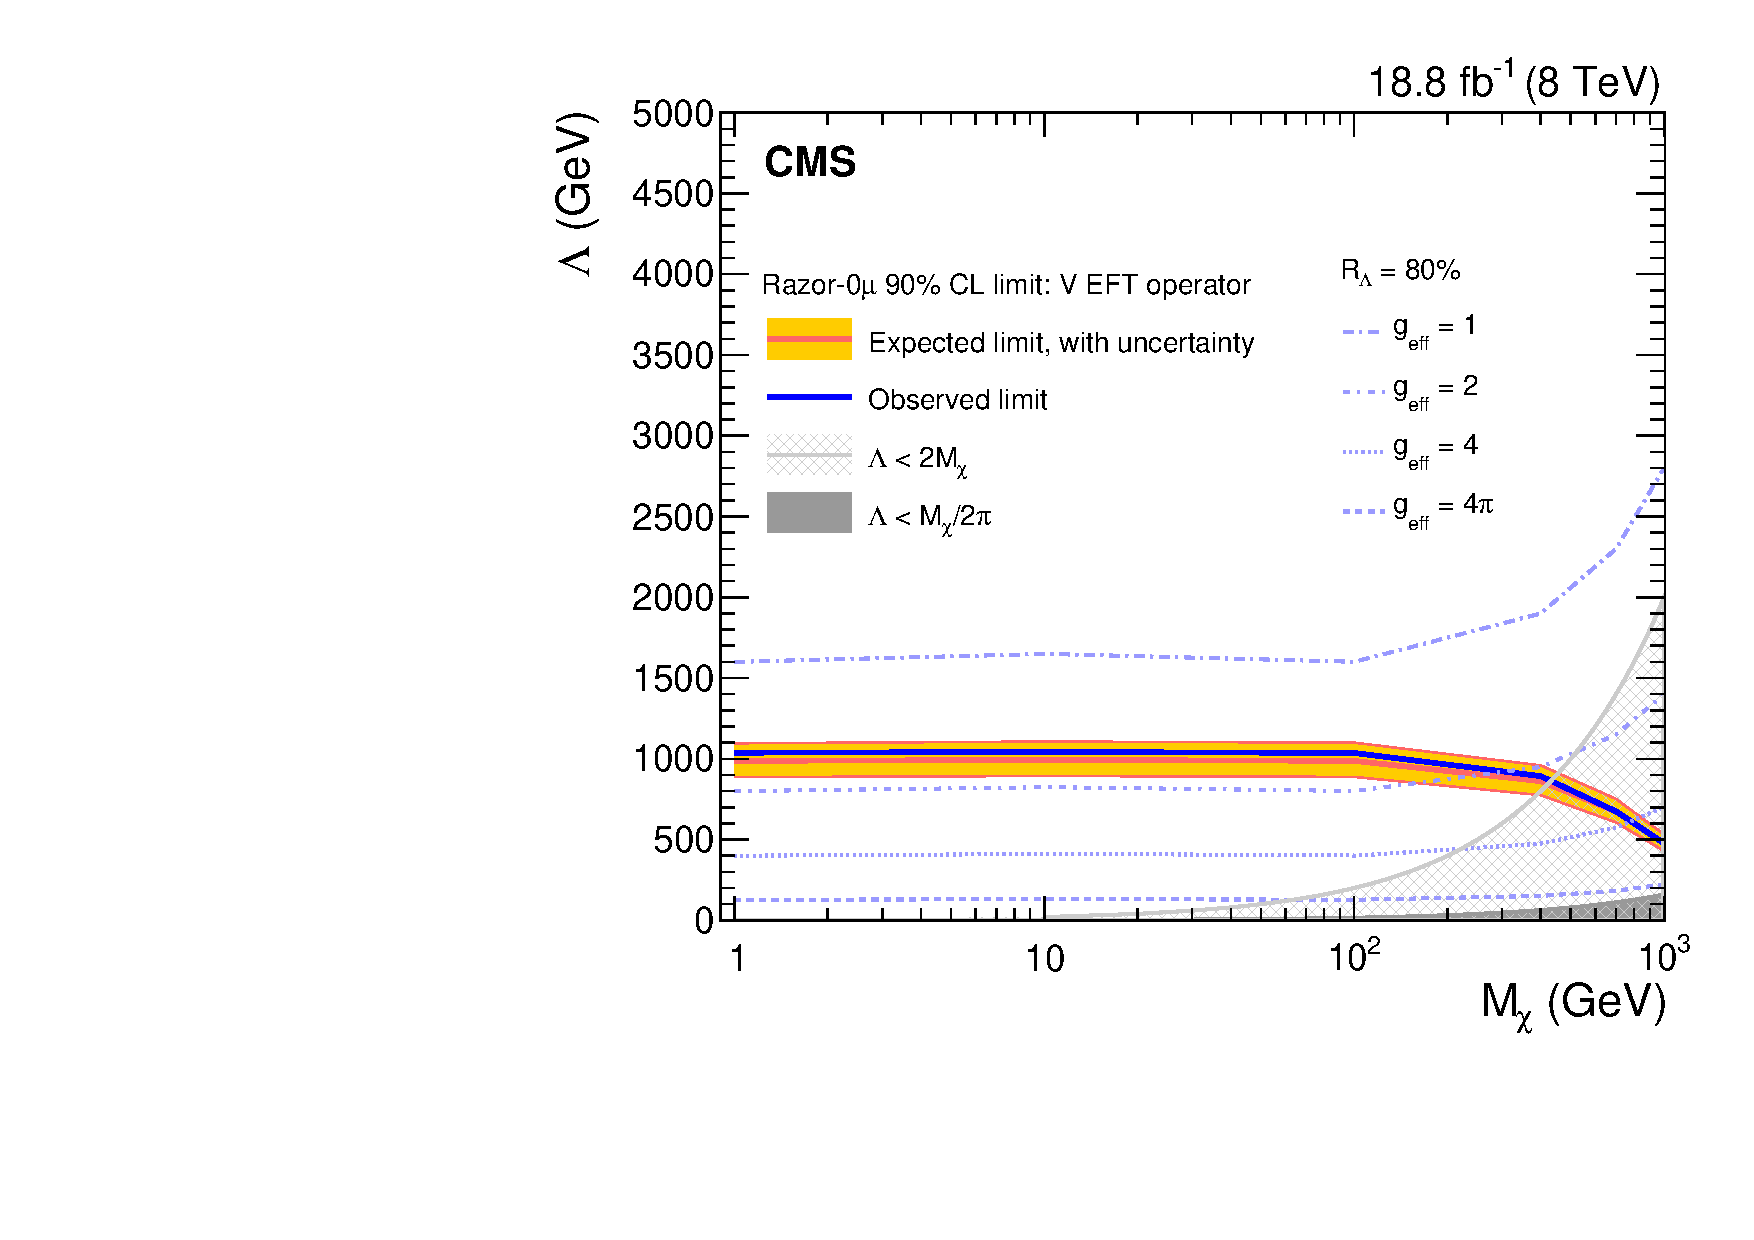
\includegraphics[width=0.5\textwidth,angle=0.]{DarkMatter8TeV/Limits/Final_v_Lambda_VarCoupling_80Percent_vNov9_2015_CWR.pdf} \\
%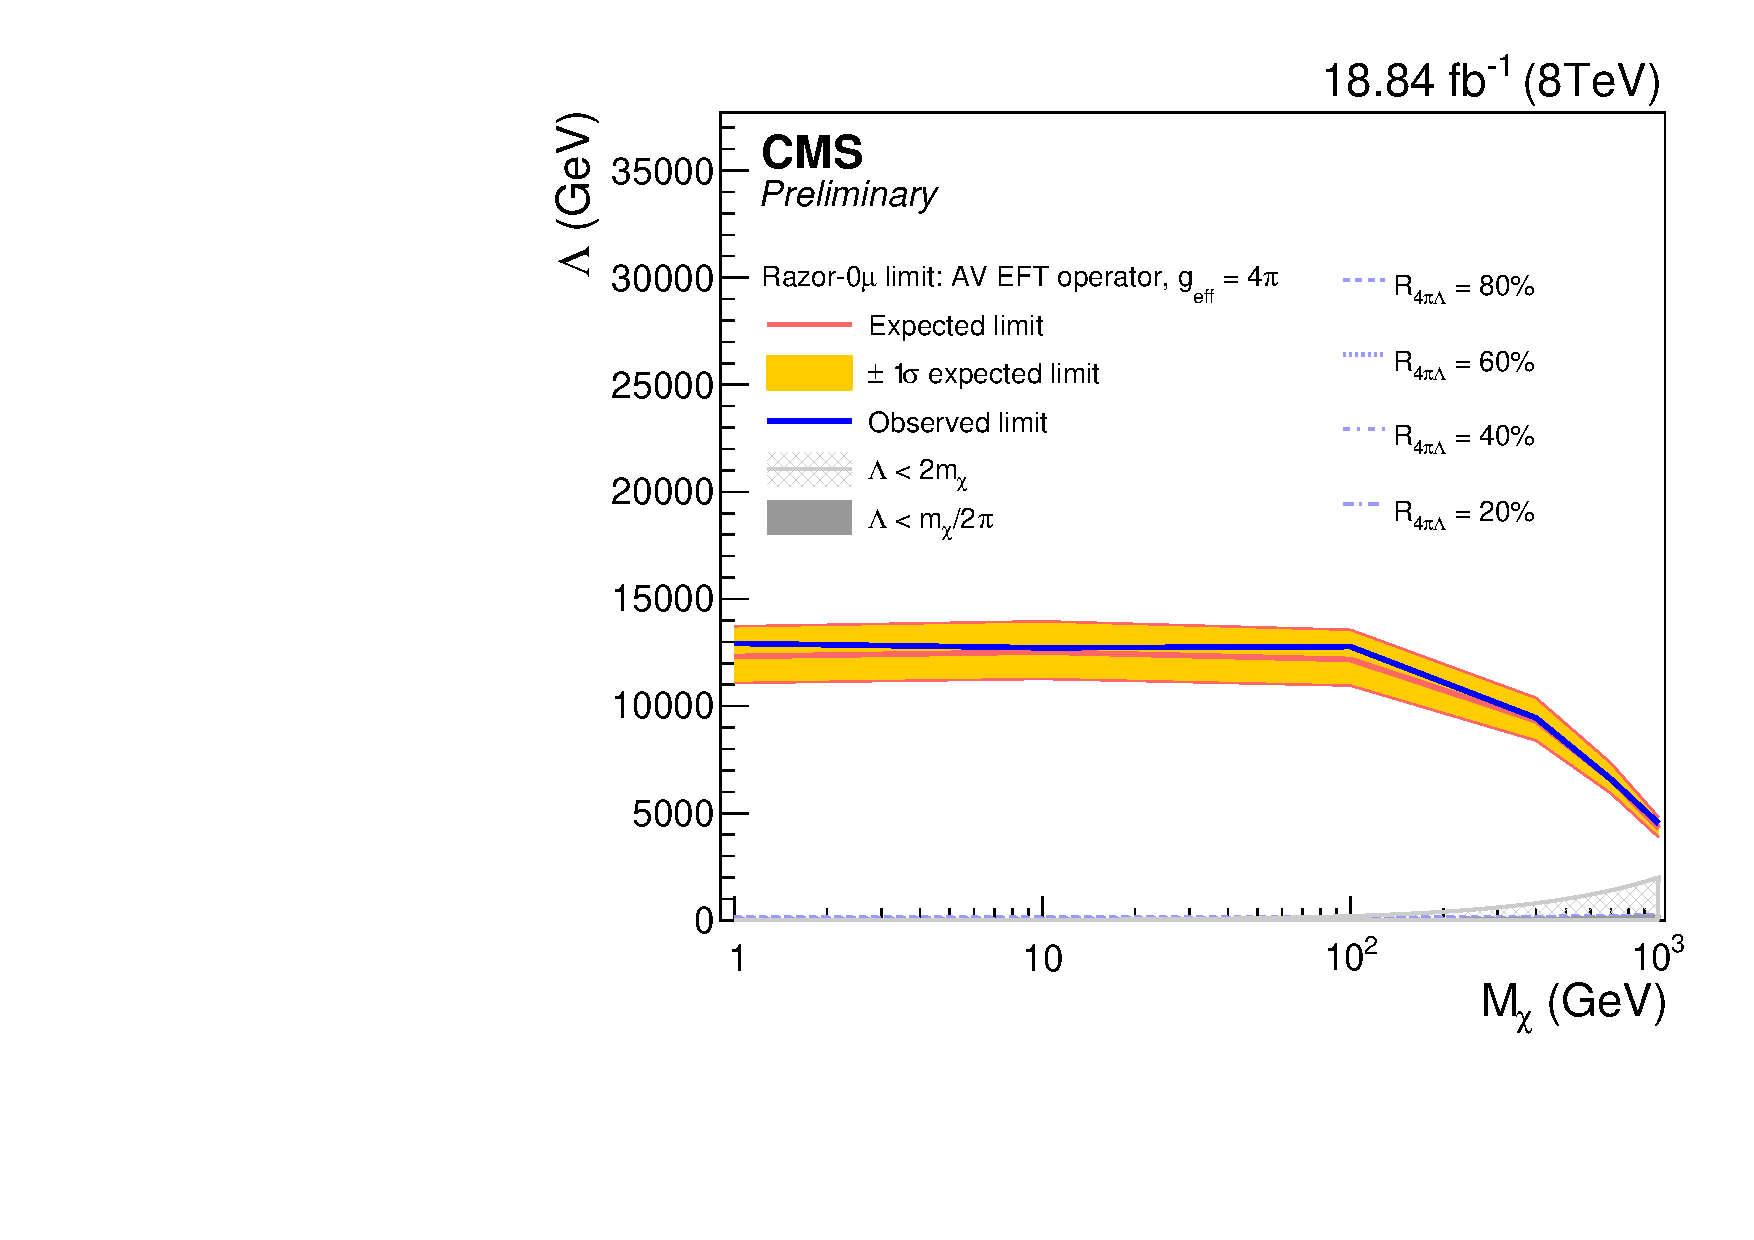
\includegraphics[width=0.5\textwidth, angle=0.]{Limits/AV_Lambda_4pi.pdf}  & 
%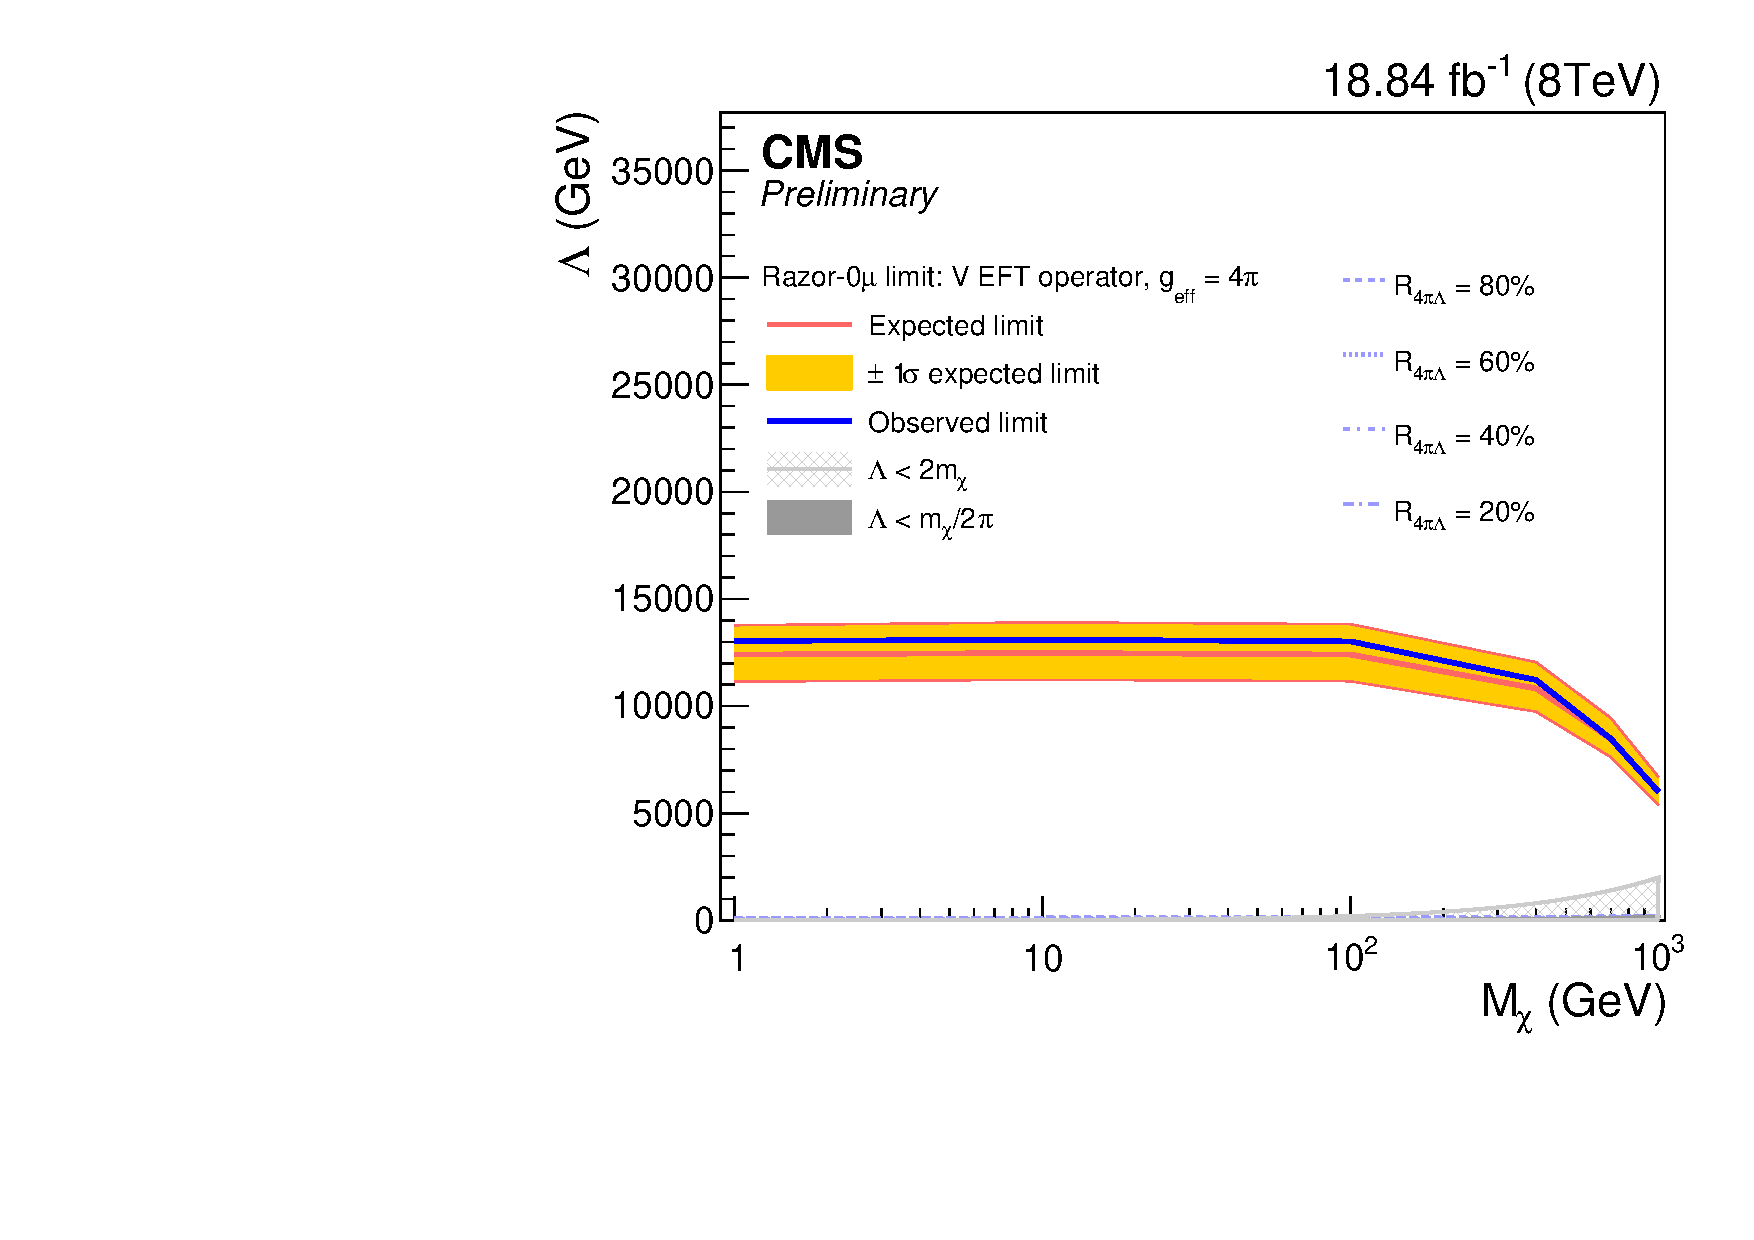
\includegraphics[width=0.5\textwidth,angle=0.]{Limits/V_Lambda_4pi.pdf} \\
%(c)  &  (d)\\
\end{tabular}
\caption{Lower limit at 90\% CL on the cutoff scale $\Lambda$ as a
  function of the DM mass $\mathrm{M}_\chi$ in the case of
  axial-vector (left) and vector (right) currents. The validity of the EFT
  is quantified by $R_\Lambda = 80\%$ contours, corresponding to
  different values of the effective coupling
  $\math{g_{\rm eff}}$.\label{fig:LambdaLimit}}
\end{figure}

The EFT framework provides a benchmark scenario to compare
the sensitivity of this analysis with that of previous searches for
similar signatures. On the other hand, the
validity of an EFT approach is limited at the LHC because a fraction 
of events under study are generated at a $\sqrt{\hat s}$ comparable to
the cutoff scale $\Lambda$~\cite{Goodman:2010ku,TevatronDMFrontier,Friedland:2011za,Buchmueller:2013dya}.  It is pointed out in the literature that for theories to be perturbative, $\math{g_{\rm eff}}$ is 
typically required to be smaller than 4$\pi$, and this condition is
unlikely to be satisfied for the entire region of phase space probed by
the collider searches. In addition, the range 
of values for the couplings being probed within the EFT may be unrealistically large. Following
the study presented in Refs.~\cite{Riotto1,Riotto2,Riotto3}, we
quantify this effect through the quantity:
\begin{equation}
R_\Lambda = \frac{\int d\mathrm{R^2} \int d \mathrm{M_{\rm R}}
  \left.\frac{d^2\sigma}{d\mathrm{R^2}  d \mathrm{M_{\rm
          R}}}\right\vert_{Q_{\rm tr}<\math{g_{\rm eff}}\Lambda} }
{\int d\mathrm{R^2} \int d \mathrm{M_{\rm R}} \frac{d^2\sigma}{d\mathrm{R^2}  d \mathrm{M_{\rm R}}} }~,
\end{equation}
where $Q_{\rm tr}$ is the momentum transferred from the mediator to the DM
particle pair. Values of $R_\Lambda$ close to unity indicate a regime in which the
assumptions of the EFT approximation hold, while a deviation from unity quantifies
the fraction of events for which the EFT approximation is still valid. We
consider the case of $\math{s}$-channel production, and we compute
$R_\Lambda$ as a function of the effective coupling $\math{g_{\rm eff}}$
in the range $0 < \math{g_{\rm eff}} \leq 4\pi$.  The contours
corresponding to $R_\Lambda = 80\%$ for different values of
$\math{g_{\rm eff}}$ are shown in Fig.~\ref{fig:LambdaLimit}. For values
of $\math{g_{\rm eff}} \gtrapprox 2$, the limit set by the analysis lies
above the $R_\Lambda = 80\%$ contour.

The exclusion limits on $\Lambda$ for the axial-vector and vector operators are transformed into upper limits on
the spin-dependent ($\sigma^{\rm SD}_{N\chi}$)~\cite{Super-Kamiokande,
  IceCube, COUPP, SIMPLE, Amole:2015lsj, Archambault:2012pm, Aprile:2013doa} and spin-independent
($\sigma^{\rm SI}_{N\chi}$)~\cite{SIMPLE, COUPP, CDMS-II, SuperCDMS, XENON100, LUX, Angloher:2014myn, Angloher:2015ewa}
DM-nucleon scattering cross section, respectively; using the following
expressions~\cite{PhysRevD.85.056011}:
\begin{eqnarray}
\sigma_{N\chi}^{\rm SD}  & = &  0.33 \frac{\mu^{2}}{\pi\Lambda_{\rm LL}^{4}}, \\
\sigma_{N\chi}^{\rm SI}  & = &  9 \frac{\mu^2}{\pi\Lambda_{\rm LL}^{4}},
\end{eqnarray}
where 
\begin{equation}
\mu = \frac{\mathrm{M}_{\chi}\mathrm{M}_{\rm
    p}}{\mathrm{M}_{\chi}+\mathrm{M}_{\rm p}}~,
\end{equation}
with $\mathrm{M}_{\rm p}$ and $\mathrm{M}_\chi$ indicating the proton and
DM masses, respectively. The numerical values of the derived limits
are given in Tables~\ref{tab:AVLimit}~and~\ref{tab:VLimit}.  The
bound on $\sigma_{N\chi}$ as a function of $\mathrm{M}_\chi$ is shown
in Fig.~\ref{fig:DMNxsec} for spin-dependent and spin-independent DM-nucleon scattering.

In order to compare our results with those from direct detection experiments, the experimental bounds in~\cite{SIMPLE, COUPP,CDMS-II,
  SuperCDMS, XENON100, LUX,Super-Kamiokande, IceCube, COUPP, SIMPLE}
are translated into bounds on $\Lambda$. This comparison is shown in
Fig.~\ref{fig:LambdaComplete}. This translation is well
defined since the momentum transfer in most direct detection
experiments is low compared to the values of $\Lambda$ being probed,
and thus the EFT approximations in question are mostly valid.
\begin{table}[h!]        
\begin{center}
\caption{\label{tab:AVLimit}% Limit results for axial-vector current
  %dark matter production.
The 90\% CL limits on DM production in the case of axial-vector
couplings. Here, $\sigma^{u}_{\rm UL}$ and $\sigma^{d}_{\rm UL}$ are
the observed upper limits on the production cross
section for u and d quarks, respectively; $\Lambda_{\rm LL}$
is the observed cutoff energy scale lower limit; and $\sigma_{N\chi}$
is the observed DM-nucleon scattering cross section upper limit.}
\begin{tabular}{|c|c|c|c|c|}       
\hline
$\mathrm{M}_\chi$  (GeV) &  $\sigma^{u}_{\rm UL}$(pb)  &  $\sigma^{d}_{\rm UL}$(pb)
  &  $\Lambda_{\rm LL}$ (\GeV)  &  $\sigma_{N\chi}$  $(\cm^{2})$ \\
\hline
1  & 0.39  &  0.45  &  1029 & $8.5\times 10^{-42}$ \\
10  &  0.43  &  0.45   & 1012 & $2.9\times 10^{-41}$\\
100  &  0.30  & 0.37  &  1017 & $3.3\times 10 ^{-41}$\\
400  & 0.25  &  0.26  &  752 & $1.1\times 10^{-40}$\\
700  &  0.21  &  0.26  &  524 & $4.7\times 10^{-40}$\\
1000  & 0.17  & 0.22  &  360 & $2.1\times 10^{-39}$\\
\hline
\end{tabular}
\end{center}
\end{table}
\begin{table}[h!]        
\caption{\label{tab:VLimit}% Limit results for vector current dark
  %matter production. Limits are quoted at 90\% CL.
%The 90\% CL upper limits for DM production with vector couplings.
The 90\% CL limits on DM production in the case of vector
couplings. Here, $\sigma^{u}_{\rm UL}$ and $\sigma^{d}_{\rm UL}$ are
the observed upper limits on the production cross
section for u and d quarks, respectively; $\Lambda_{\rm LL}$
is the observed cutoff energy scale lower limit; and $\sigma_{N\chi}$
is the observed DM-nucleon scattering cross section upper limit.}
\begin{center}
\begin{tabular}{|c|c|c|c|c|}       
\hline
$\mathrm{M}_\chi$  (GeV) &  $\sigma^{u}_{\rm UL}$(pb)  &  $\sigma^{d}_{\rm UL}$(pb)
  &  $\Lambda_{\rm LL}$ (\GeV)  &  $\sigma_{N\chi}$  $(\cm^{2})$\\
\hline
1  &  0.41  &   0.38  & 1038 & $2.3\times 10^{-40}$ \\
10  &  0.36  &  0.45  & 1043 & $6.9\times 10^{-40}$\\
100  &  0.33  &   0.44 & 1036 & $8.3\times 10 ^{-40}$\\
400  &  0.23  &  0.35  & 893 & $1.5\times 10^{-39}$\\
700  &  0.22  &  0.27  & 674 & $4.7\times 10^{-39}$\\
1000  &  0.22  &  0.27  & 477 & $1.8\times 10^{-38}$\\
\hline
\end{tabular}
\end{center}
\end{table}
\begin{figure}[h!]
\centering
 \begin{tabular}{cc}
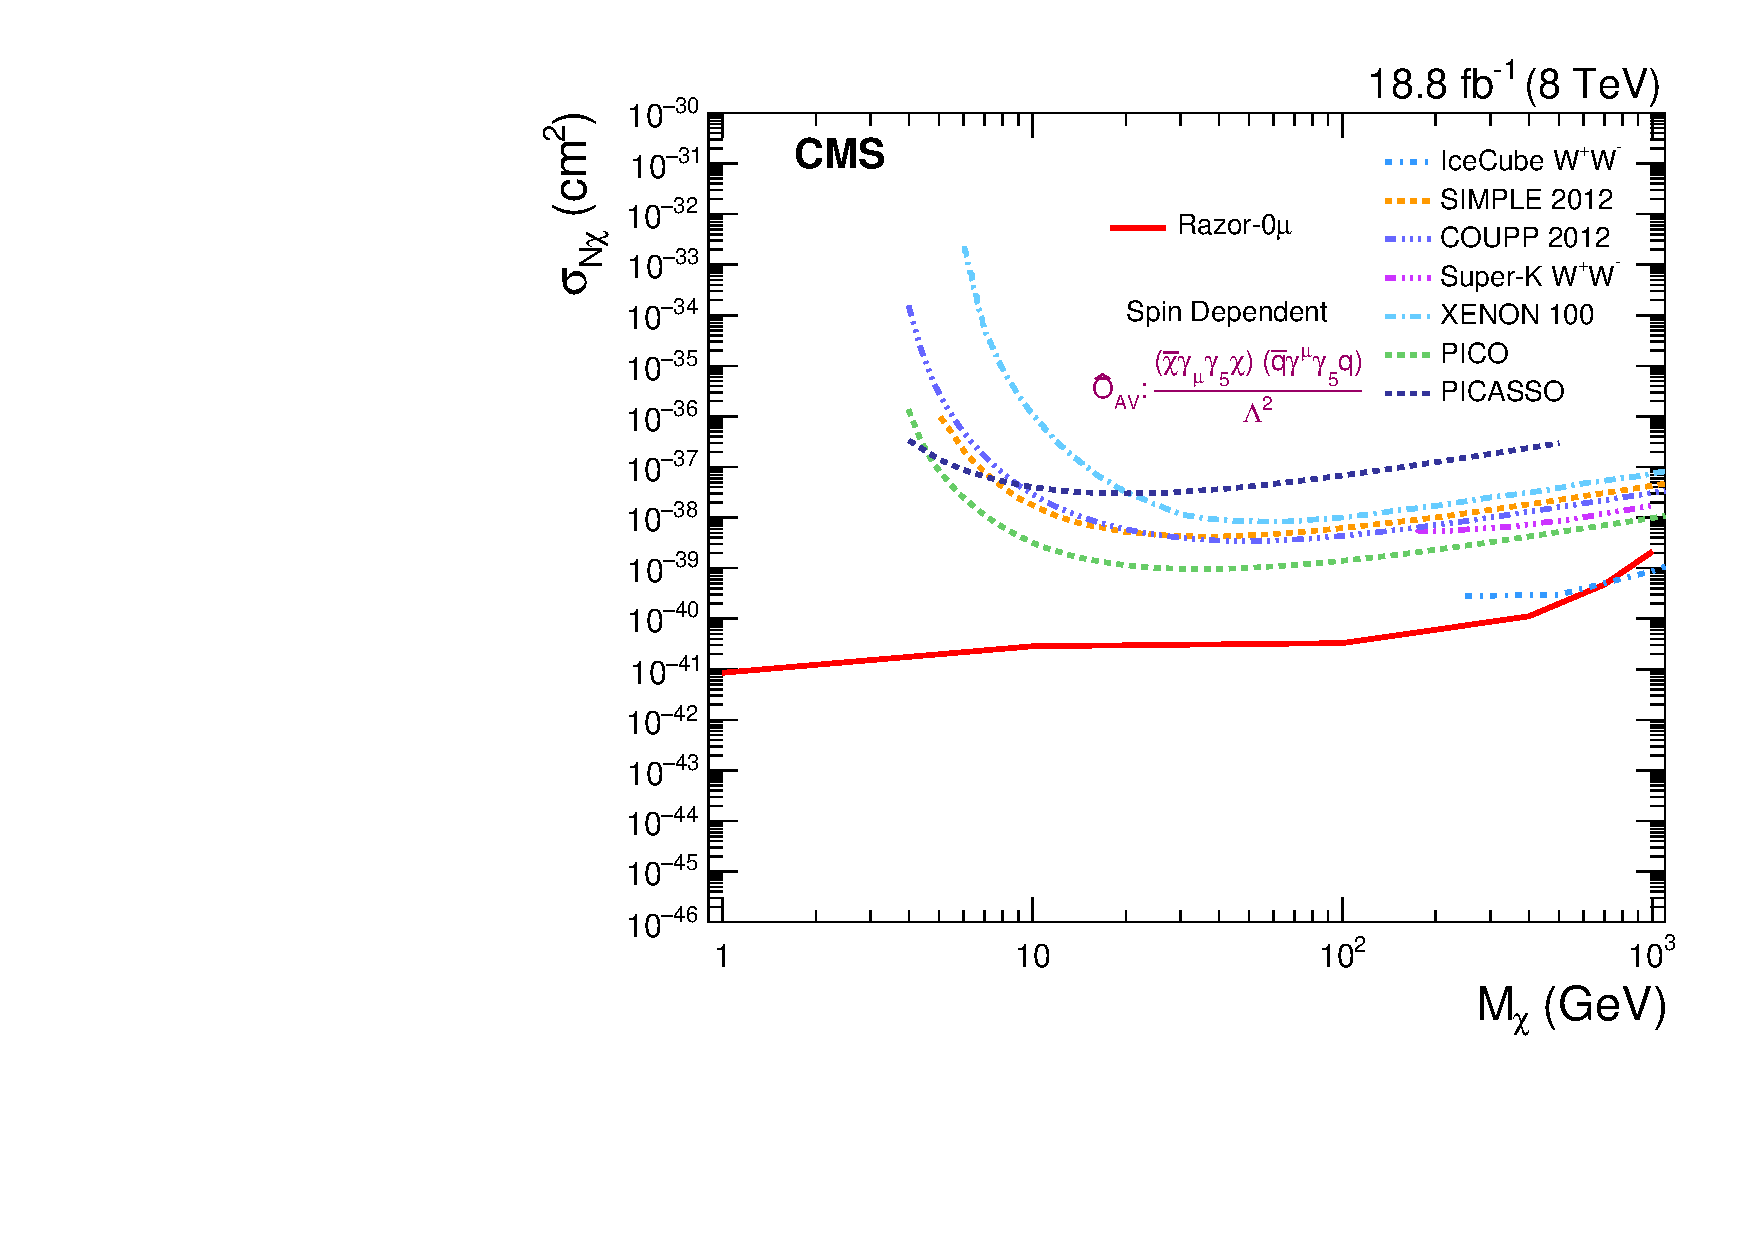
\includegraphics[width=0.5\textwidth, angle=0.]{DarkMatter8TeV/Limits/SD_TOYS_FINAL_Nov9_CWR_RazorOnly.pdf}  & 
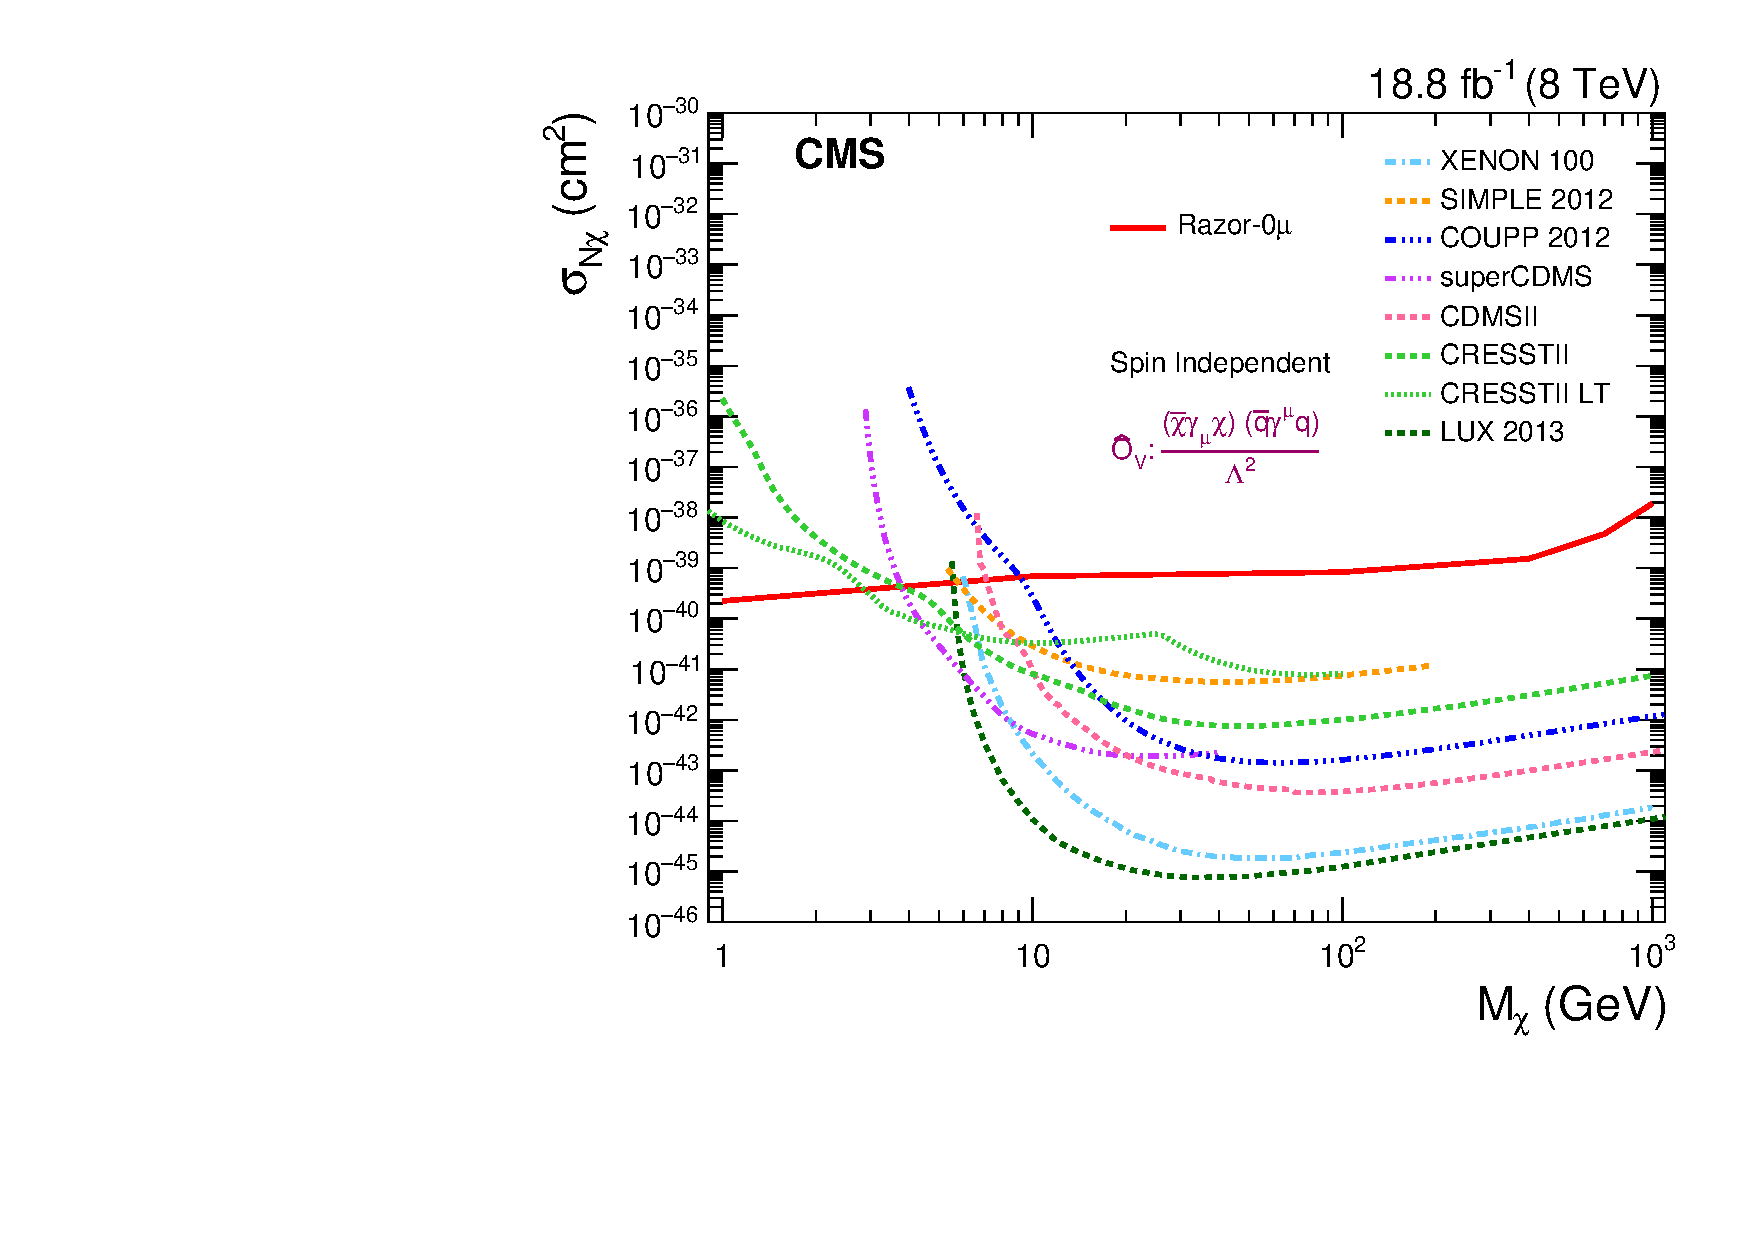
\includegraphics[width=0.5\textwidth,angle=0.]{DarkMatter8TeV/Limits/SI_TOYS_FINAL_Nov9_CWR_RazorOnly.pdf}\\
\end{tabular}
\caption{Upper limit at 90\% CL on the DM-nucleon scattering cross
  section $\sigma_{N\chi}$ as a function of the DM mass
  $\mathrm{M}_\chi$ in the case of spin-dependent axial-vector (left)
  and spin-independent vector (right) currents. A selection of
  representative direct detection experimental bounds are also shown.\label{fig:DMNxsec}}
\end{figure}
\begin{figure}[h!]
\centering
 \begin{tabular}{cc}
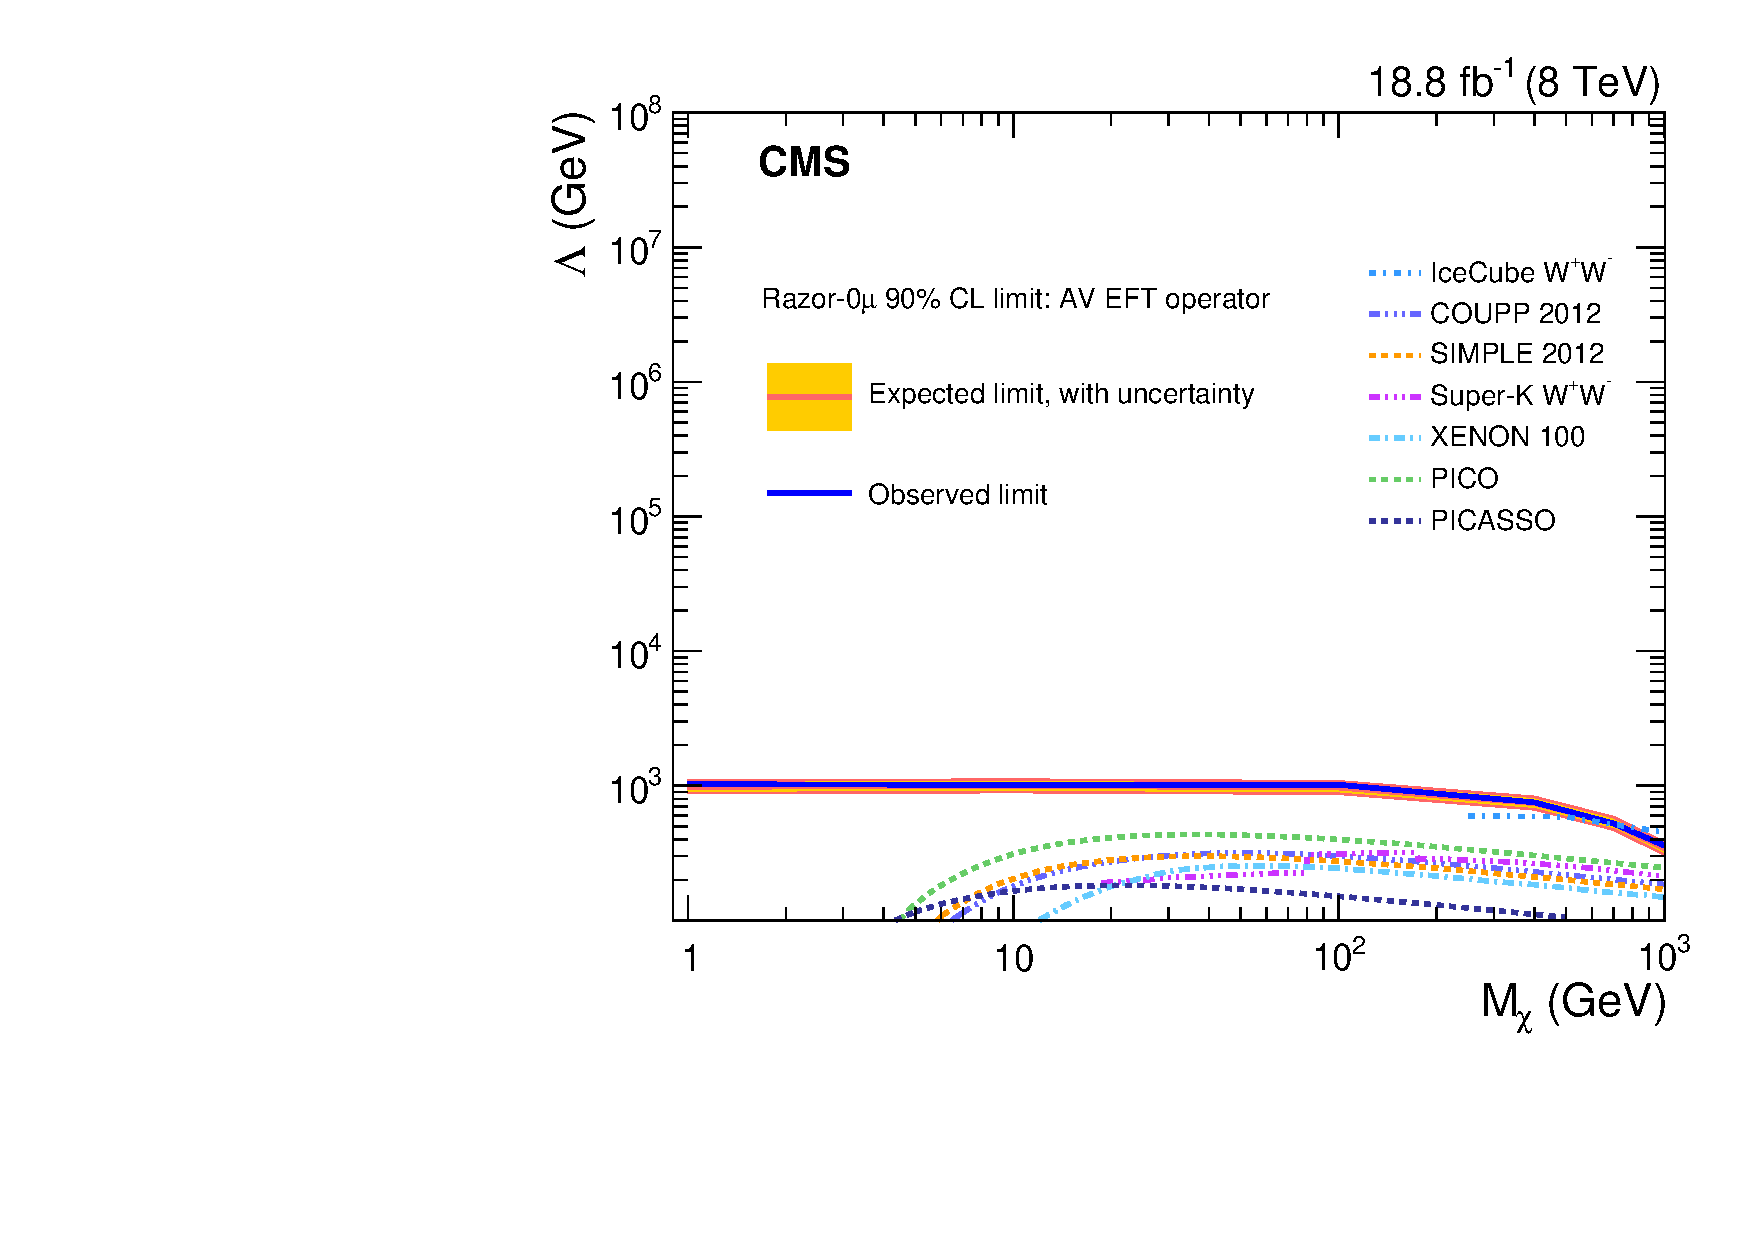
\includegraphics[width=0.5\textwidth, angle=0.]{DarkMatter8TeV/Limits/Final_AV_Lambda_WithDD_vNov9_2015_CWR.pdf}  & 
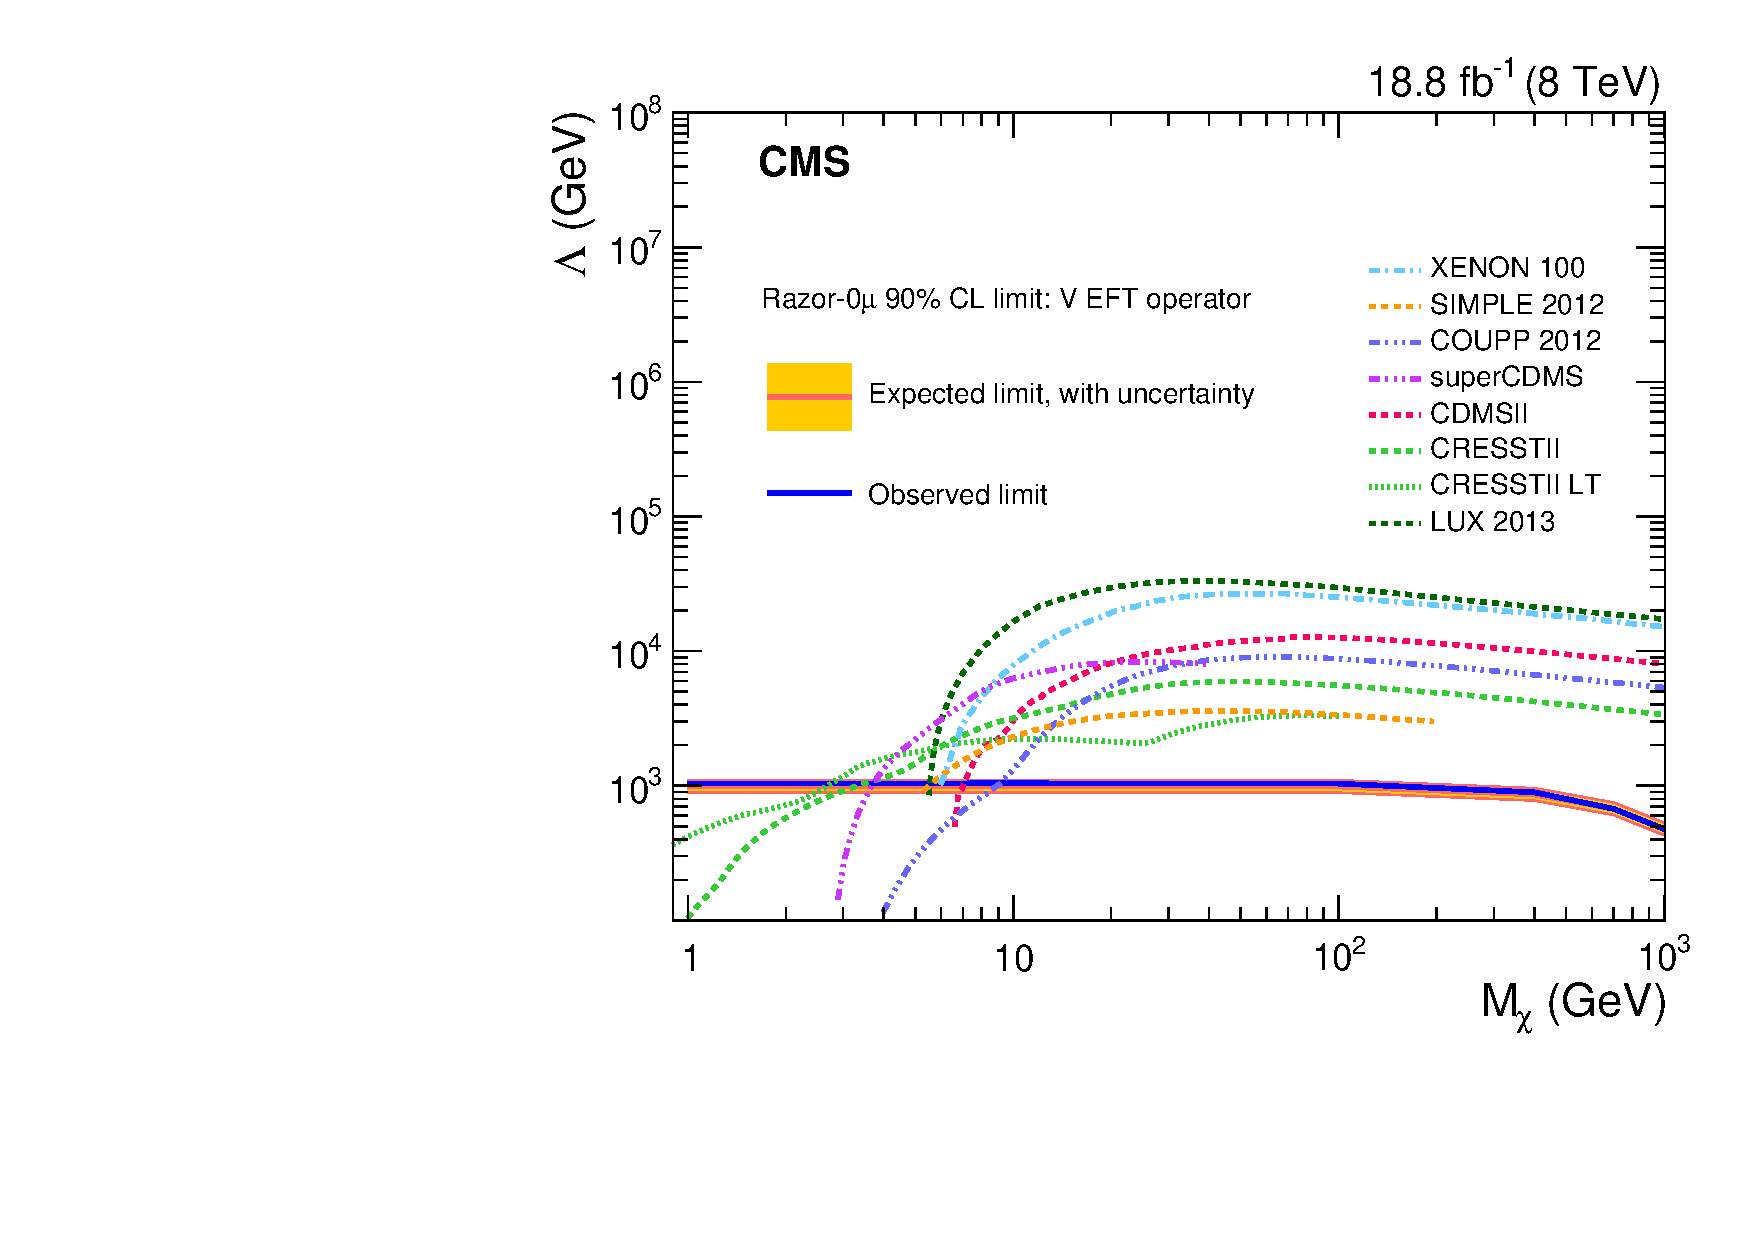
\includegraphics[width=0.5\textwidth,angle=0.]{DarkMatter8TeV/Limits/Final_V_Lambda_WithDD_vNov9_2015_CWR.pdf}\\
\end{tabular}
\caption{Lower limit at 90\% CL on the cutoff scale $\Lambda$ as a
  function of the DM mass $\mathrm{M}_\chi$ in the case of
  axial-vector (left) and vector (right) currents. A selection of direct detection
  experimental bounds are also shown.\label{fig:LambdaComplete}}
\end{figure}
\subsection{Limits on dark matter production from the 0$\mu$b and 0$\mu$bb samples}

The results from the 0$\mu$b and 0$\mu$bb samples are interpreted in
an EFT scenario, following a methodology similar to that of
Section~\ref{sec:EFT0mu}. In this case, a heavy scalar mediator
 is considered~\cite{Lin:2013sca}, generating an operator:
\begin{equation}
\label{eq:Os}
\hat{\mathcal{O}}_{S} = \frac{\mathrm{M}_{q}}{\Lambda^{3}}\bar{\chi}\chi \bar{q}q.
\end{equation}

The dependence on the mass, induced by the scalar nature of the
mediator, implies a stronger coupling to third-generation quarks,
enhancing the sensitivity of the 0$\mu$b and 0$\mu$bb samples to this
scenario. Unlike the case of V and AV operators, the production cross
section for this process is proportional to $1/\Lambda^{6}$. The
value of $\Lambda_{\rm LL}$ is then derived as
\begin{equation}
\Lambda_{\rm LL} = \Lambda_{\rm GEN} \left(\frac{\sigma_{\rm
      GEN}}{\sigma_{\rm UL}}\right)^{\frac{1}{6}}.
\end{equation}

%Here $\Lambda_{\rm GEN}$ and $\sigma_{\rm GEN}$ are the cut-off
%energy scale and cross section of the simulated sample, respectively.

Given the results of Table~\ref{tab:bkg0muWITHB} we proceed to set limits at 90\%
CL on the cutoff scale (see Table~\ref{tab:MonobLimit}) using the LHC
CLs procedure already presented. To quantify the validity of the EFT we follow the
discussion in Section~\ref{sec:EFT0mu}, considering an interaction
mediated by an $\math{s}$-channel produced particle. The operator of
Eq.~(\ref{eq:Os}) is suppressed by an additional factor
$m_\mathrm{b}$/$\Lambda$ with respect to the operators in
Eq.~(\ref{eq:OvOva}). As a result, for a given value of the coupling
$\math{g_{\rm eff}}$, smaller values of $\Lambda$ are probed in this
case. The observed limit stays below the contours derived for
$R_{\Lambda} = 80\%$, even when the coupling is fixed to the largest
value considered, $\math{g_{\rm eff}} = 4\pi$, as shown in the left plot
of Fig.~\ref{fig:LimitLambdab}. For the same choice of coupling,
the derived limit on $\Lambda$ would correspond to $R_{\Lambda}
\approx 25\%$, as shown in the right plot of
Fig.~\ref{fig:LimitLambdab}. Only for $\math{g}_{\rm eff} > 4\pi$ does the
observed limit correspond to values of $R_{\Lambda}>80\%$. This
requirement implies a UV completion of the EFT beyond
the perturbative regime. For this reason, this result is not
interpreted in terms of an exclusion limit on $\sigma_{N\chi}$.

% \begin{table}[!h]
% \begin{center}
% \caption{\label{tab:MonobLimit} Limit results for scalar current dark
%   matter production. Limits are quoted at 90\% CL. $\sigma^{\rm
%     obs}_{\rm UL}$ is the observed upper limit on the production cross
% section, $\Lambda^{\rm obs}_{\rm LL}$ and $\Lambda^{\rm exp}_{\rm LL}$
% are the observed and expected cut-off energy scale lower limit, respectively.}
% \begin{tabular}{|c|c|c|c|c|}
% \hline
%$\mathrm{M}_\chi$  (GeV) & $\sigma^{\rm obs}_{\rm UL}$(pb) & $\Lambda^{\rm obs}_{\rm LL}$
%                                              (GeV) & $\Lambda^{\rm exp}_{\rm LL}$ (GeV)  &  $\sigma_{N\chi}$  $(\cm^{2})$\\
% \hline
% 0.1  &  5.4   &  43.0  &  48.2  &  $2.3\times 10^{-39}$ \\
% 1  &  3.8   &  45.3  &  49.9  &  $1.7\times 10^{-39}$ \\
% 10  &  6.3   &  43.2  &  48.4  &  $2.2\times 10^{-39}$\\
% 100  &  0.8  &  53.7  &  55.1  &  $0.6\times 10 ^{-39}$\\
% 200  &  0.7  &  47.2  &  48.3  &  $1.3\times 10^{-39}$\\
% 300  &  2.8  &   32.5  &  35.8  &  $1.2\times 10^{-38}$\\
% 400  &  2.8  &  28.3  &  30.8  &  $2.8\times 10^{-38}$\\
% 1000  &  1.7  &  13.2  &  13.8  & $2.7\times 10^{-36}$\\
% \hline
% \end{tabular}
% \end{center}
% \end{table}

\begin{table}[!h]
\begin{center}
\caption{\label{tab:MonobLimit} The 90\% CL limits on DM production in
  the case of scalar couplings. Here, $\sigma^{\rm
    obs}_{\rm UL}$ is the observed upper limit on the production cross
section, $\Lambda^{\rm obs}_{\rm LL}$ and $\Lambda^{\rm exp}_{\rm LL}$
are the observed and expected cutoff energy scale lower limit, respectively.}
\begin{tabular}{|c|c|c|c|}
\hline
$\mathrm{M}_\chi$  (GeV) & $\sigma^{\rm obs}_{\rm UL}$(pb) & $\Lambda^{\rm obs}_{\rm LL}$
                                             (GeV) & $\Lambda^{\rm exp}_{\rm LL}$ (GeV) \\
\hline
0.1  &  5.4   &  43.0  &  48.2  \\
1  &  3.8   &  45.3  &  49.9  \\
10  &  6.3   &  43.2  &  48.4 \\
100  &  0.8  &  53.7  &  55.1 \\
200  &  0.7  &  47.2  &  48.3  \\
300  &  2.8  &   32.5  &  35.8  \\
400  &  2.8  &  28.3  &  30.8  \\
1000  &  1.7  &  13.2  &  13.8 \\
\hline
\end{tabular}
\end{center}
\end{table}


\begin{figure}[!h]
\centering
\begin{tabular}{cc}
  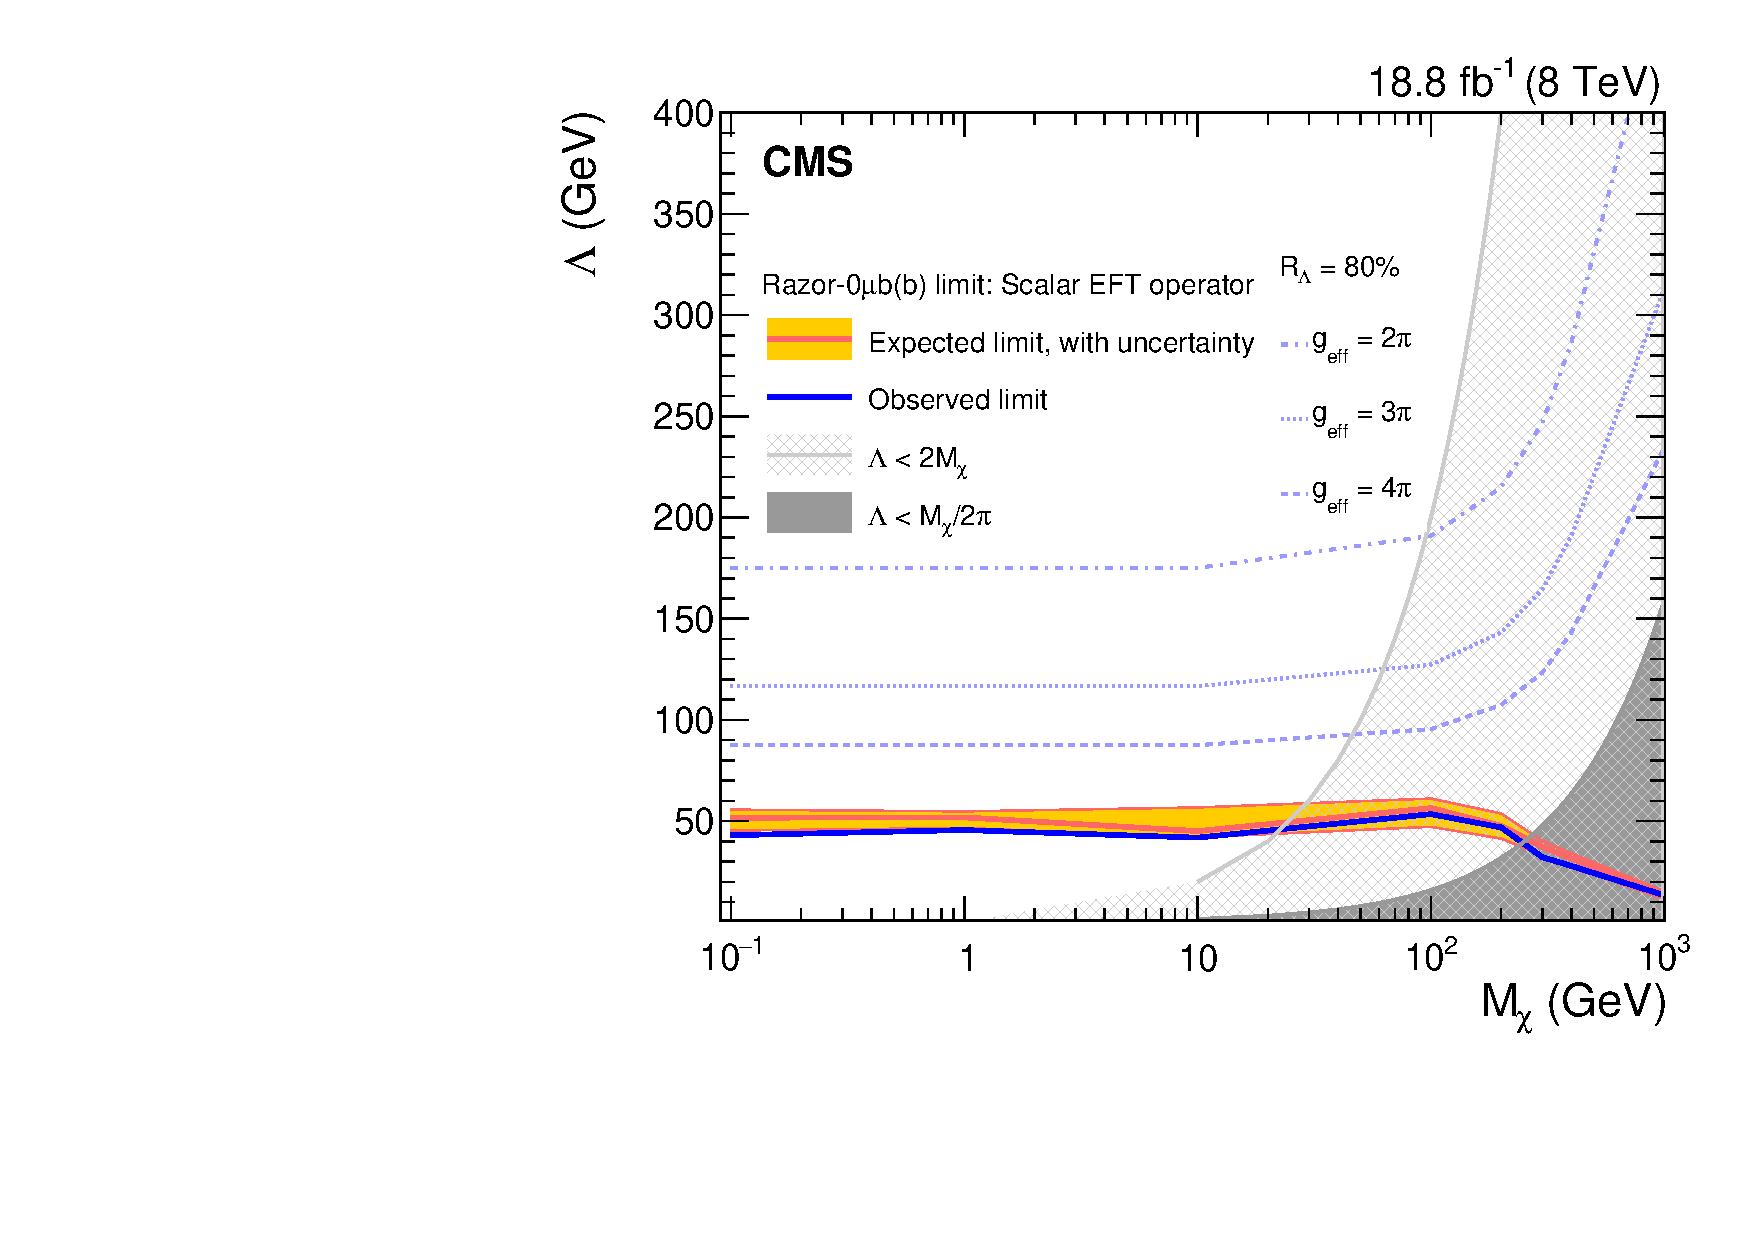
\includegraphics[width=0.5\textwidth]{DarkMatter8TeV/Limits/Final_MonoB_R80percent_vNov9_2015_CWR.pdf}  & 
  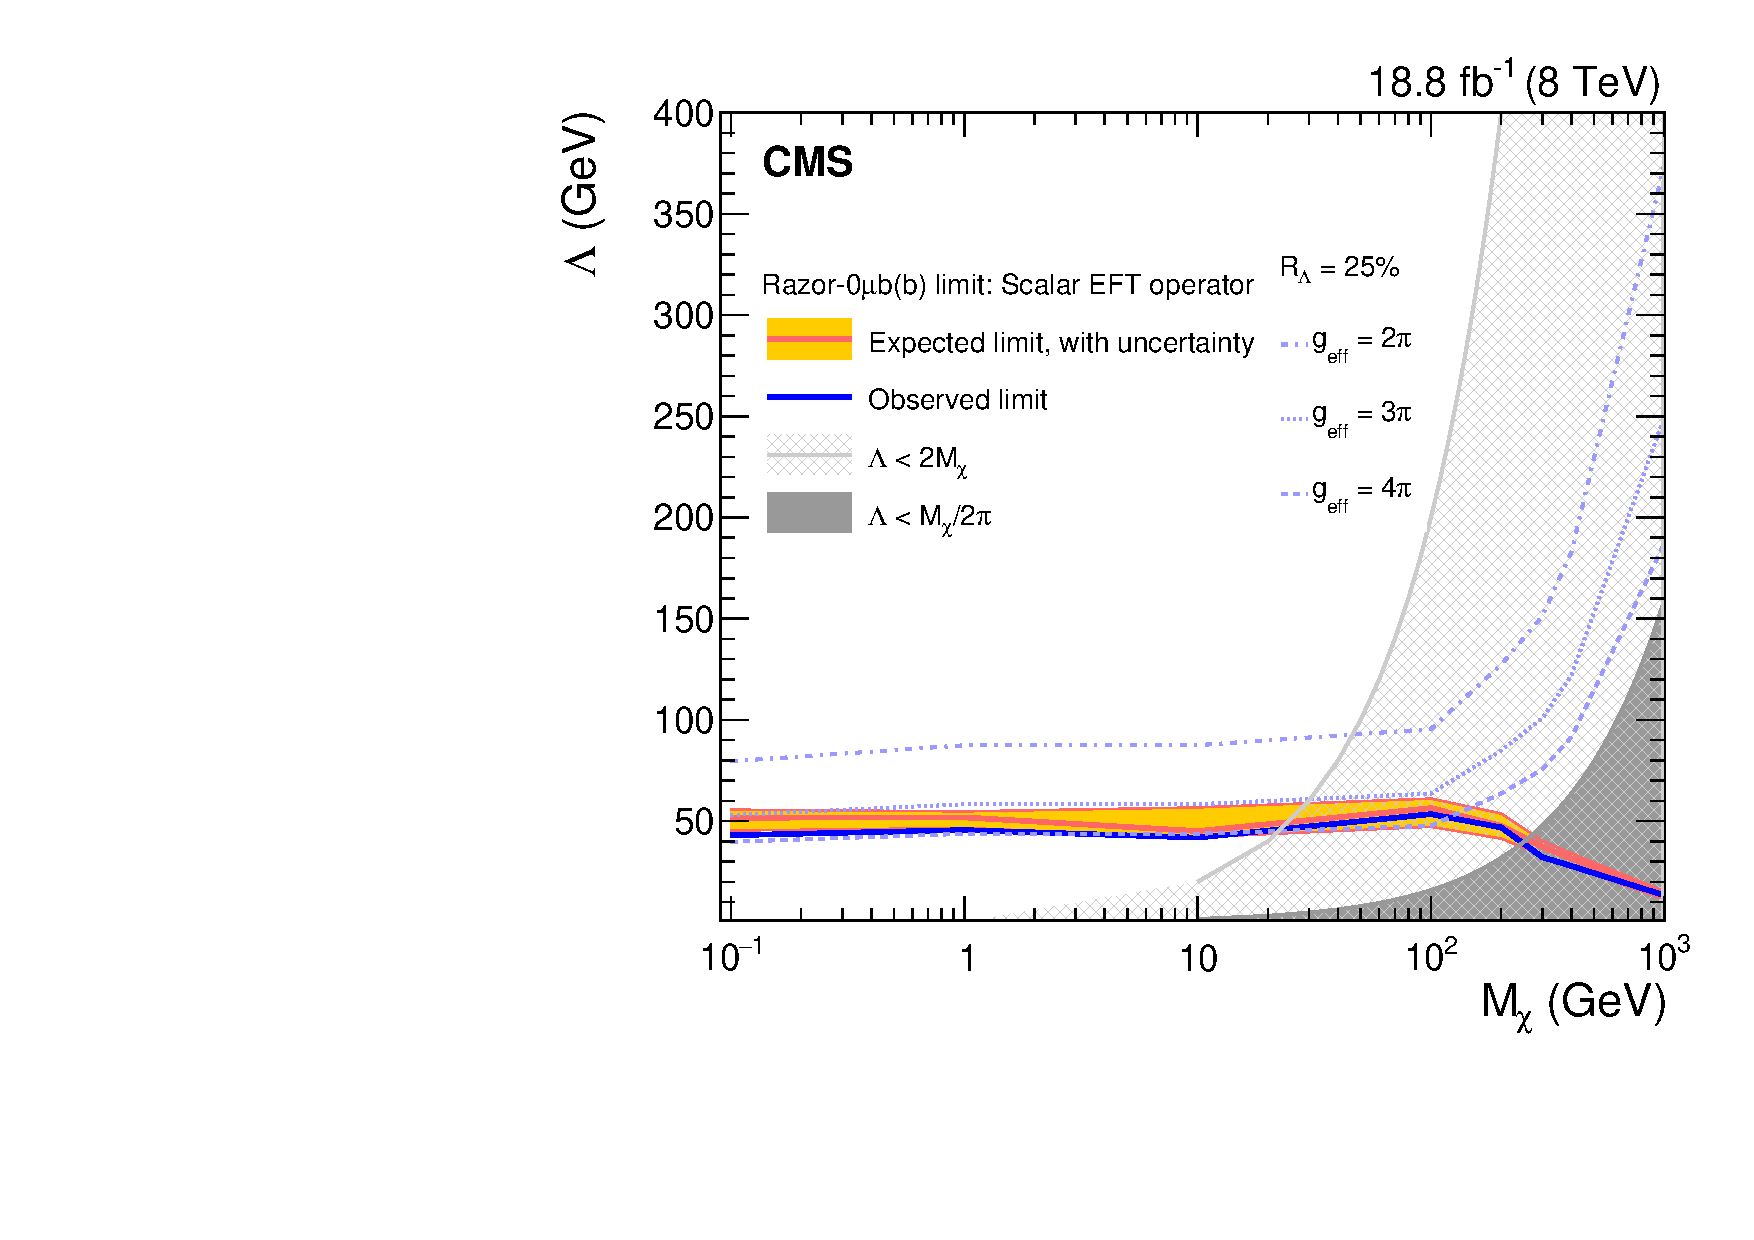
\includegraphics[width=0.5\textwidth]{DarkMatter8TeV/Limits/Final_MonoB_R25percent_vNov9_2015_CWR.pdf} \\
\end{tabular}
\caption{Lower limit at 90\% CL on the cutoff scale $\Lambda$ for the
  scalar operator $\hat{\mathcal{O}}_{S}$ as a function of the DM mass
  $\mathrm{M}_{\chi}$. The validity of the EFT is quantified by the
  $R_\Lambda = 80\%$ (left) and $R_\Lambda = 25\%$ (right) contours,
  corresponding to different values of the effective coupling
  $\math{g_{\rm eff}}$. \label{fig:LimitLambdab}}
\end{figure}

%The limit on the cutoff scale is translated into an upper limit on the
%spin-independent $\sigma_{N\chi}$~\cite{PhysRevD.88.063510} using the
%following expression:
%\begin{equation}
%  \sigma_{N\chi} \approx 2\times 10^{-38} \cm^{2} \left(\frac{30~\GeV}{\Lambda}\right)^{6} ,
%\end{equation}
%as shown in Fig.~\ref{fig:LimitbSI}.
%\begin{figure}[ht!]
 % \centering
 % 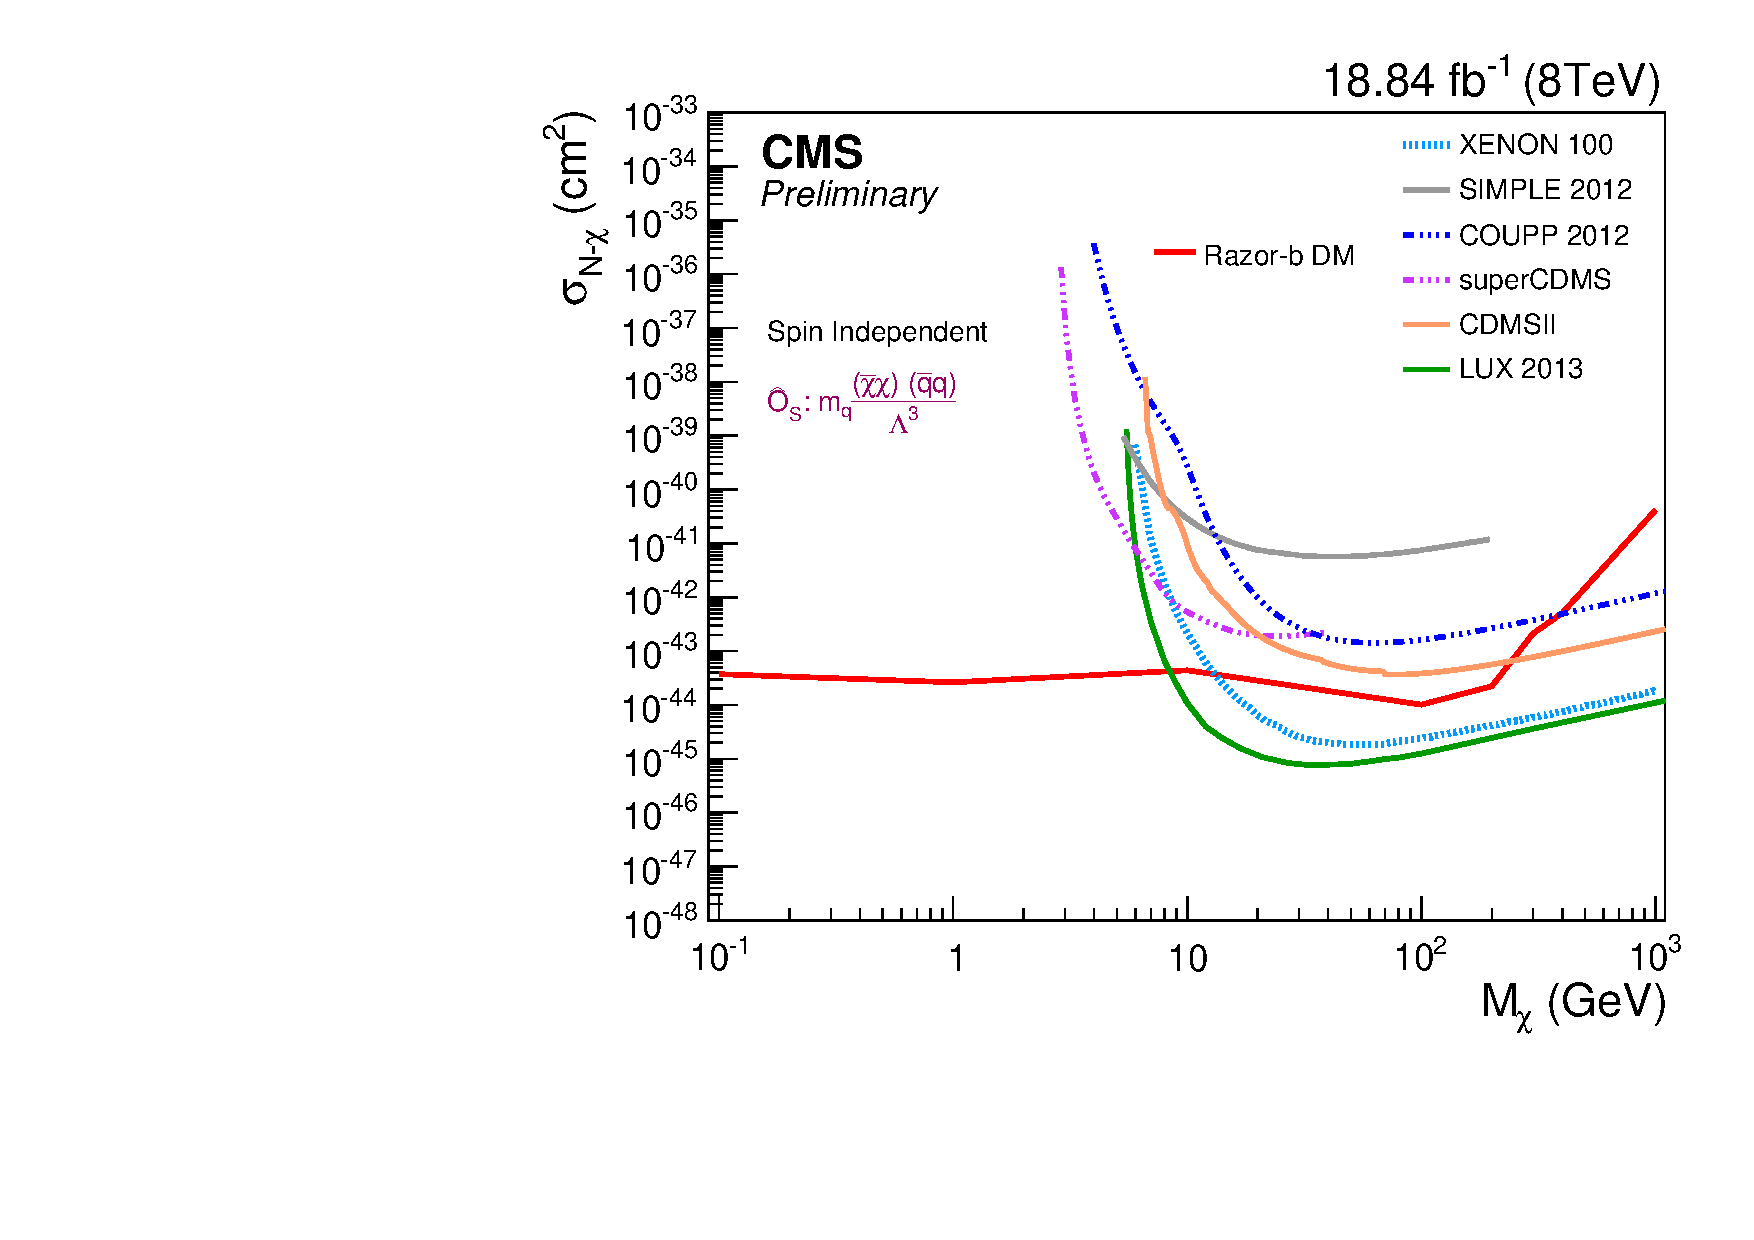
\includegraphics[width=0.5\textwidth]{Limits/SI_SigmaLimit_TOYS_razorB_March4.pdf}
 % \caption{Upper limit at 90\% CL on the spin-independent DM-nucleon
 %   scattering cross section $\sigma_{N\chi}$ as a function of the DM
 %   mass $\mathrm{M}_{\chi}$ for the scalar operator
 %   $\hat{\mathcal{O}}_{S}$ .\label{fig:LimitbSI}}
 % \end{figure}

\section{Summary}\label{sec:conclusions}

A search for dark matter has been performed studying proton-proton collisions collected
with the CMS detector at the LHC at a center-of-mass energy of
$8$~\TeV. The data correspond to an integrated luminosity of
$18.8$~\fbinv, collected with a dedicated high-rate trigger in 2012,
as parked data exercise, and processed during the LHC shutdown
in 2013.

Events with at least two jets are analyzed by studying the
distribution in the ($\mathrm{M_{\rm R}}$, $\mathrm{R}^2$) plane, in an
event topology complementary to that of monojet searches. Events with one or
two muons are used in conjunction with simulated samples, to predict
the expected background from standard model processes, mainly
$\cPZ$+jets and $\PW$+jets. The analysis is performed on events both
with and without b-tagged jets, originating from the hadronization of
a bottom quark, where in the latter case the dominant background comes from
$\ttbar$. The signal to background discrimination provided by the razor variables in conjunction with the exploration of events with small values of $\mathrm{M_{\rm R}}$ enabled by the exploitation of the parked data yield results that complement those previously published, thus enhancing the sensitivity to DM production in proton-proton collisions.

No significant excess is observed. The results are presented as
exclusion limits on dark matter production at 90\% CL for models based
on effective operators and for different assumptions on the
interaction between the DM particles and the colliding partons.

\section*{Acknowledgements}
We congratulate our colleagues in the CERN accelerator departments for
the excellent performance of the LHC and thank the technical and
administrative staffs at CERN and at other CMS institutes for their
contributions to the success of the CMS effort. In addition, we
gratefully acknowledge the computing centres and personnel of the
Worldwide LHC Computing Grid for delivering so effectively the
computing infrastructure essential to our analyses. Finally, we
acknowledge the enduring support for the construction and operation of
the LHC and the CMS detector provided by the following funding
agencies: the Austrian Federal Ministry of Science, Research and
Economy and the Austrian Science Fund; the Belgian Fonds de la
Recherche Scientifique, and Fonds voor Wetenschappelijk Onderzoek; the
Brazilian Funding Agencies (CNPq, CAPES, FAPERJ, and FAPESP); the
Bulgarian Ministry of Education and Science; CERN; the Chinese Academy
of Sciences, Ministry of Science and Technology, and National Natural
Science Foundation of China; the Colombian Funding Agency
(COLCIENCIAS); the Croatian Ministry of Science, Education and Sport,
and the Croatian Science Foundation; the Research Promotion
Foundation, Cyprus; the Ministry of Education and Research, Estonian
Research Council via IUT23-4 and IUT23-6 and European Regional
Development Fund, Estonia; the Academy of Finland, Finnish Ministry of
Education and Culture, and Helsinki Institute of Physics; the Institut
National de Physique Nucl\'eaire et de Physique des Particules~/~CNRS,
and Commissariat \`a l'\'Energie Atomique et aux \'Energies
Alternatives~/~CEA, France; the Bundesministerium f\"ur Bildung und
Forschung, Deutsche Forschungsgemeinschaft, and Helmholtz-Gemeinschaft
Deutscher Forschungszentren, Germany; the General Secretariat for
Research and Technology, Greece; the National Scientific Research
Foundation, and National Innovation Office, Hungary; the Department of
Atomic Energy and the Department of Science and Technology, India; the
Institute for Studies in Theoretical Physics and Mathematics, Iran;
the Science Foundation, Ireland; the Istituto Nazionale di Fisica
Nucleare, Italy; the Ministry of Science, ICT and Future Planning, and
National Research Foundation (NRF), Republic of Korea; the Lithuanian
Academy of Sciences; the Ministry of Education, and University of
Malaya (Malaysia); the Mexican Funding Agencies (CINVESTAV, CONACYT,
SEP, and UASLP-FAI); the Ministry of Business, Innovation and
Employment, New Zealand; the Pakistan Atomic Energy Commission; the
Ministry of Science and Higher Education and the National Science
Centre, Poland; the Funda\c{c}\~ao para a Ci\^encia e a Tecnologia,
Portugal; JINR, Dubna; the Ministry of Education and Science of the
Russian Federation, the Federal Agency of Atomic Energy of the Russian
Federation, Russian Academy of Sciences, and the Russian Foundation
for Basic Research; the Ministry of Education, Science and
Technological Development of Serbia; the Secretar\'{\i}a de Estado de
Investigaci\'on, Desarrollo e Innovaci\'on and Programa
Consolider-Ingenio 2010, Spain; the Swiss Funding Agencies (ETH Board,
ETH Zurich, PSI, SNF, UniZH, Canton Zurich, and SER); the Ministry of
Science and Technology, Taipei; the Thailand Center of Excellence in
Physics, the Institute for the Promotion of Teaching Science and
Technology of Thailand, Special Task Force for Activating Research and
the National Science and Technology Development Agency of Thailand;
the Scientific and Technical Research Council of Turkey, and Turkish
Atomic Energy Authority; the National Academy of Sciences of Ukraine,
and State Fund for Fundamental Researches, Ukraine; the Science and
Technology Facilities Council, UK; the US Department of Energy, and
the US National Science Foundation.

Individuals have received support from the Marie-Curie programme and the European Research Council and EPLANET (European Union); the Leventis Foundation; the A. P. Sloan Foundation; the Alexander von Humboldt Foundation; the Belgian Federal Science Policy Office; the Fonds pour la Formation \`a la Recherche dans l'Industrie et dans l'Agriculture (FRIA-Belgium); the Agentschap voor Innovatie door Wetenschap en Technologie (IWT-Belgium); the Ministry of Education, Youth and Sports (MEYS) of the Czech Republic; the Council of Science and Industrial Research, India; the HOMING PLUS programme of the Foundation for Polish Science, cofinanced from European Union, Regional Development Fund; the OPUS programme of the National Science Center (Poland); the Compagnia di San Paolo (Torino); MIUR project 20108T4XTM (Italy); the Thalis and Aristeia programmes cofinanced by EU-ESF and the Greek NSRF; the National Priorities Research Program by Qatar National Research Fund; the Rachadapisek Sompot Fund for Postdoctoral Fellowship, Chulalongkorn University (Thailand); the Chulalongkorn Academic into Its 2nd Century Project Advancement Project (Thailand); and the Welch Foundation, contract C-1845; and  the Weston Havens Foundation (USA).
\appendix 

\section*{Appendix}\label{sec:appendix}

%include{kin}

\section{Bin-by-bin background estimation and observed yield}

In this section, we provide the background estimate and the
observed yield for each bin of the ($\mathrm{M_{\rm R}}$, $\mathrm{R}^2$)
plane.
 
Tables~\ref{tab:LOOKUP_VL}-\ref{tab:LOOKUP_VH} show the expected and
observed yields in each $\mathrm{R}^2$ bin of each $\mathrm{M_{\rm R}}$
category for the 0$\mu$ sample.  Tables~\ref{tab:LOOKUP_B} and
\ref{tab:LOOKUP_BB} show the corresponding values for the 0$\mu$b and
the 0$\mu$bb samples, respectively.

\begin{table}[h!]
\begin{center}
  \caption{\label{tab:LOOKUP_VL} Background estimates and observed
    yield for each $\mathrm{R}^2$ bin in the VL $\mathrm{M_{\rm R}}$
    category.}
\begin{tabular}{|c|c|c|c|c|} 
  \hline
  $\mathrm{R^2}$ range & $0.5-0.55$ &  $0.55-0.6$ &  $0.6-0.65$ & $0.65-0.7$ \\
  \hline
  Observed & 2049 & 1607 & 1352 & 1147 \\
  \hline
  Estimated & 2350 $\pm$ 720  & 1810 $\pm$ 450 & 1530 $\pm$ 180 & 1240 $\pm$ 110\\
  \hline
  \hline
  $\mathrm{R^2}$ range & $0.7-0.75$ &  $0.75-0.8$ &  $0.8-0.85$ & $0.85-0.9$ \\
  \hline
  Observed & 1026 & 896 & 880 & 744 \\
  \hline
  Estimated & 1090 $\pm$ 140 & 1081 $\pm$ 76 & 876 $\pm$ 97 & 909 $\pm$ 63 \\
  \hline
  \hline
  $\mathrm{R^2}$ range  &  $0.9-0.95$  & $0.95-1.0$ & \multicolumn{2}{|c|}{$1.0-2.5$} \\
  \hline
  Observed  & 688 & 499 &  \multicolumn{2}{|c|}{735}  \\
  \hline
  Estimated & 674 $\pm$ 67 & 521 $\pm$ 43 &  \multicolumn{2}{|c|}{694  $\pm$ 62}  \\
  \hline
  \hline
\end{tabular}
\end{center}
\end{table}
\begin{table}[h!]
\begin{center}
  \caption{\label{tab:LOOKUP_L } Background estimates and observed
    yield for each $\mathrm{R}^2$ bin in the L $\mathrm{M_{\rm R}}$
    category.}
\begin{tabular}{|c|c|c|c|} 
  \hline
  $\mathrm{R^2}$ range & $0.5-0.575$ &  $0.575-0.65$ &  $0.65-0.75$  \\
  \hline
  Observed & 1088 & 765 & 682  \\
  \hline
  Estimated & 1220 $\pm$ 120 & 828 $\pm$ 65 & 810 $\pm$ 210 \\
  \hline
  \hline
  $\mathrm{R^2}$ range & $0.75-0.85$ &  $0.85-0.95$ &  $0.95-2.5$  \\
  \hline
  Observed & 565 & 395 & 290  \\
  \hline
  Estimated & 551 $\pm$ 59  & 454 $\pm$ 32 & 304 $\pm$ 43 \\
  \hline
 \hline
\end{tabular}
\end{center}
\end{table}
\newpage
\begin{table}[h!]
\begin{center}
  \caption{\label{tab:LOOKUP_H} Background estimates and observed
    yield for each $\mathrm{R}^2$ bin in the H $\mathrm{M_{\rm R}}$
    category.}
\begin{tabular}{|c|c|c|c|} 
  \hline
  $\mathrm{R^2}$ range & $0.5-0.575$ &  $0.575-0.65$ &  $0.65-0.75$  \\
  \hline
  Observed & 513 & 328 & 279 \\
  \hline
  Estimated & 560 $\pm$ 550 & 330 $\pm$ 360 & 275 $\pm$ 41 \\
  \hline
  \hline
  $\mathrm{R^2}$ range & $0.75-0.85$ &  $0.85-0.95$ &  $0.95-2.5$  \\
  \hline
  Observed & 203 & 151 & 85  \\
  \hline
  Estimated & 242 $\pm$ 18 & 171 $\pm$ 173 & 74 $\pm$ 17 \\
  \hline
  \hline
\end{tabular}
\end{center}
\end{table}
\begin{table}[h!]
\begin{center}
  \caption{\label{tab:LOOKUP_VH} Background estimates and observed
    yield for each $\mathrm{R}^2$ bin in the VH $\mathrm{M_{\rm R}}$
    category.}
\begin{tabular}{|c|c|c|c|c|} 
  \hline
  $\mathrm{R^2}$ range & $0.5-0.6$ &  $0.6-0.7$ &  $0.7-0.95$ & $0.95-2.5$ \\
  \hline
  Observed & 117 & 58 & 75 & 11 \\
  \hline
  Estimated & 100 $\pm$ 150 & 59 $\pm$ 36 & 75 $\pm$ 30 & 9 $\pm$ 7 \\
  \hline
\end{tabular}
\end{center}
\end{table}
%\clearpage
\begin{table}[h!]
\begin{center}
  \caption{\label{tab:LOOKUP_B}Background estimates and observed
    yield for each bin in the $0\mu$b signal region.}
\begin{tabular}{|c|c|c|c|c|} 
  \hline
  $\mathrm{R^2}$ range & $0.5-0.6$ &  $0.6-0.75$ &  $0.75-0.9$ & $0.9-2.5$ \\
  \hline
  Observed & 760 & 807 & 469 & 246 \\
  \hline
  Estimated & 850 $\pm$ 170 & 620 $\pm$ 120 & 470 $\pm$ 110 & 320 $\pm$ 160 \\
  \hline
\end{tabular}
\end{center}
\end{table}

\begin{table}[h!]
\begin{center}
  \caption{\label{tab:LOOKUP_BB}Background estimates and observed
    yield for each bin in the $0\mu$bb signal region.}
\begin{tabular}{|c|c|c|c|c|} 
  \hline
  $\mathrm{R^2}$ range & $0.5-0.6$ &  $0.6-0.75$ &  $0.75-0.9$ & $0.9-2.5$ \\
  \hline
  Observed & 122 & 80 & 31 & 14\\
  \hline
  Estimated & 135 $\pm$ 30 & 81 $\pm$ 18 & 36 $\pm$ 8 & 19 $\pm$ 9 \\
  \hline
\end{tabular}
\end{center}
\end{table}
%% **DO NOT REMOVE BIBLIOGRAPHY**

%%% DO NOT ADD \end{document}!
